\documentclass[letterpaper,12pt]{article}
\usepackage{tabularx} % extra features for tabular environment
\usepackage{amsmath}  % improve math presentation
\usepackage{graphicx} % takes care of graphic including machinery
\usepackage[margin=1in,letterpaper]{geometry} % decreases margins
\usepackage{xspace}
\usepackage{ANA-FTAG-2020-08-PAPER-defs}

\usepackage[style=numeric, sorting=none]{biblatex}
\addbibresource{ANA-FTAG-2020-08-PAPER.bib}
\addbibresource{bib/ATLAS.bib}
\addbibresource{bib/ATLAS-useful.bib}
\addbibresource{bib/PubNotes.bib}
\addbibresource{bib/ConfNotes.bib}
\addbibresource{bib/ATLAS-SUSY.bib}
\addbibresource{bib/*}
\usepackage[final]{hyperref} % adds hyper links inside the generated pdf file
\usepackage[T1]{fontenc}
\usepackage{setspace}
\usepackage{float}
\usepackage{makeidx}
\usepackage{titlesec}

\newcommand\bjetineq{\mathop{\mbox{$b$-$\mathit{jet}$}}}
\newcommand\bjetunder{\mathop{\footnotesize{\mbox{$b$-$\mathit{jet}$}}}\normalsize}
\newcommand\cjetineq{\mathop{\mbox{$c$-$\mathit{jet}$}}}
\newcommand\cjetunder{\mathop{\footnotesize{\mbox{$c$-$\mathit{jet}$}}}\normalsize}
\setcounter{secnumdepth}{4}

\titleformat{\paragraph}
{\normalfont\normalsize\bfseries}{\theparagraph}{1em}{}
\titlespacing*{\paragraph}
{0pt}{3.25ex plus 1ex minus .2ex}{1.5ex plus .2ex}
\restylefloat*{figure}
\hypersetup{
	colorlinks=true,       % false: boxed links; true: colored links
	linkcolor=blue,        % color of internal links
	citecolor=blue,        % color of links to bibliography
	filecolor=magenta,     % color of file links
	urlcolor=blue         
}

%++++++++++++++++++++++++++++++++++++++++
\linespread{1.17}
\makeindex
\begin{document}


\title{Search for di-Higgs in $bb\tau\tau$ final state using proton-proton collision at $\sqrt{s}$ = 13 \TeV\ data with the ATLAS detector}%Fake Factors Calculation and Implementation in H$\rightarrow$ bb$\tau^+\tau^-$ analysis with MC16a/MC16d in Release 21 with the ATLAS detector
\author{ Zhiyuan Li}
\date{\today}
\maketitle
\begin{figure}[htp]
\begin{minipage}[b]{.5\textwidth}
\centering

\includegraphics[width=1\textwidth]{logo.eps}
\end{minipage}\hfill
\begin{minipage}[b]{.45\textwidth}
\vspace{3em}
\centering

\includegraphics[width=1\textwidth]{ATLAS-Logo-Ref-RGB-H_1.jpg}
\end{minipage}
\end{figure}
\newpage


\tableofcontents{}
\printindex{}


\newpage
\section{Flavour tagging at ALTAS}
%test


\subsection{Flavour tagging}


The identification of jets containing $b$-hadrons ($b$-jets) 
against the large background of jets containing $c$-hadrons 
($c$-jets) or coming from the hadronization of light ($u$,$d$,$s$) 
quarks or gluons is of major importance in many areas of the 
physics programme of the ATLAS experiment at the LHC. It is 
crucial in the di-Higgs to $bb\tau\tau$ searches, as well as the recent 
observation of the Higgs boson decay into bottom quarks \cite{HIGG-2018-04} 
and of its production in association with a top-quark pair \cite{HIGG-2018-13}, 
and plays a important role in a large number of Standard Model (SM) 
precision measurements, studies of the Higgs boson properties, and 
searches for new phenomena\cite{SUSY-2014-08}, \cite{ATLAS-CONF-2018-043} \cite{Interpreting Higgs result}.

The ATLAS Collaboration uses various algorithms to identify 
$b$-jets \cite{PERF-2012-04}, referred to as b-tagging algorithms, 
when analysing data recorded during Run 2 of the LHC. These 
algorithms exploit the long lifetime, high mass and high decay 
multiplicity of b-hadrons as well as the properties of the b-quark 
fragmentation. Given a lifetime of the order of 1.5 ps 
($<c\tau>$ $\approx$ 450 $\mu m$), measurable b-hadrons have a 
significant mean flight length,$<l>$=$\beta\gamma c\tau$, in the 
detector before decaying, generally leading to at least one vertex 
displaced from the hard-scatter collision point. The strategy 
developed by the ATLAS Collaboration is based on a two-stage approach. 
Firstly, low-level algorithms reconstruct the characteristic features of 
the $b$-jets via two complementary approaches, one that uses the 
individual properties of charged-particle tracks, later referred 
to as tracks, associated with a hadronic jet, and a second which 
combines the tracks to explicitly reconstruct displaced vertices. 
These algorithms, first introduced during Run 1 \cite{PERF-2012-04}, 
have been improved and retuned for Run 2. Secondly, in order to 
maximise the b-tagging performance, the results of the low-level 
b-tagging algorithms are combined in high-level algorithms 
consisting of multivariate classifiers. The performance of a 
b-tagging algorithm is characterised by the probability of 
tagging a $b$-jet ($b$-jet tagging efficiency, $\epsilon_b$) and 
the probability of mistakenly identifying a $c$-jet or a light-flavour 
jet as a $b$-jet, labelled $\epsilon_c$($\epsilon_l$). 

In this chapter, the performance of the algorithms is quantified 
in terms of $c$-jet and light-flavour jet rejections, defined as 
1/$\epsilon_c$ and 1/$\epsilon_l$, respectively. The imperfect 
description of the detector response and physics modelling effects 
in Monte Carlo (MC) simulations necessitates the measurement of the 
performance of the b-tagging algorithms with collision data 
\cite{PERF-2012-04 ttbar,b-jet identification semi ttbar}. 
In this chapter, the measurement of the $b$-jet tagging efficiency 
of the high-level b-tagging algorithms used in proton–proton (pp) 
collision data recorded during Run 2 of the LHC at $\sqrt{s}$ = 13 TeV 
is presented. The corresponding measurements for $c$-jets and light-flavour 
jets, used in the measurement of the $b$-jet tagging efficiency to correct 
the simulation such that the overall tagging efficiency of $c$-jets and 
light-flavour jets match that of the data, are described elsewhere 
\cite{ATLAS-CONF-2018-006}, \cite{cjet}. The production of $t\bar{t}$ 
pairs at the LHC provides an abundant source of $b$-jets by virtue 
of the high cross-section and the $t \rightarrow Wb$ branching ratio 
being close to 100\%. A very pure sample of $t\bar{t}$ events is 
selected by requiring that both $W$ bosons decay leptonically, 
referred to as di-leptonic $t\bar{t}$ decays in the following. 
Similarly a source of $c$-jets can be obtained by requiring that 
one $W$ boson decay leptonically and the other decay hadronically, 
referred to as semi-leptonic $t\bar{t}$ decay in the following. 


% The identification of the jets originating from the hadronization of heavy-flavour quarks is made possible by the distinctive properties of the heavy hadrons produced in the process. For instance, the large life time of $b$-quarks allows them to travel a measurable distance from the primary interaction point before to decay, giving rise to displaced tracks which can form secondary vertices. The ATLAS Collaboration developed several algorithms to identify (tag) the jets from $b$-quark hadronization based on the properties detailed above. 

The most performant algorithms presently in use in physics 
analyses at ATLAS are based on multivariate (MV2) combinations 
of the available information or a deep feed-forward neural 
network(DL1)\cite{tagging}\cite{ATL-PHYS-PUB-2017-013}, as shown in 
Figure \ref{fig:MV2_DL1}. Depending on the low-level algorithm, 
the DL1 tagger can be further separated into two taggers: DL1 and DL1r,
 where the DL1 tagger uses traditional track-based impact parameter 
 taggers IP2D and IP3D and DL1r tagger uses a Recurrent Neural Network tagger 
 (RNNIP)\cite{ATL-PHYS-PUB-2017-013}. The DL1r tagger is now the 
 default b-tagging algorithm used for flavour tagging in ATLAS.
%Their high mass also leads to decay products with a larger transverse momentum relative to the jet axis with respect to the ones typically found in jets from light partons. Finally, heavy hadrons have a sizable branching ratio for semileptonic decays, hence the presence of soft leptons in the produced jets provides another tool for heavy jet identification. %The general strategy is to start with simple algorithms that exploits a particular property of b jets and progressively add more information to build moresophisticated algorithms. %The output of these algorithms consists in a discriminant value for each jet. Operating points are then defined as thresholds on the discriminant, designed to provide a determined efficiency for identifying b jets.
% Low-level $b$-taggingalgorithms fall into two broad categories. A first approach, implemented in the IP2D and IP3D algorithms \cite{ATL-PHYS-PUB-2017-013}, or RNNIP \cite{ATL-PHYS-PUB-2017-003} is inclusive and based on exploiting the large impact parameters of the tracks originating from the $b$-hadron decay. The second approach explicitly reconstructs displaced vertices. To maximise the $b$-tagging performance, low-level algorithm results are combined using multivariate classifiers. To this end, two high-level tagging algorithms have been developed. The first one,MV2\cite{ATL-PHYS-PUB-2017-013}, is based on a boosted decisiontree (BDT) discriminant, while the second one,DL1, is based on a deep feed-forward neural network(NN). These two algorithms are presented in fig .
\begin{figure}
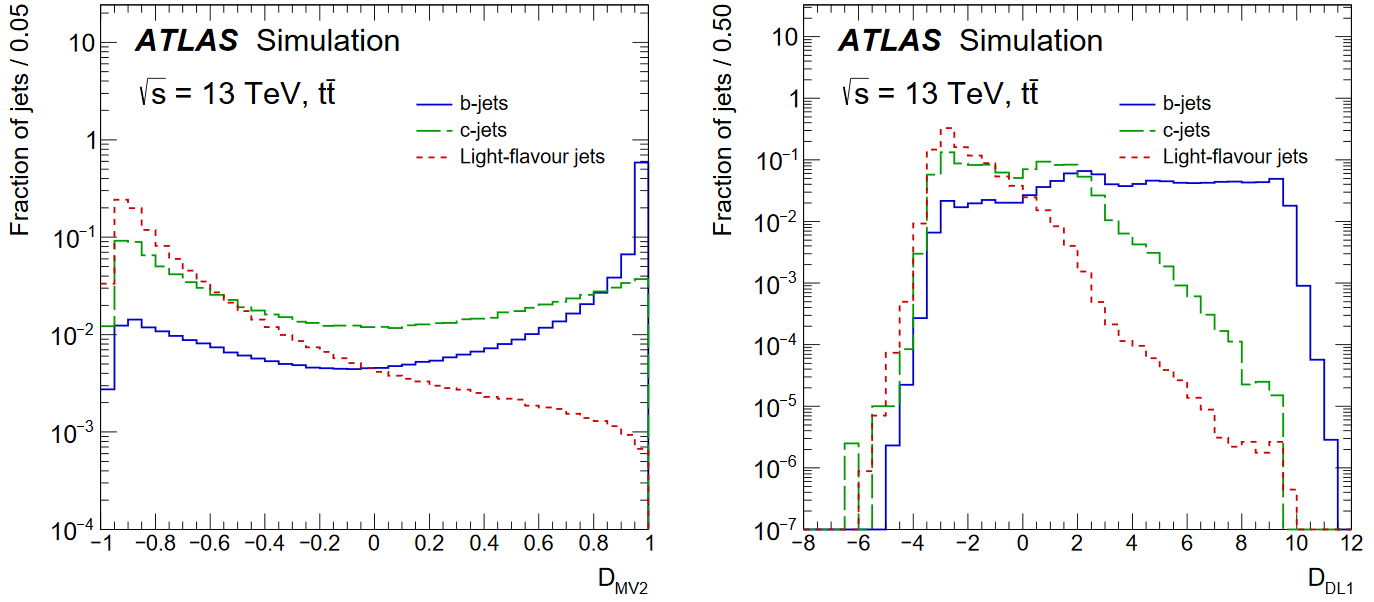
\includegraphics[width=1\textwidth]{MV2_DL1.png}
\caption{Performance of MV2c10 and DL1 tagger\cite{FTAG-2018-01}.}\label{fig:MV2_DL1}
\end{figure}

\subsection{Calibration methods}
Monte Carlo (MC) simulations are not able to model very well the 
performance of the $b$-tagging algorithms in data. For this reason 
calibration is required, i.e. correcting MC to match the data 
in terms of $b$-tagging efficiency, charm-jet mis-tagging and 
light-jet mis-tagging rates\cite{FTAG-2018-01}. The calibration is done 
for all supported working points, which are cuts in the b-tagging 
algorithm output identifying the tagging efficiencies, and jet 
collections(TODO: refer back to the object definition chapter). 
In general, the efficiency is calculated with data and simulations, 
and scale factors are then calculated to match the efficiency extracted 
from simulations to the data. More details of the calibrations of 
different flavour are given in the following subsections.


For the \bjet\ calibration, the performance of the $b$ tagging 
algorithms is evaluated in the simulation and the efficiency 
with which these algorithms identify jets containing $b$-hadrons 
is measured in collision data. The measurement uses a likelihood-based 
method in a di-leptonic (both $W$ bosons from the top decay decay 
into leptons) $t\bar{t}$ sample of highly enriched in $t\bar{t}$ 
events. Events with 2 jets and 2 opposite signs leptons are selected 
from di-leptonic $t\bar{t}$ samples. The data $b$-jet efficiency is 
then extracted from a combined likelihood fit, and subsequently 
compared with that predicted by the simulation. Scale factors are 
then calculated to match the performance of the algorithms to the data\cite{FTAG-2018-01}.

For the light jet mis-tagging calibration, two methods are 
used to measure the mistagging rate from the data: the negative 
tag method, which uses a high statistics data sample enriched 
in light-jets with the application of a modified algorithm which 
reverses some of the criteria used in the nominal identification 
algorithm, and the adjusted Monte Carlo (adjusted-MC) method, which 
adjusts the characteristic track observables in the simulation 
to match the data, and then compares the adjusted simulation to the 
"standard" simulation. The scale factors are then calculated using 
the these two methods. The scale factors of the two different methods 
are in good agreement within the systematics uncertainties\cite{ATLAS-CONF-2018-006}. 
%The aim of this calibration is to calibrate $b$-jets that have been mis-tagged as light-jets of b-tagging algorithm. As the $b$-tagging algorithm is very efficient in rejecting light-jets, the light-jet fraction is enriched via "flipped" taggers, which negates the sign of track IP parameters before $b$-tagging\cite{ATLAS-CONF-2018-006}. The calibrations of the standard and the 'flipped' tagger are assumed to be equal. The calibration is extracted using the leading $p_T$ jet of Z+jets events using a 2D fit. TODO: cite the light-jet tagging Int note
%light-jet fractions in the $b$-like region are too low,  The Z + jets events are then selected, the secondary vertex mass is fitted to obtain flavour fractions and perform a likelihood fit to extract light-jet mistag rate.

The charm-jet mis-tagging calibration utilises semi-leptonic $t\bar{t}$ 
events. The events kinematics are shown by the diagram in 
Figure \ref{fig:feynman}, where the $t\bar{t}$ pair decays to a 
pair of $b$ and $\bar{t}$ quark, circled in red. One of the $W$ boson, 
circled in blue, decays hadronically to quarks, and the other $W$ boson, 
decays leptonically to either electron or muon and the corresponding neutrinos, 
circled in purple and green. The lepton in the final state is used for 
triggering, and a combined likelihood fit is used to extract the $c$ mis-tagging 
efficiency (more details in Section \ref{charm mistagging}). 

\begin{figure}[H]
\centering
\begin{minipage}[b]{.45\textwidth}
\centering
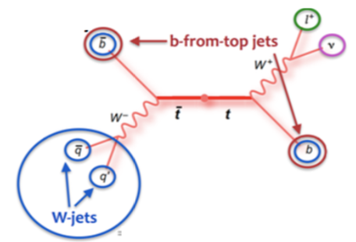
\includegraphics[width=1\textwidth]{feynman.png}
\end{minipage}
\caption{Feynman diagram of the semi-leptonic $t\bar{t}$ events.}
\label{fig:feynman}
\end{figure}
\section{Charm mis-tagging calibration}
\label{charm mistagging}
\subsection{Introduction}
%As Shown in Fig \ref{fig:feynman}, the calibration uses the semi-leptonic $t\bar{t}$ events, which one $W$ boson from top decays leptonically to a charged lepton and neutrino and one $W$ decays hadronically and dominantly to a charm and a strange quark, among other pairs.
As determined by the CKM matrix\cite{CKM1}\cite{CKM2}, the $W$ boson decay to light-quark pair or 
light quark $c$ quark pair dominantly, and very rarely decay to pairs containing $b$-quarks. 
More specifically, the branching ratio of a $W$ boson decays to a pair of light quarks or a light quark 
and a $c$ quark is 33.7\%, and of pairs containing a b quark is only 0.058\%\cite{PDG}. 
Therefore, $b$-tagged jets from the $W$ decay are most likely to be mis-tagging of $c$-jets or 
light-jets. Given the ratio between the DL1 light-jet rejection and the corresponding charm-jet rejection 
ranges from 10 to 40 (see ref\cite{ATL-PHYS-PUB-2017-013}), the 
$c$-jet in $c$-jet-light-jet pairs is the most likely source for the 
$b$-tagged jet. A kinematic likelihood technique, referred to as 
KLFitter\cite{ERDMANN201418}, is used to assign jets to the proper $t\bar{t}$ decay product 
without using any $b$-tagging information (more details in Section \ref{KLFitter}). 
The charm-jet efficiency is then extracted by a combinatorial likelihood fit applying to the pair 
of jets from $W$ decays, where the main floating parameter is the $c$-jet efficiency\cite{cjet}. 

It is worth mentioning that my qualification task to become an ATLAS author is to 
calibrate the rate of a charm jet being mis-identified as a $b$-jet, which is a part 
of the calibration of the $b$-tagging algorithm. The calibration uses the full Run2 data 
of 139 fb$^{-1}$ integrated luminosity collected at $\sqrt{s}$ = 13 TeV by the ATLAS detector. 
In the task, 4 rounds of calibration has been conducted, each round with different jet collection 
and b-tagging algorithm. To be concise only the result of the last round is presented in this chapter. 
During the task the calibration range has been extended down to 20 GeV (which was 25 GeV) and a new 
selection category has been developed to increase the stats of the scale factors in the 
high $p_T$ ($p_T$ greater than 70 GeV) region.

\subsection{Data and Monte Carlo samples}
%%%%%%%%%%%%%%%%%%%%%%%%%%%%%%%%%%%%%%%%%%%%%%%

\label{sec:samples}
%%%%%%%%%%%%%%%%%%%%%%%%%%%%%%%%%%%%%%%%%%%%%%%
The data analysed in this study correspond to 139~fb$^{-1}$~\cite{DAPR-2010-01,DAPR-2011-01,DAPR-2013-01,LUCID2}, 
of \(pp\) collision data collected by the ATLAS detector between 2015 and 2018
with a centre-of-mass energy of 13~\TeV\ and a 25\,ns proton bunch
crossing interval. 
The data sample was collected using a set of single-muon~\cite{Aad:2020uyd} 
and single-electron triggers~\cite{TRIG-2018-05}. The single-muon triggers 
had \pt\ thresholds in the range of 20--26~\GeV\ for 
isolated muons and 50~\GeV\ for muons without any isolation requirement. 
The single-electron triggers employed a range of \pt\ thresholds in the range 24--300~\GeV\ 
and a combination of quality and isolation requirements depending on the 
data-taking period and the \pt\ threshold.
%The uncertainty in the combined 2015--2018
%integrated luminosity is 1.7\%~\cite{ATLAS-CONF-2019-021}, obtained
%using the LUCID-2 detector~\cite{LUCID2} for the primary luminosity
%measurements. 
All detector subsystems were required to be operational
during data taking and to fulfil data quality requirements.  

% The $t\bar{t}$ samples and the single top-quark in the Wt 
% and s-channel samples are generated with the {\tt Powheg-Box} v2 \cite{powheg} 
% generator. Electroweak t-channel single top-quark events are generated 
% using the {\tt Powheg-Box} v1 generator. The parton shower, fragmentation, 
% and the underlying event are simulated using {\tt Pythia} 6.428\cite{pythia} 
% with the CTEQ6L1 PDF sets and the corresponding Perugia 2012 tune (P2012)\cite{perugia}. 
% The top-quark mass is set to 172.5 GeV. The {\tt EvtGen} v1.2.0 program \cite{evtgen} 
% is used to model the properties of the bottom and charm hadron decays. 
% The $t\bar{t}$ production cross-section is calculated at NNLO+NNLL 
% (next-to-next-to-leading-logarithm)\cite{NNLO}. For single-top processes, 
% the generator NLO cross-sections are used. Events containing $W$ or $Z$ 
% bosons with associated jets are simulated using {\tt Sherpa} 2.2.1\cite{sherpa}. 
% All $W$/$Z$+jets events are normalised to the predicted cross-sections using 
% NNLO calculations. All samples are passed through the full GEANT4\cite{GEANT4} 
% simulation of the ATLAS detector and are reconstructed with the same software as used for data.



Dedicated Monte Carlo  simulated samples (MC)  are used to model SM
processes and to estimate the expected signal yields.  All samples were 
produced using the ATLAS simulation infrastructure~\cite{SOFT-2010-01}
and $\GEANT4$~\cite{Agostinelli:2002hh}. A subset of samples use a faster 
simulation based on a parameterisation of the calorimeter response and 
$\GEANT4$ for the other detector systems~\cite{SOFT-2010-01}. %\cite{ATL-PHYS-PUB-2010-013}.
The simulated events are reconstructed with the same algorithms as
used for data, and contain a realistic modelling of pile-up
interactions. The pile-up profiles in the simulation match those of each dataset
between 2015 and 2018, and are obtained by overlaying minimum-bias events,
simulated using the soft QCD processes of
{\PYTHIA}~8~\cite{Sjostrand:2014zea} using the NNPDF2.3LO set of
PDFs~\cite{Ball:2012cx} and a set of tuned
parameters called the A3 tune~\cite{ATL-PHYS-PUB-2016-017}.

The events that are used in this study originate mostly due to \
ttbar\ production. This process is modelled using the
\powhegbox~v2~\cite{Frixione:2007nw,Nason:2004rx,Frixione:2007vw,Alioli:2010xd}
generator at NLO with the \nnpdfnlo % ~\cite{Ball:2014uwa}
parton distribution function (PDF) set
and the \hdamp\ parameter\footnote{The
  \hdamp\ parameter is a resummation damping factor and one of the
  parameters that controls the matching of \powheg matrix elements to
  the parton shower and thus effectively regulates the
  high-\pt\ radiation against which the \ttbar\ system recoils.} set
to 1.5~\mtop~\cite{ATL-PHYS-PUB-2016-020}.  The events were interfaced
to {\PYTHIA}~8.230 to model the parton shower,
hadronisation, and underlying event, with parameters set according
to the A14 tune and using the \nnpdftwo set of PDFs.
The decays of bottom and charm hadrons were performed by \evtgen~v1.6.0~\cite{EvtGen}.


%%% single top
In addition to \ttbar\ production, there are some minor backgrounds
that contribute to the final event sample that is used for the calibration.
These backgrounds consist mostly of single-top and diboson production, 
the production of \ttbar\ in association with a vector boson
and the production of a vector boson in association with jets.
The details
of the modeling of these samples are given in the following.

Single-top $s$-channel production is modelled using the \powhegbox~v2 % \cite{Alioli:2009je,Nason:2004rx,Frixione:2007vw,Alioli:2010xd}
generator at NLO in QCD in the five-flavour scheme with the \nnpdfnlo~\cite{Ball:2014uwa} parton distribution function~(PDF) set.
%The events are interfaced with \pythia.230 % ~\cite{Sjostrand:2014zea} 
%using the A14 tune % ~\cite{ATL-PHYS-PUB-2014-021}
%and the \nnpdftwo PDF set.
%
The associated production of top quarks with $W$ bosons ($tW$) is
modelled using the
\powhegbox~v2~\cite{Re:2010bp,Nason:2004rx,Frixione:2007vw,Alioli:2010xd}
generator at NLO in QCD using the five-flavour scheme and the
\nnpdfnlo set of PDFs~\cite{Ball:2014uwa}.
The diagram removal scheme~\cite{Frixione:2008yi} is used to
remove interference and overlap with \ttbar\ production. 
The events for both single-top $s$-channel and $tW$ production 
are interfaced to \pythia.230%~\cite{Sjostrand:2014zea} 
using the A14 tune%~\cite{ATL-PHYS-PUB-2014-021} 
and the \nnpdftwo set of PDFs. %~\cite{Ball:2012cx}.

The production of $Z+$jets and $W$+jets is simulated with the
\sherpa~v2.2.1~\cite{Bothmann:2019yzt}
generator using next-to-leading order (NLO) matrix elements (ME) for up to two partons, and leading order (LO) matrix elements
for up to four partons calculated with the Comix~\cite{Gleisberg:2008fv}
and \openloops~\cite{Buccioni:2019sur,Cascioli:2011va,Denner:2016kdg} libraries. They
are matched with the \sherpa parton shower~\cite{Schumann:2007mg} using the MEPS@NLO
prescription~\cite{Hoeche:2011fd,Hoeche:2012yf,Catani:2001cc,Hoeche:2009rj}
using the set of tuned parameters developed by the \sherpa authors.
The \nnpdfnnlo set of PDFs~\cite{Ball:2014uwa} is used and the samples
are normalised to a next-to-next-to-leading order (NNLO)
prediction~\cite{Anastasiou:2003ds}.

Samples of diboson final states ($VV$) are simulated with the
\sherpa~v2.2.1 or v2.2.2~\cite{Bothmann:2019yzt} generator depending on the process,
%~\footnote{This is an admixture of 2.2.1 and above versions, so the version should be kept generic to avoid confusions. As an alternative, the sentence can be modified indicating that samples are simulated with the \sherpa~v2.2.1 or v2.2.2 depending on the process.} 
including off-shell effects and Higgs-boson contributions, where appropriate.
Fully leptonic final states and semileptonic final states, where one boson
decays leptonically and the other hadronically, are generated using
matrix elements at NLO accuracy in QCD for up to one additional parton
and at LO accuracy for up to three additional parton
emissions. Samples for the loop-induced processes $gg \to VV$ are
generated using LO-accurate matrix elements for up to one
additional parton emission for both cases of fully leptonic and
semileptonic final states. The matrix element calculations are matched
and merged with the \sherpa parton shower based on Catani-Seymour
dipole factorisation~\cite{Gleisberg:2008fv,Schumann:2007mg} using the MEPS@NLO
prescription~\cite{Hoeche:2011fd,Hoeche:2012yf,Catani:2001cc,Hoeche:2009rj}.
The virtual QCD correction are provided by the
\openloops library~\cite{Buccioni:2019sur,Cascioli:2011va,Denner:2016kdg}. The
\nnpdfnnlo set of PDFs is used, %~\cite{Ball:2014uwa}, 
along with the dedicated set of tuned parton-shower parameters developed by the
\sherpa authors.

The production of \ttbar\ in assosiation with a vector boson 
is modelled using the
\mgamc~v2.3.3~\cite{Alwall:2014hca} generator at NLO with the
\nnpdfnlo~\cite{Ball:2014uwa} parton distribution function~(PDF).
The events are interfaced to \pythia.210~\cite{Sjostrand:2014zea}~
using the A14 tune~\cite{ATL-PHYS-PUB-2014-021} and the
\nnpdftwo~\cite{Ball:2014uwa} PDF set. The decays of bottom and charm
hadrons are simulated using the \evtgen\ v1.2.0 program~\cite{Lange:2001uf}.



\subsection{Kinematic Likelihood Fitter}
\label{KLFitter}
% Top quarks decay to a $W$ boson and a bottom quark in nearly 100\% of all 
% cases. Consequently, the final state of a top-quark pair is characterised by 
% the decay products of the two $W$ bosons. 
% %If one of the $W$ bosons decays into a charged lepton and a neutrino while the other one decays into a pair of quarks, the decay mode is referred to as the single-lepton, or semi-leptonic decay mode. 
% The fraction of top-quark pairs decaying either in the 
% single-electron or single-muon decay mode 
% is about 30\%. The corresponding event signature is defined 
% by exactly one electron or muon, four jets out of which 
% two contain a $b$-hadron, and a large amount of missing transverse momentum 
% due to the un-detected neutrino. The Kinematic Likelihood Fitter\cite{ERDMANN201418}, 
% is a reconstruction technique developed to reconstruct $t\bar{t}$ decays, 
% which exploits the above decay topology of the top quark in the 
% semi-leptonic channel in order to properly associate jets to the 
% quarks in the final state of the decay process. In the semi-leptonic 
% decay of the $t\bar{t}$ system, the resulting tree level situation 
% contains two $b$-quarks from the top quark decays, and two light or 
% charm quarks from the $W$ boson decay (Figure \ref{fig:feynman}). 
% A likelihood is used to properly assign these four jets to the true 
% decay quarks. The leading order scenario is assumed, giving rise to four jets 
% in the final $t\bar{t}$ decay topology, two of which are $b$-jets. Three 
% of the jets in the decay are associated to the hadronic top decay, 
% whereas a final fourth jet along with the charged lepton and 
% neutrino build the leptonic top\cite{cjet}.
The four-vectors of the four highest \pt\ jets, the lepton and the
event \MET\ are used as inputs to a likelihood-based \ttbar\ event
reconstruction algorithm, which is described in more detail in
Ref.~\cite{ERDMANN201418}. This algorithm uses a likelihood function
to assign the four jets to the \ttbar\ decay topology. In particular,
the algorithm assigns one jet to be \bjet\ from the leptonically
decaying top-quark ($t\to Wb \to \ell \nu b$) one other to the \bjet\
from the hadronically decaying top-quark ($t\to Wb \to qq^\prime b$,
where $qq^\prime$ are the quarks in which the $W$ boson decays) and
the remaining two jets to the jets that come from the hadronic $W$
boson decay. The jet assignment does not use any \btagging\ information.
The following notation will be used: the jets that are
assigned as the decay products of the $W$ boson are referred to as
$W$-jets and the remaining two jets are referred to as top-jets.

\subsubsection{Maximising likelihood}
\label{maximise likelihood}
Taking only four jets in the event limits the total number of possible 
jet orderings (permutations) in the event. In the semi-leptonic channel, 
four jets can be permuted a total number of times equal to 4! = 24. 
However, the two jets (from light or $c$-quarks) resulting from the 
hadronic $W$ decay are kinematically indistinguishable. This reduces 
the possible number of permutations to 12. Furthermore, no $b$-tagging 
information is used in the kinematic likelihood to limit the possible number of permutations.
For every combination of jet ordering the likelihood is maximised over 
its free parameters, the energy of the four jets, the lepton energy and 
the three components of the momentum of the neutrino, and provides a 
value based on how closely the kinematic information from the reconstructed 
objects for a specific jet ordering resembles the expected kinematic behaviour 
of the decay of a Standard Model semi-leptonic $t\bar{t}$ event. The likelihood 
therefore distinguishes the possible permutations on an event-by-event basis. 
The best permutation, given by the largest log-likelihood value, is adopted 
as the jet ordering for the event\cite{cjet}. To improve the purity of the 
selected events further, an additional requirement of log-likelihood > -48 is 
placed on the output of the likelihood value for the chosen event permutation. 
An example of the distribution of log-likelihood of the best permutations 
is shown in Figure \ref{fig:llr}. 
In this figure, the data events are compared against the simulation.
The majority of the events come from \ttbar\ production. There is only
a very small fraction of events, which is denoted as ``non \ttbar''
on the figure, which comes from other processes like $W$ or $Z$ production
in association with jets or single-top production. The simulated \ttbar\
events are split according to the origin of $W$-jets. The notation
``\ttbar, ll'' denotes that both $W$-jets are light flavour jets.
Similarly, ``\ttbar, cl'' (``\ttbar, bl'') 
indicates that one of the $W$-jets is a \cjet\ (\bjet)
whereas the other is a light flavour jet. $W$-jets with origin
other than what is discussed above fall into the 
category denoted by ``\ttbar, other''. This category includes
events in which at least one of the $W$-jets comes from a
hadronically decaying $\tau$-lepton. 



\begin{figure}%[htb]
	\centering
	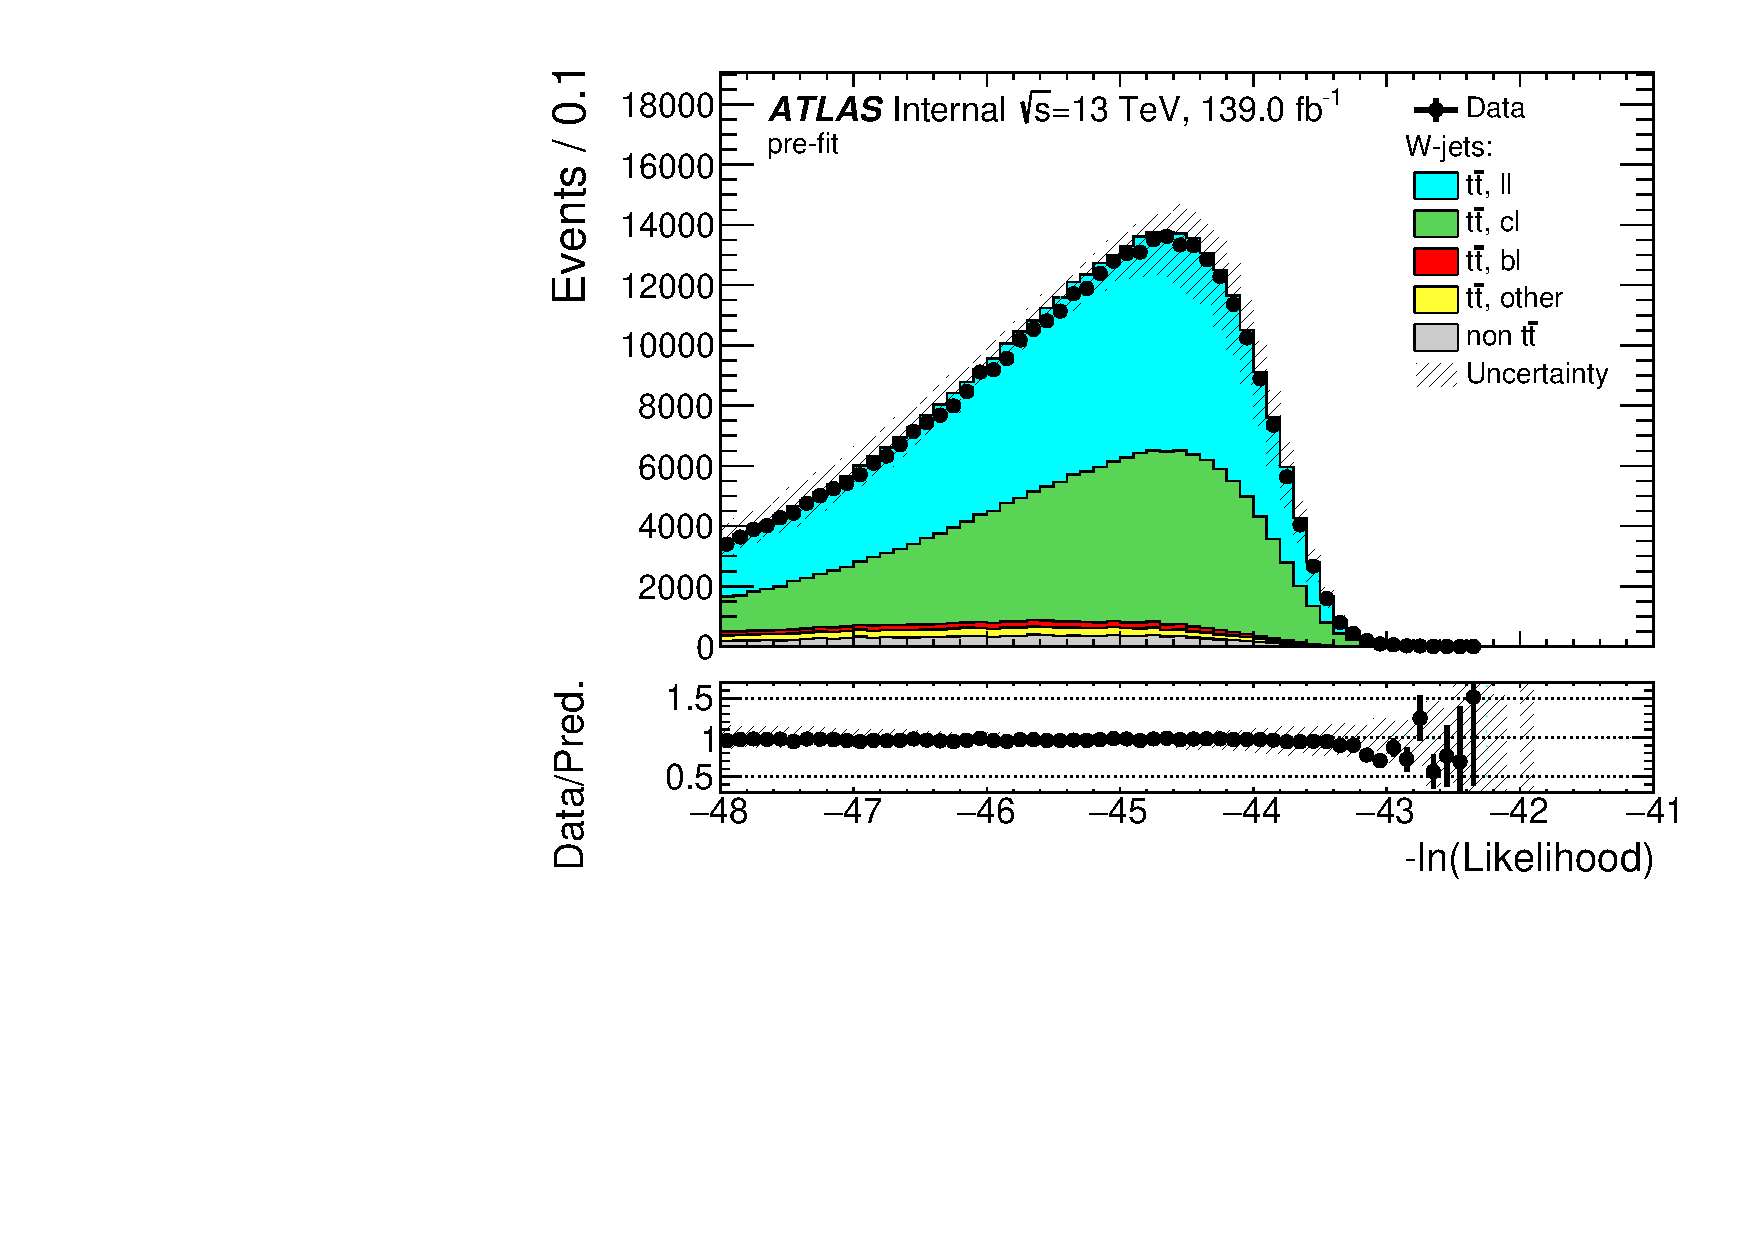
\includegraphics[width=0.45\textwidth]{prefit/DataMC_h_LLR_all_3bunc.pdf}
	\caption{Distribution of  the negative logarithm of the likelihood that
	is used to reconstruct the \ttbar\ decay.}
	\label{fig:llr}
\end{figure}



% \subsubsection{KLFitter Jet selection}
% In the standard selection, only events with exactly 4 jets are selected. 
% Therefore, there is no room for wrong choice of choosing 4 jets out of 4 jets, 
% which will then be the input for the KLFitter tool (More details can be found 
% in section \ref{standard selection}). However, this becomes a problem when the 
% 4 jets requirement is lifted. In the selection for reducing errors in high-$p_{T}$ 
% bins of scale factors (referred to as high-$p_{T}$ selection from now on, more 
% details can be found in section \ref{high_pt_selection}), events with at least 5 
% jets can also pass the selection. Therefore how to choose the 4 jets out of the 5 
% jets and possibly more jets is now a problem. Without using any b-tagging information, 
% the best solution in this case would be to simply select the 4 jets with the highest $p_T$. %In the June 2019 Charm calibration and calibrations before that, the 'kBtagPriorityFourJets' selection mode was used, which will select the 4 jets highest $p_T$ while prioritising the $b$-jets. This was not a problem until the high-$p_{T}$ selection was introduced. With this particular mode an anomaly was observed in the $b$-jet purity in the reconstructed $W$ boson decay jets, when comparing the combination of the high-$p_{T}$ selection and the standard selection to the standard selection, as shown in Figure \ref{fig:highpt}(a)(b). 
% To check the impact of including more then 4 jets in the events, the $b$-jet purity 
% was checked, which is defined as:
% \begin{equation}
% \bjetineq purity= \frac{N_{true\ \bjetunder}}{N_{all}},
% \end{equation}
% where $N_{true \bjetunder}$ stands for the number of events 
% with a true $b$-jet from the $W$ decay, 
% and $N_{all}$ stands for the number of all events.
% As shown in Figure \ref{fig:highpt}(a)(b), less $b$-jets are 
% presented in the high-$p_{T}$ selection. This difference can be reduced 
% after applying $b$-tagging of jets passing DL1r at 60\% working point 
% as shown in Figure \ref{fig:highpt}(c)(d). The $b$-jet purity after $b$-tagging 
% is defined as:
% \begin{equation}
% \bjetineq\ purity\ after\ tagging= \frac{N_{true\ tagged\ \bjetunder}}{N_{tagged}},
% \end{equation}
% where $N_{true\ tagged\ \bjetunder}$ stands for the number of events with a true tagged $b$-jet from the $W$ decay, and $N_{tagged}$ stands for the number of events with a tagged $b$-jet from the $W$ decay.
% \begin{figure}[H]
% \centering

% \begin{minipage}[b]{.45\textwidth}
% \centering
% 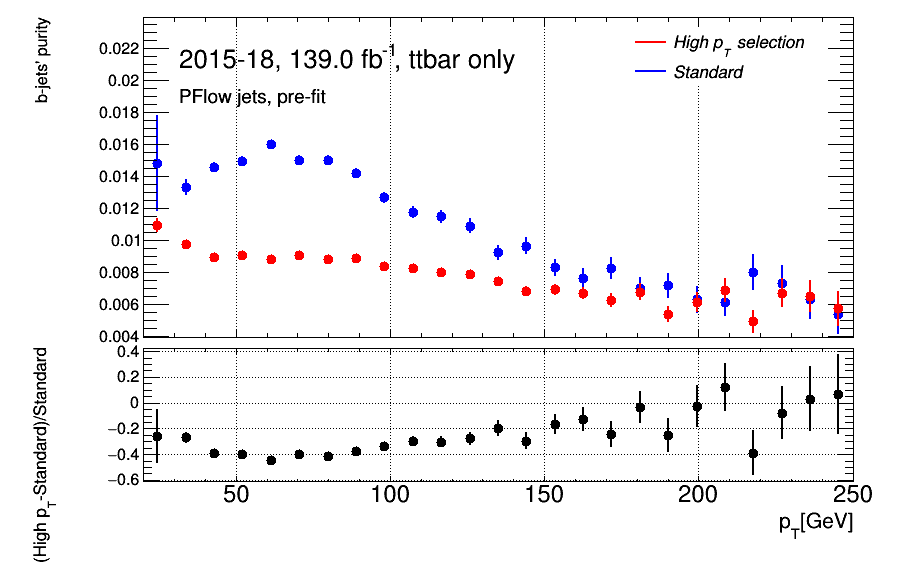
\includegraphics[width=1\textwidth]{b_purity/_stats_bjets_purityp_Tjet0GeV.eps}
% \footnotesize (a) Comparing the leading jet $b$-jet purity distribution 
% between the standard selection and the high $p_T$ selection.\label{fig:b_after_leading}
% \end{minipage}\hfill
% \begin{minipage}[b]{.45\textwidth}
% \centering
% 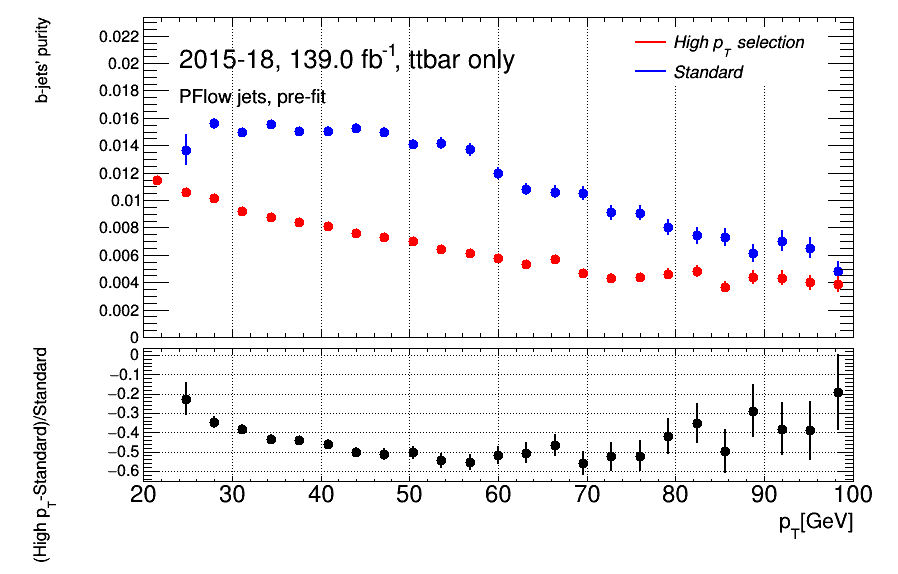
\includegraphics[width=1\textwidth]{b_purity/_stats_bjets_purityp_Tjet1GeV.eps}
% \footnotesize (b) Comparing the sub-leading jet $b$-jet 
% purity distribution between the standard selection and the high $p_T$ selection.\label{fig:b_after_subleading}
% \end{minipage}\hfill
% \begin{minipage}[b]{.45\textwidth}
% \centering
% 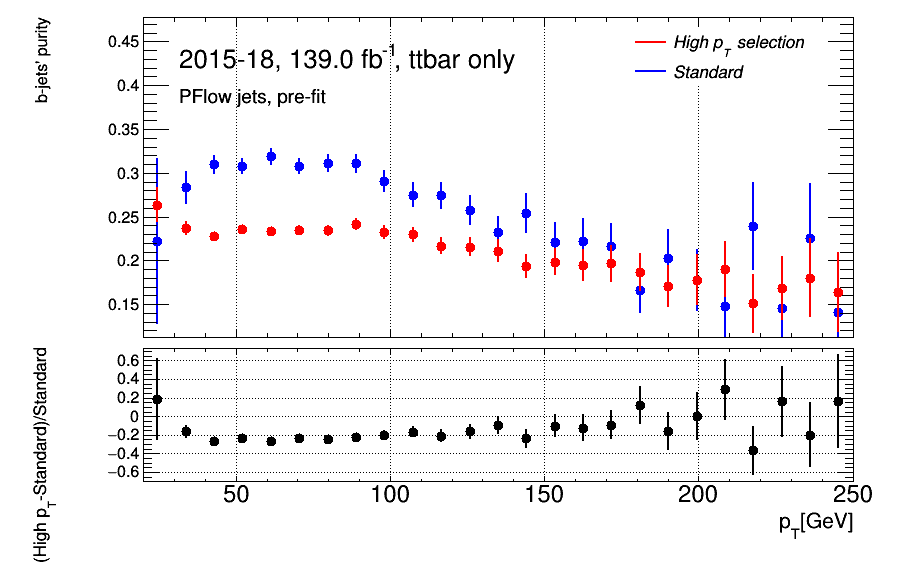
\includegraphics[width=1\textwidth]{b_purity/tagged_stats_bjets_purityp_Tjet0GeV.eps}
% \label{b_tagged_leading}
% \footnotesize (c) Comparing the leading jet $b$-jet purity distribution 
% between the standard selection and the high $p_T$ selection after 
% applying $b$-tagging with DL1r tagger at 60\% working point.
% \end{minipage}\hfill
% \begin{minipage}[b]{.45\textwidth}
% \centering
% 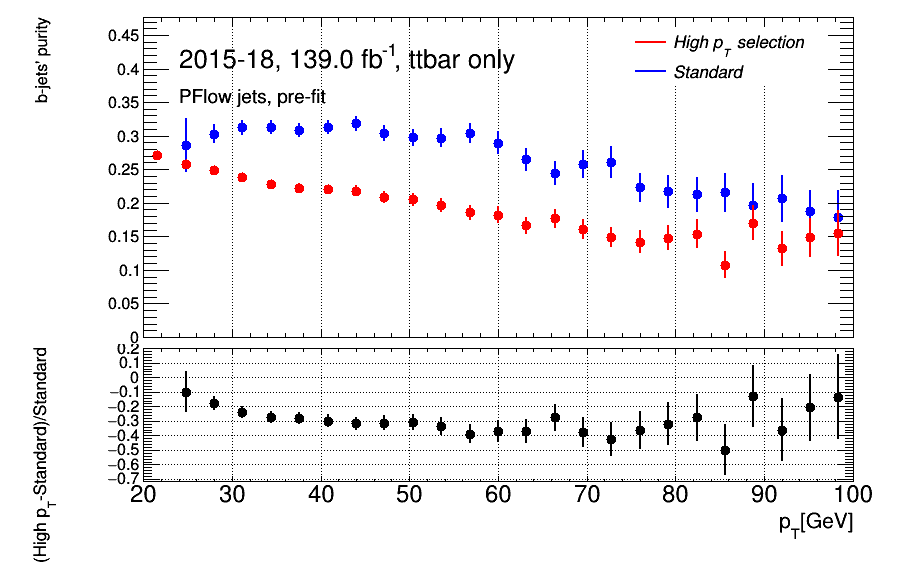
\includegraphics[width=1\textwidth]{b_purity/tagged_stats_bjets_purityp_Tjet1GeV.eps}
% \label{b_tagged_subleading}
% \footnotesize (d) Comparing the sub-leading jet $b$-jet purity 
% distribution between the standard selection and the high $p_T$ 
% selection after applying $b$-tagging with DL1r tagger at 60\% working point.
% \end{minipage}
% \caption{Comparison of the $b$-jet purity in leading (the left column) 
% and sub-leading (the right column) jet $p_{T}$ distribution.}
% \label{fig:highpt}
% \end{figure}

\subsection{Event selection}
\label{Event selection}
 % The analysis uses the full available integrated luminosity collected with the ATLAS detector from the all years. This corresponds to a collected luminosity of 139 fb$^{-1}$. The event selection aims to select a sample enriched in $t\bar{t}$ events. The lowest un-prescaled single electron and single-muon triggers are used.


\subsubsection{Standard selection}
\label{standard selection}
Events are required to contain exactly one trigger-matched 
lepton with $p_{T}$ above 27 GeV and exactly four jets with 
$p_{T}$ above 25 GeV. Leptons are required to have $p_{T}$ 
above 27 GeV in order to avoid the turn-on curve for the 
single lepton triggers. Events which contain an additional 
lepton with $p_T$ above 27 GeV are rejected. 
In addition, events are required 
to have a minimum of 20 GeV missing transverse momentum, which is 
assumed to be the result of the neutrino from the leptonically 
decaying $W$ boson. 
The events are also required to have $\MET > 20$~\GeV\ and the transverse
mass $m_T$ between the lepton and the \MET, is
constrained as follows:
\[ m_T = \sqrt{2 p_T^\ell \MET (1-\cos\Delta\phi)} > 40~\GeV,\]
where $\Delta\phi = \phi(\MET)-\phi(\ell)$ is the azimuthal difference between
the lepton and \MET.
For each event, the kinematic likelihood fitter 
is applied which determines the jet assignment to the various top 
decay products assumed from the $t\bar{t}$ decay products. 
A requirement of the log of KLFitter output > -48 is placed 
on the chosen event permutation. 
Due to the requirement on jet $p_T$ and binning strategy, the calibration 
result can be applied to jets with $p_{T}$ between 25 to 200 GeV. 
The inclusive yields of the standard selection and the low \pt\ selection 
(defintion in Section \ref{fig:lowpT_selection})of the data/MC are 
given in Table \ref{tab:yields_standard}, an example of 
the \pt\ distributions before any tagging or fitting and 
after the standard selection is shown in Figure \ref{fig:kinematic_distributions_standard}. 
More plots can be found in Appendix, Figure \ref{fig:standard_selection}.
The meaning of each legend in the plots are described in Section \ref{maximise likelihood}. 
The yellow band in the lower pad shows the overall systematics uncertainties combining the 
experimental uncertainties and the \ttbar\ modelling uncertainties, as described in 
Section \ref{systematic uncertainties.} The data/MC ratio shows good agreement 
within the systematic uncertainties. 

\begin{table}[!b]
	\centering
	\small
	\setlength\tabcolsep{5pt} 
	\begin{tabular}{|l | ll | ll |}
	\hline
	& \multicolumn{2}{c|}{Particle flow jets} & \multicolumn{2}{c|}{Track jets} \\
	\hline
	Data          &    287105.0                  &        &   218351.0                  &     \\  
	Ttbar         &    292203.7 $\pm$       202.8 &        &   223769.3 $\pm$       177.6 &   \\
	Other         &     10945.7 $\pm$       123.1 &        &     7280.1 $\pm$       103.1 &   \\
	Data/MC       &     0.947   $\pm$       0.002 &        &    0.945   $\pm$        0.002  &           \\
	\hline
	% \multicolumn{5}{|c|}{Comparison of \ttbar\ with systematic samples}\\
	% \hline
	% TtbarAF2       & 294528.0 $\pm$  225.3   &  0.795\%   & 225611.0 $\pm$  197.3 &  0.823\%  \\
	% DATA/MC(AF2)   & 0.940    $\pm$  0.002   &            &    0.938 $\pm$  0.002 &           \\              
	% TtbarRadHi     & 286717.9 $\pm$  197.8   & -1.877\%   & 219779.4 $\pm$  174.4 &  -1.783\%  \\     
	% DATA/MC(RADHI) &  0.965   $\pm$  0.002   &            &    0.962 $\pm$  0.002 &             \\       
	% TtbarPH        & 222493.6 $\pm$  173.7   & -23.857\%  & 167600.2 $\pm$  152.1 &  -25.101\% \\ 
	% DATA/MC(PH)    & 1.230    $\pm$  0.003   &            &    1.249 $\pm$  0.003 &            \\                
	% \hline
	\end{tabular}
	\vspace{0.2cm}
	\caption{Prefit comparison of the  number of events in data and in 
	simulation considering particle flow jets and track jets for 
	events with exactly 4 jets, combining with the low \pt\ selection.}
	\label{tab:yields_standard}
	\end{table}


 \begin{figure}%[htb]
	\centering
	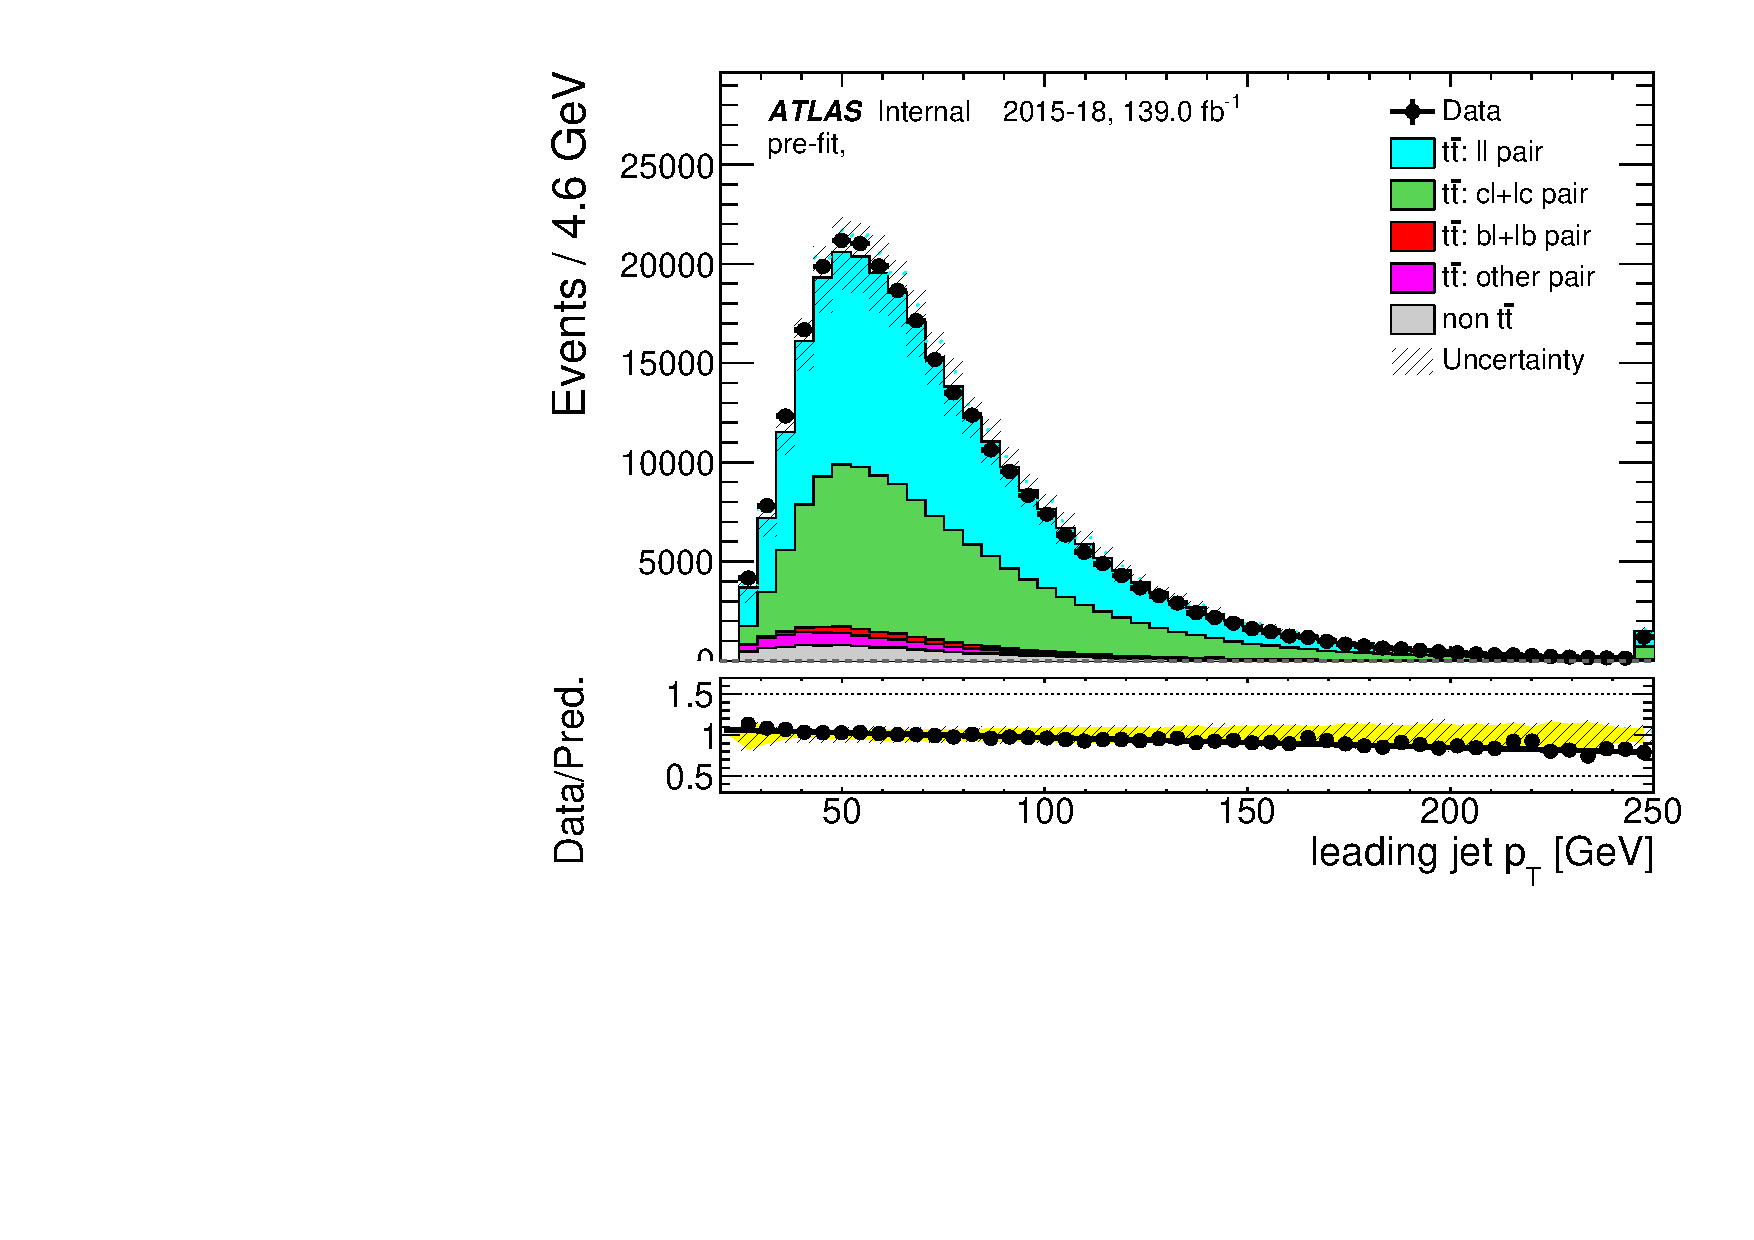
\includegraphics[width=0.45\textwidth]{figs_support/plots_withoutHighpT/DataMC_h_J0_pt.pdf}
	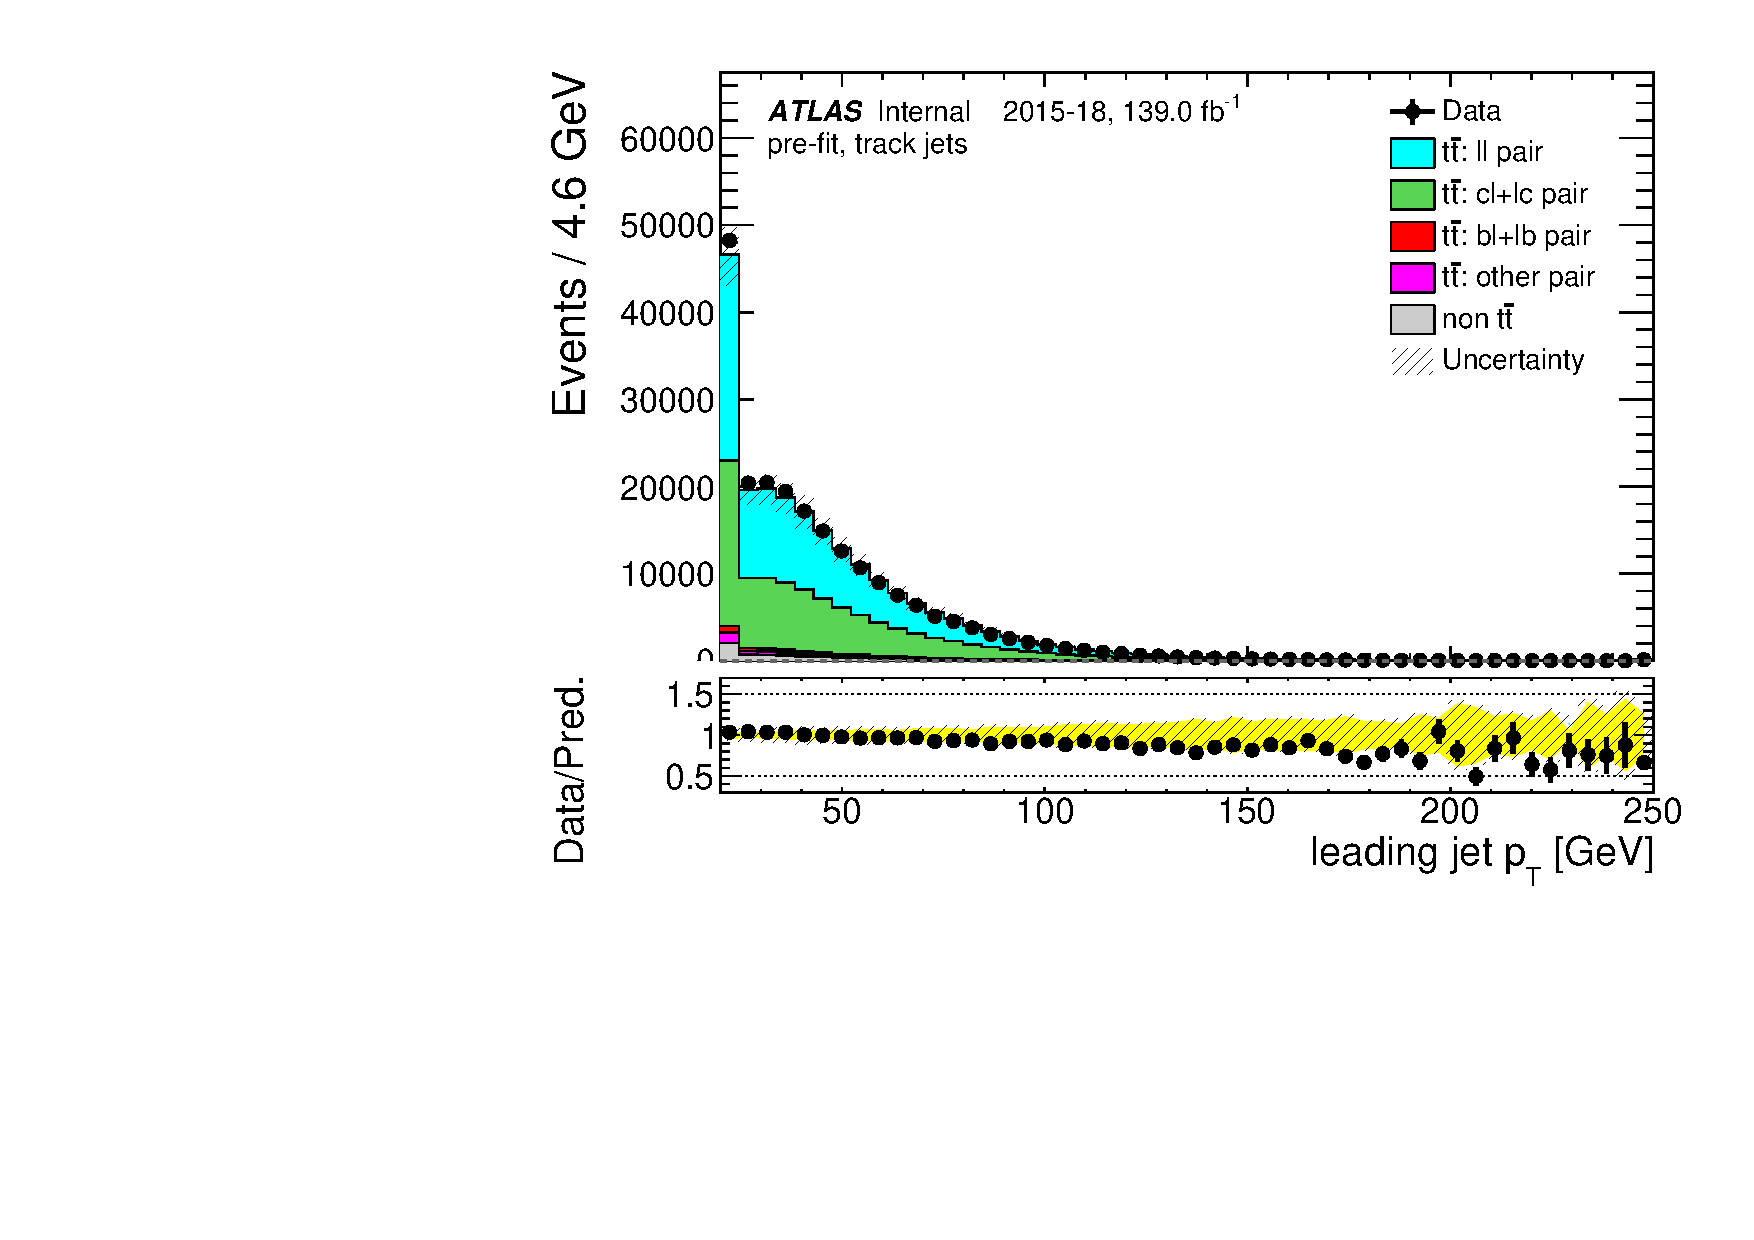
\includegraphics[width=0.45\textwidth]{figs_support/plots_withoutHighpT/DataMC_h_J0_pttrackjet.pdf}\\
	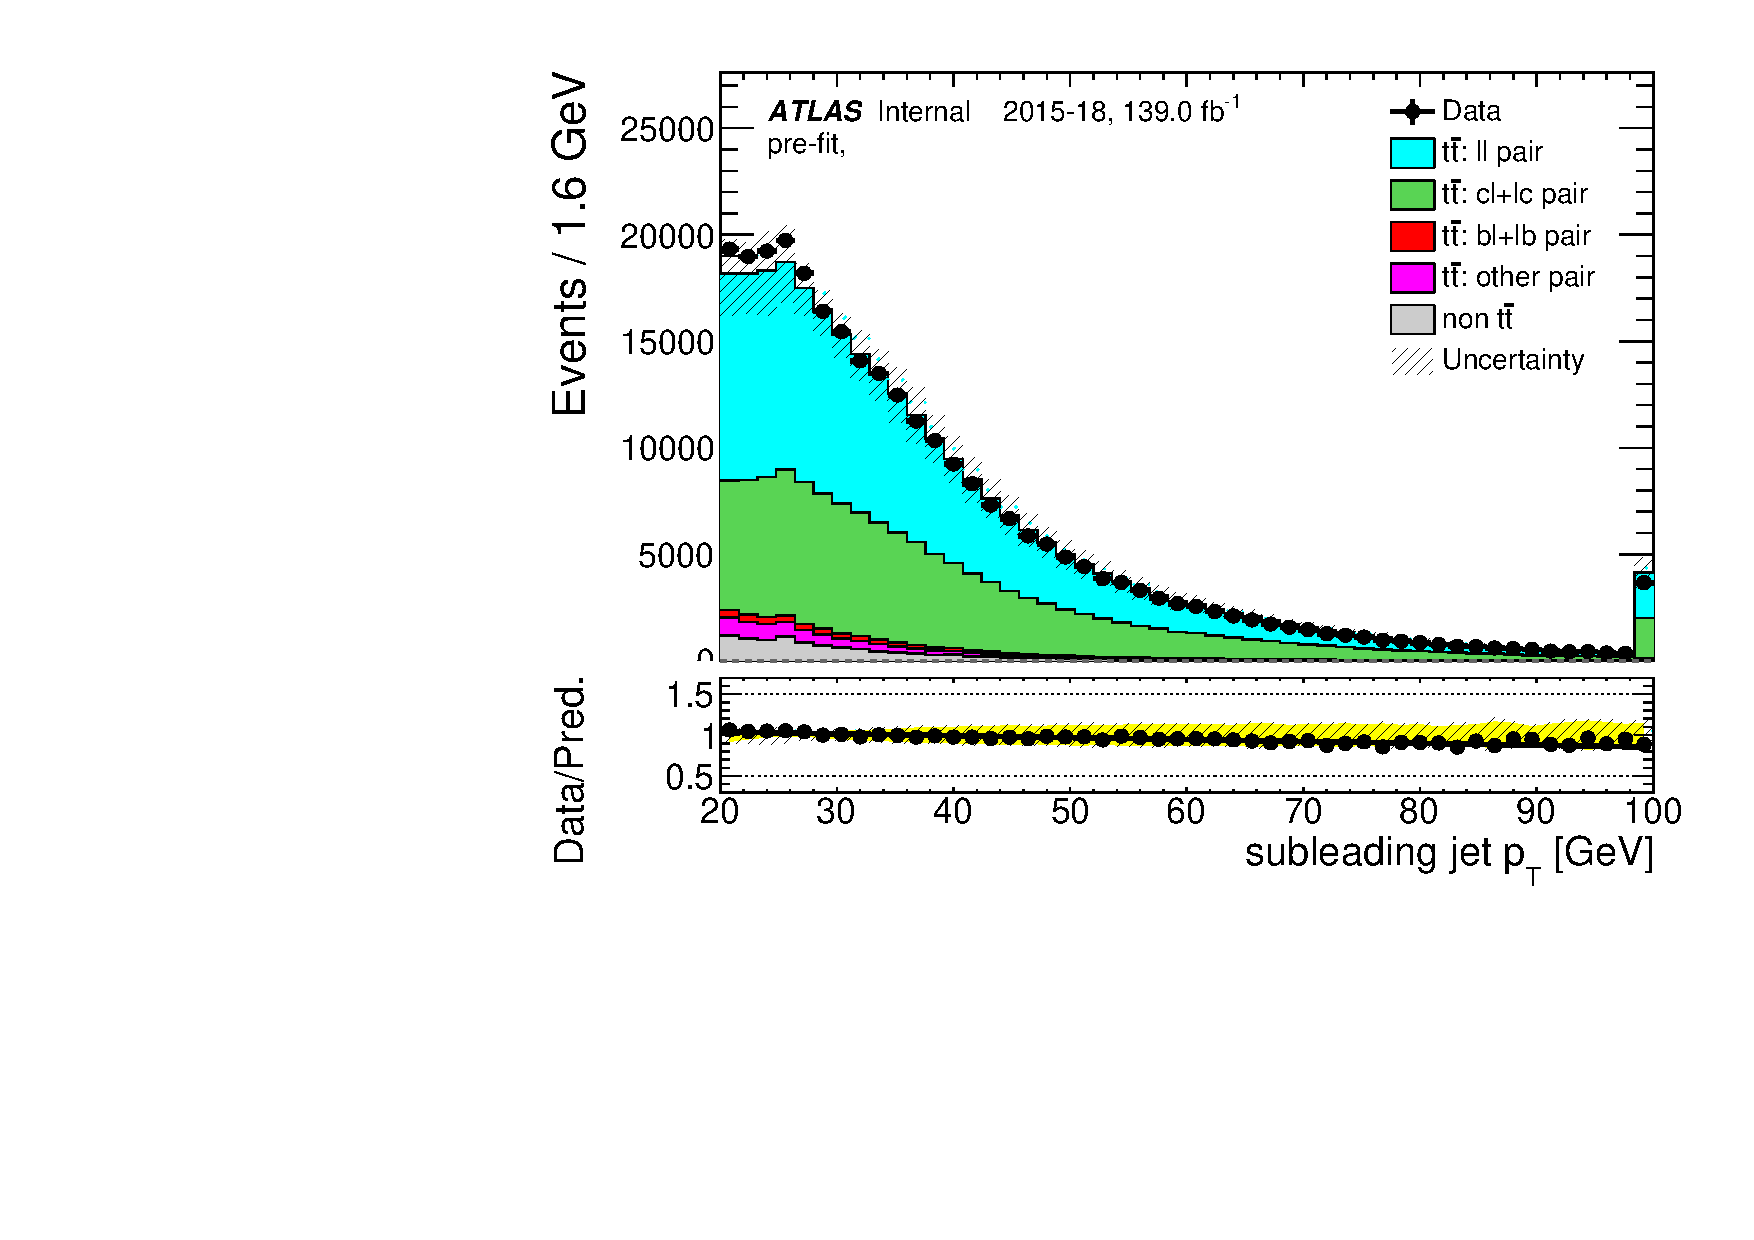
\includegraphics[width=0.45\textwidth]{figs_support/plots_withoutHighpT/DataMC_h_J1_pt.pdf}
	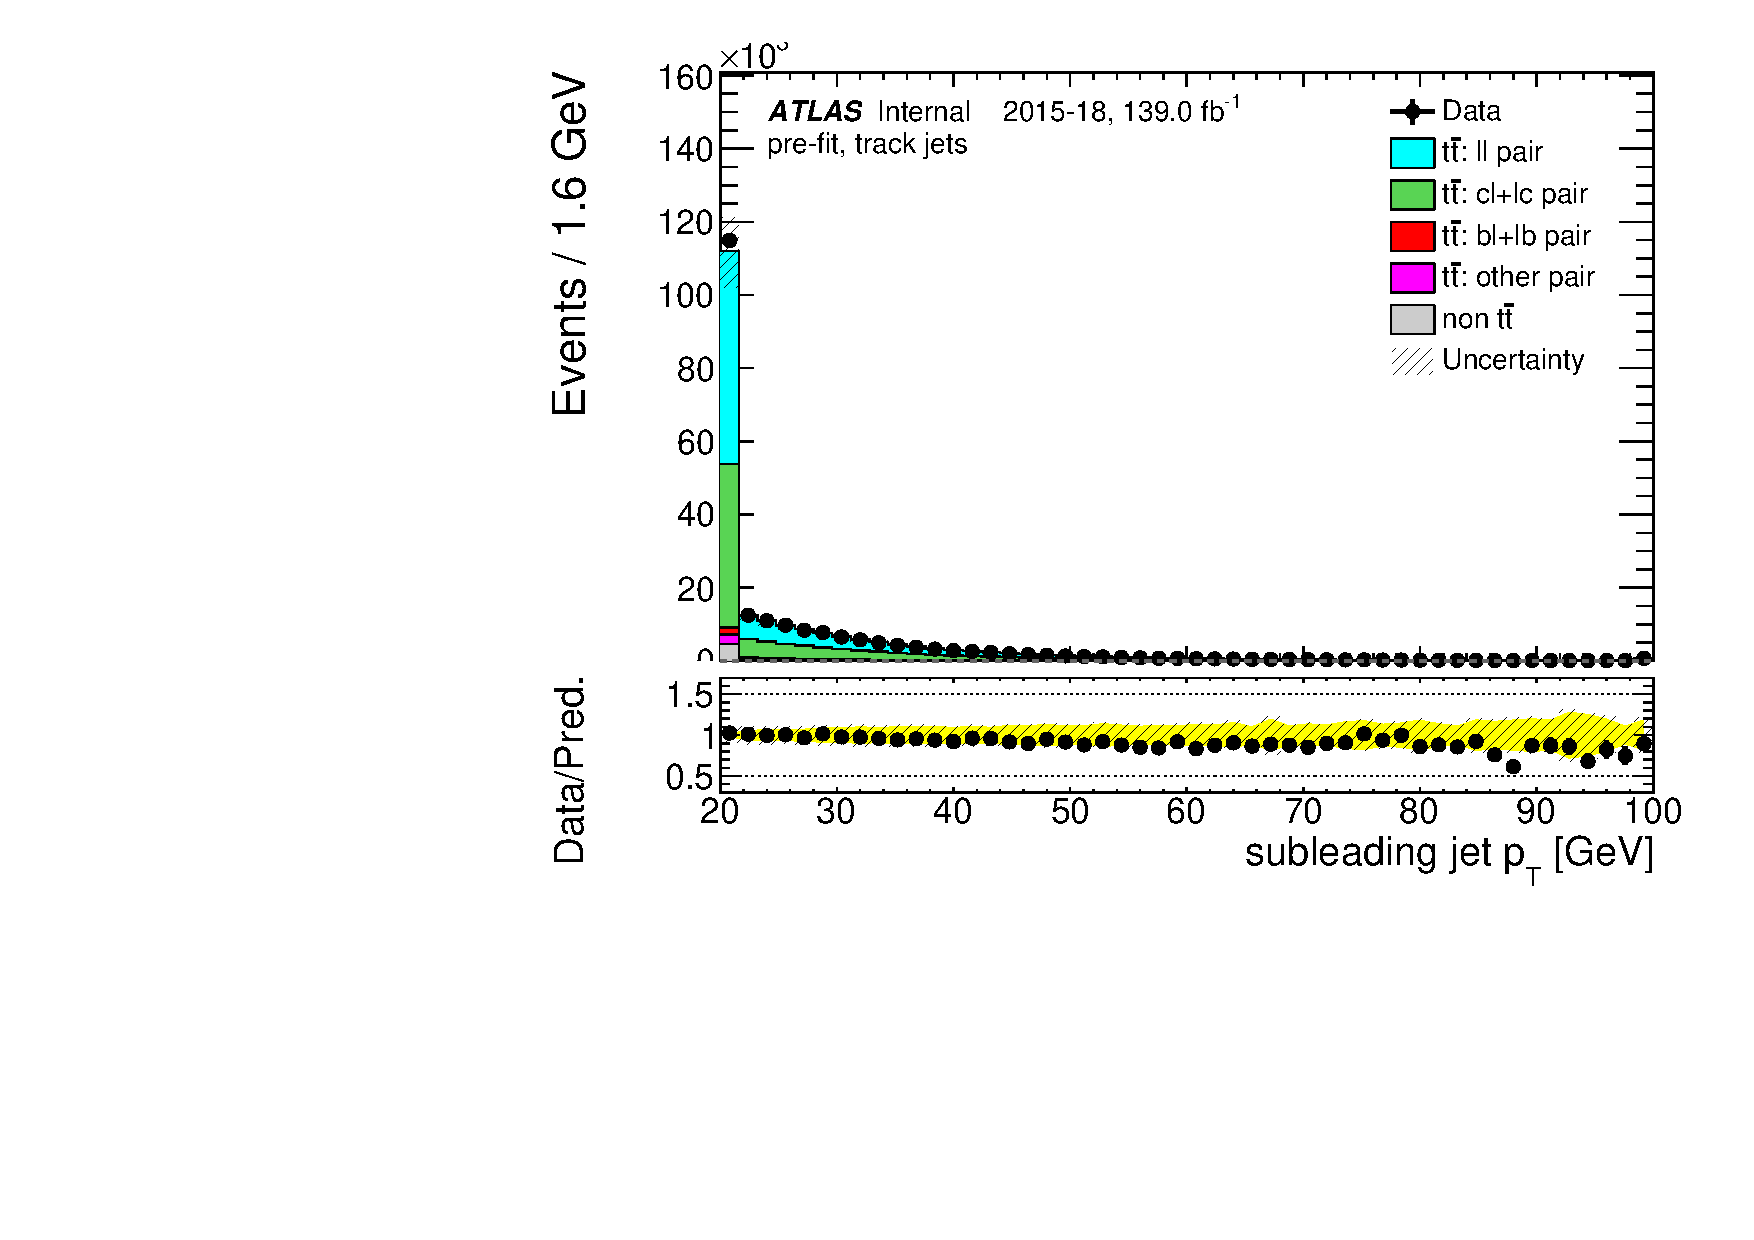
\includegraphics[width=0.45\textwidth]{figs_support/plots_withoutHighpT/DataMC_h_J1_pttrackjet.pdf}\\
	\caption{Data versus simulation for various variables used in the analysis for 
	particle flow jets in the left column and for track jets in the right column.}
	\label{fig:kinematic_distributions_standard}
	\end{figure}
	

\subsubsection{Selection for low-$p_{T}$ extension}
In order to extend the calibration in the low-$p_{T}$ region so that the calibration 
can be applied to jets with $p_{T}$ smaller to 25 GeV, instead of requiring events to 
have exactly 4 jets, events are required to have exactly 3 jets with $p_{T}$ greater 
than 25 GeV and exactly 1 jet with $p_{T}$ greater than 20 GeV. Other than that, 
all other requirements for the selection are the same. The distributions of the sub-leading 
jet are shown in appendix, Figure \ref{fig:lowpT_selection}. Good agreement between MC and data 
is shown in these distributions, and the $p_{T}$ range of the sub-leading has gone down to 20 GeV. 



\subsubsection{High $p_T$ selection}
\label{high_pt_selection}
Instead of requiring events to have exactly 4 jets, events are required to 
have at least 5 jets with $p_{T}$ greater than 25 GeV, in which at least 
1 jet with $p_{T}$ greater than 70 GeV. The choice of cut value is based on 
study shown in the following section \ref{cutvalue}. Other than that, all 
other requirements for the selection remaining the same. 
The yields of the data/MC are given in Table \ref{tab:yields_highpT}, 
an example of the \pt\ distributions before any tagging or fitting and 
after the standard selection is shown in Figure \ref{fig:kinematic_distributions_highpT}. More plots 
can be found in Appendix, Figure \ref{fig:highpT_selection}.

\begin{table}[!b]
	\centering
	\small
	\setlength\tabcolsep{5pt} 
	\begin{tabular}{|l | ll | ll |}
	\hline
	& \multicolumn{2}{c|}{Particle flow jets} & \multicolumn{2}{c|}{Track jets} \\
	\hline
	
	Data    &     98273.0              &   &    120929.0                  &   \\ 
	Ttbar   &     99432.4 $\pm$  116.4 &   &    117090.1 $\pm$      126.5 &    \\
	Other   &      1841.5 $\pm$   21.2 &   &      2641.2 $\pm$       47.6 &    \\
	Data/MC &   0.970 $\pm$ 0.003      &   &      1.010 $\pm$ 0.003       &    \\
	\hline
	% \multicolumn{5}{|c|}{Comparison of \ttbar\ with systematic samples}\\
	% \hline
	% TtbarAF2       &    99325.7 $\pm$   128.7 &  -0.107\%  &   117332.9 $\pm$   140.0 &  0.207\%\\   
	% DATA/MC(AF2)   &  0.971 $\pm$ 0.003       &            &  1.008 $\pm$ 0.003 &      \\            
	% TtbarRadHi     &    97805.0 $\pm$   114.3 & -1.637\%   &   115259.7 $\pm$   124.3  & -1.563\%\\  
	% DATA/MC(RADHI) & 0.986 $\pm$ 0.003        &            & 1.026 $\pm$ 0.003   & \\                
	% TtbarPH        &    99258.1 $\pm$  118.6  & -0.175\%   &   118412.1 $\pm$      130.1  & 1.129\%\\
	% DATA/MC(PH)    & 0.972 $\pm$ 0.003        &            & 0.999 $\pm$ 0.003                   & \\
	  
	% \hline
	\end{tabular}
	\vspace{0.2cm}
	\caption{Prefit comparison of the number of events in data and in 
	simulation considering particle flow jets and track jets for the high-\pt\ 
	selection.}
	\label{tab:yields_highpT}
	\end{table}

\begin{figure}%[htb]
		\centering
		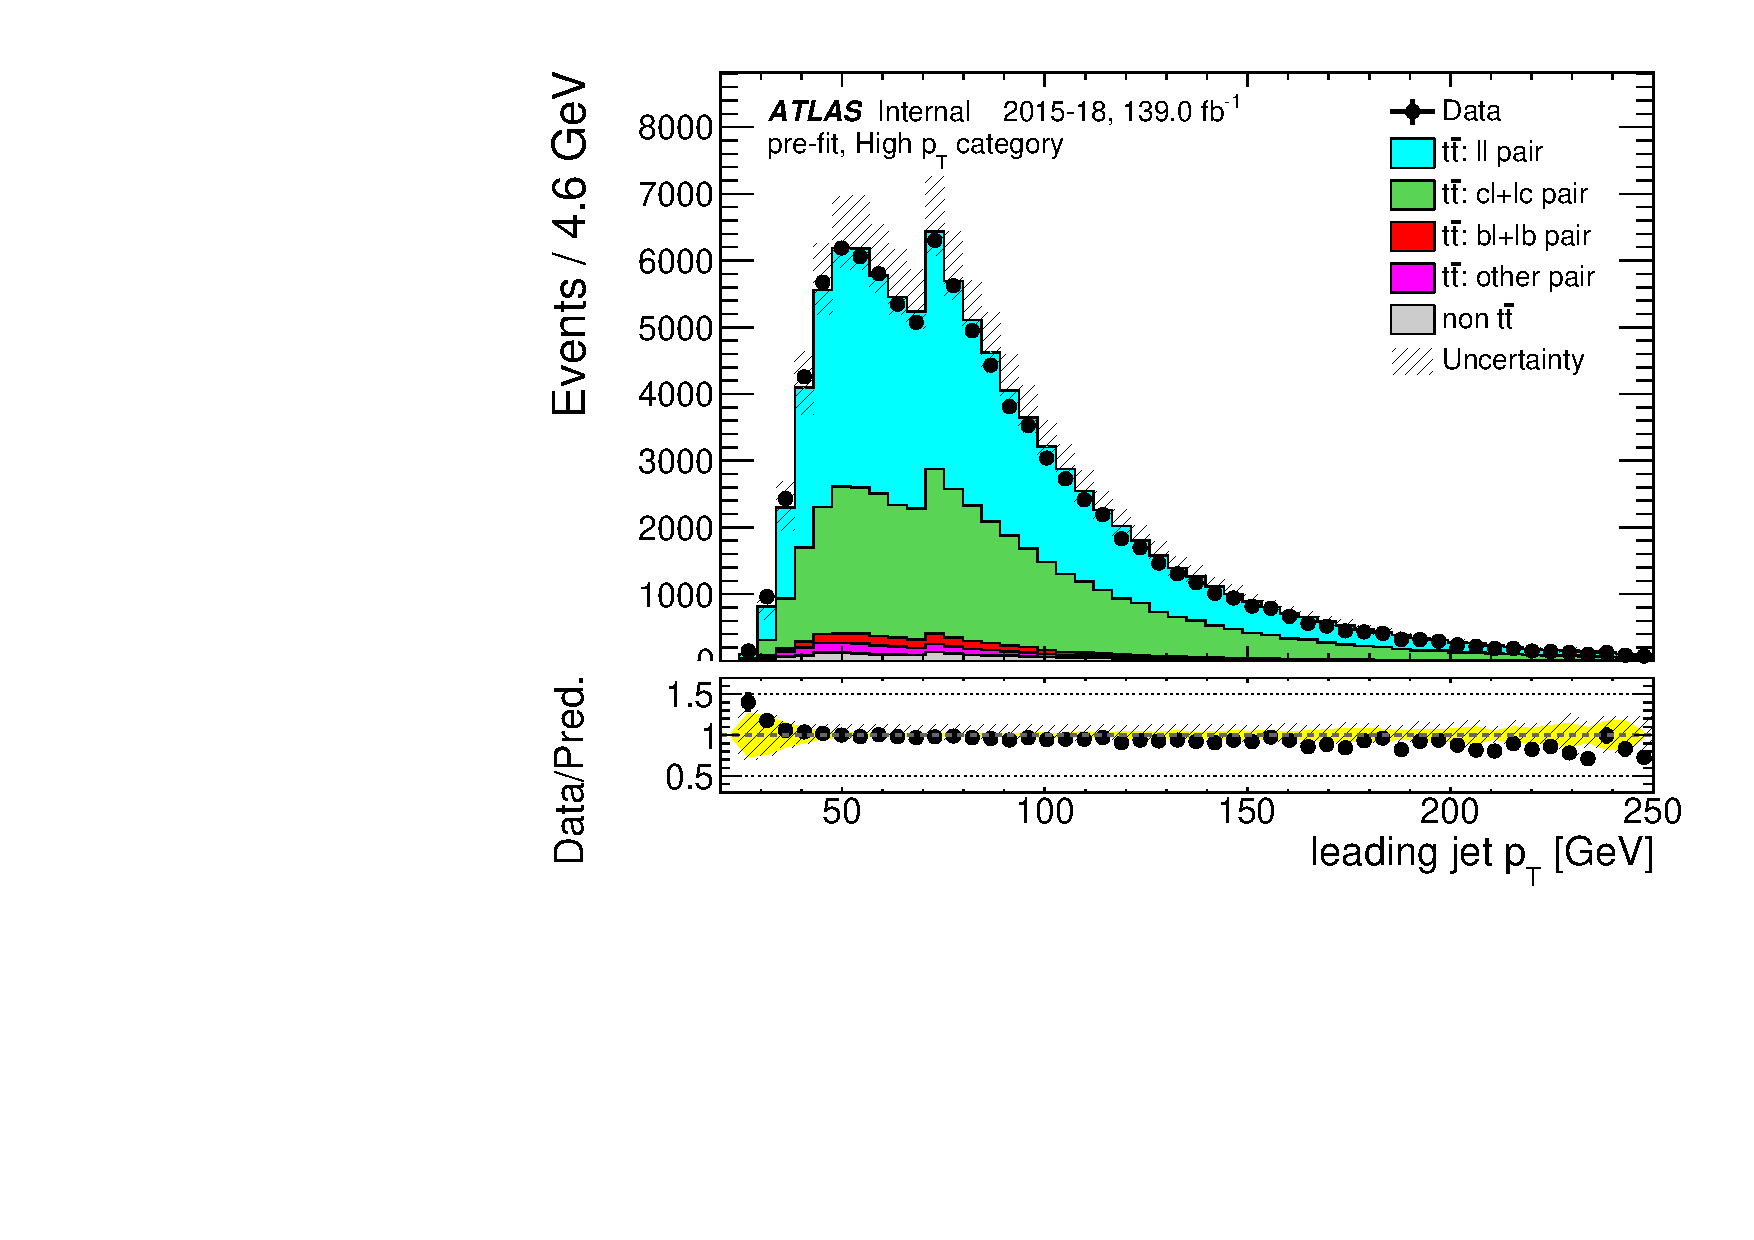
\includegraphics[width=0.45\textwidth]{figs_support/plots_hm/DataMC_h_J0_pt_all_2.pdf}
		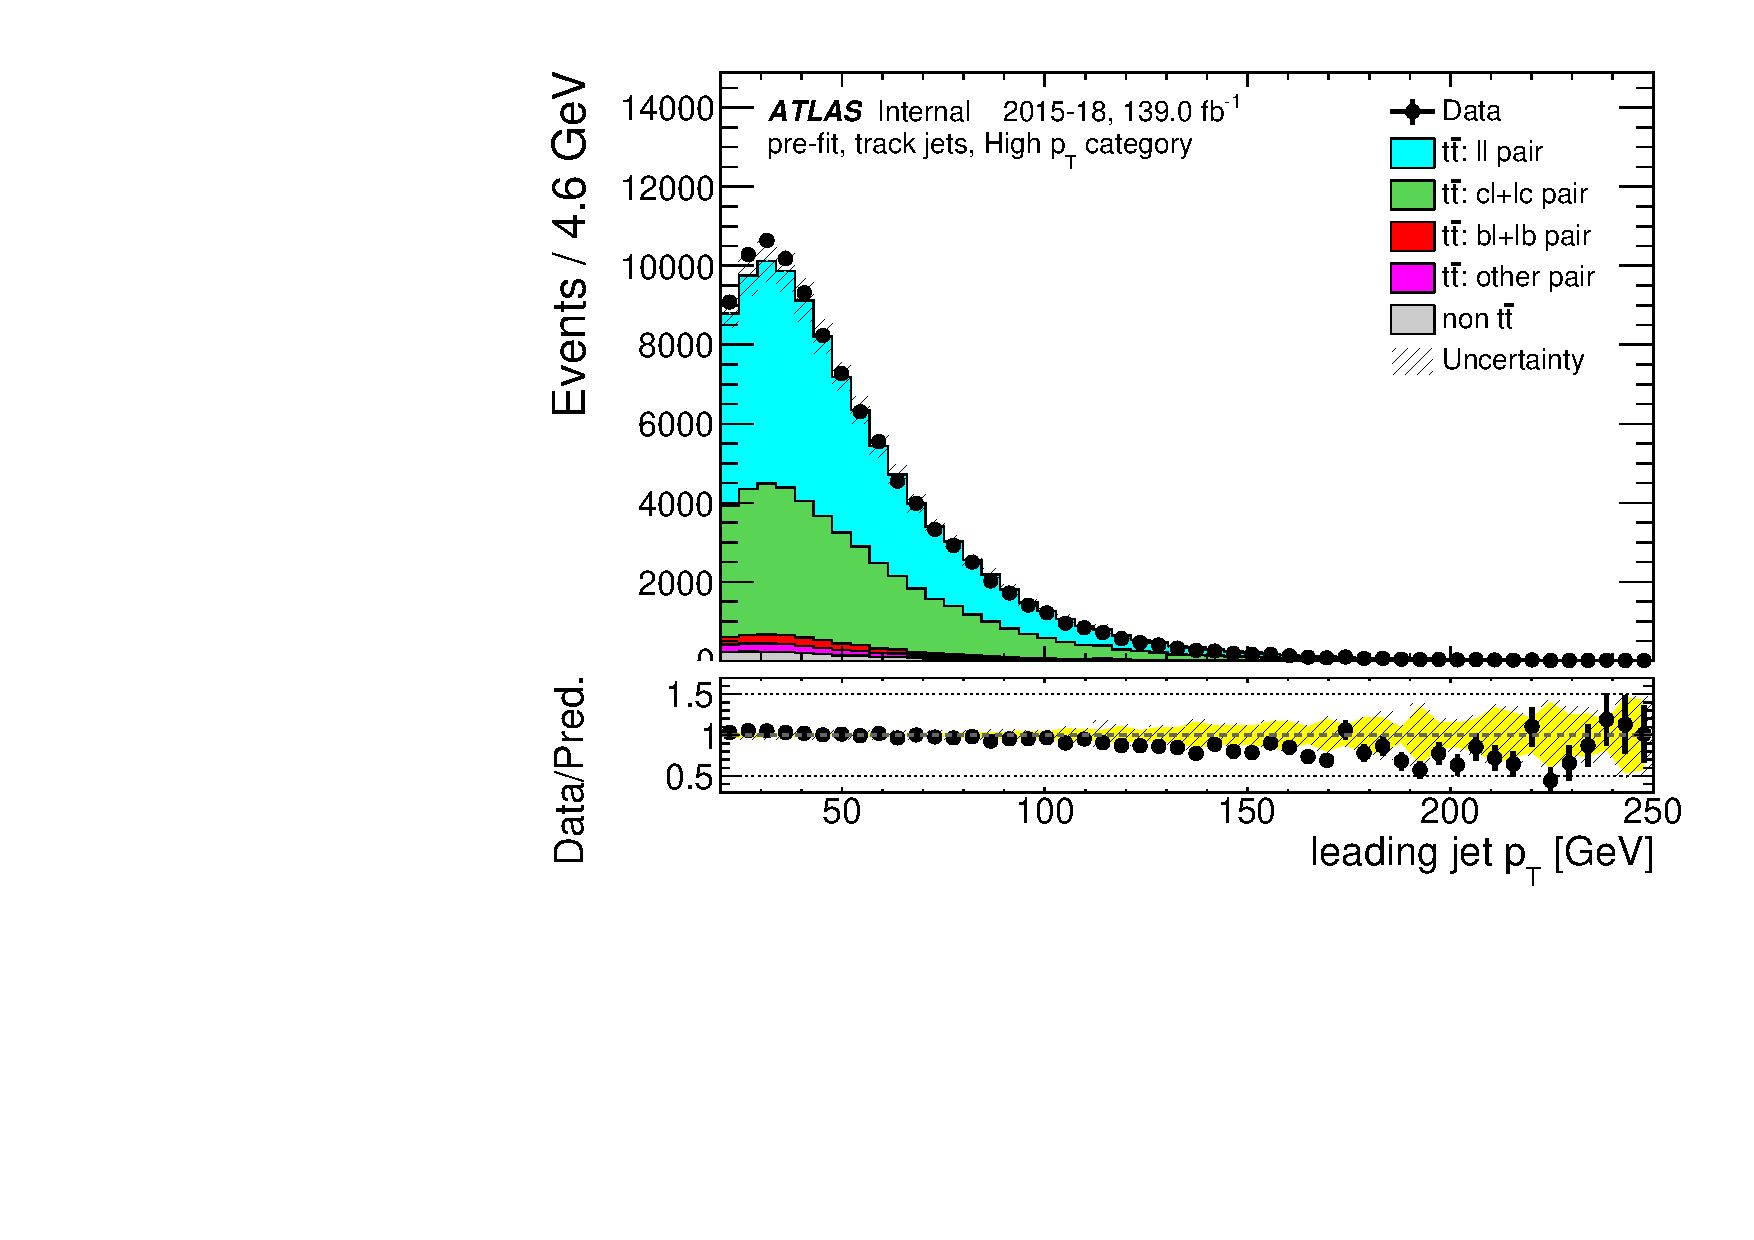
\includegraphics[width=0.45\textwidth]{figs_support/plots_hm/DataMC_h_tjet_J0_pt_all_2.pdf}\\
		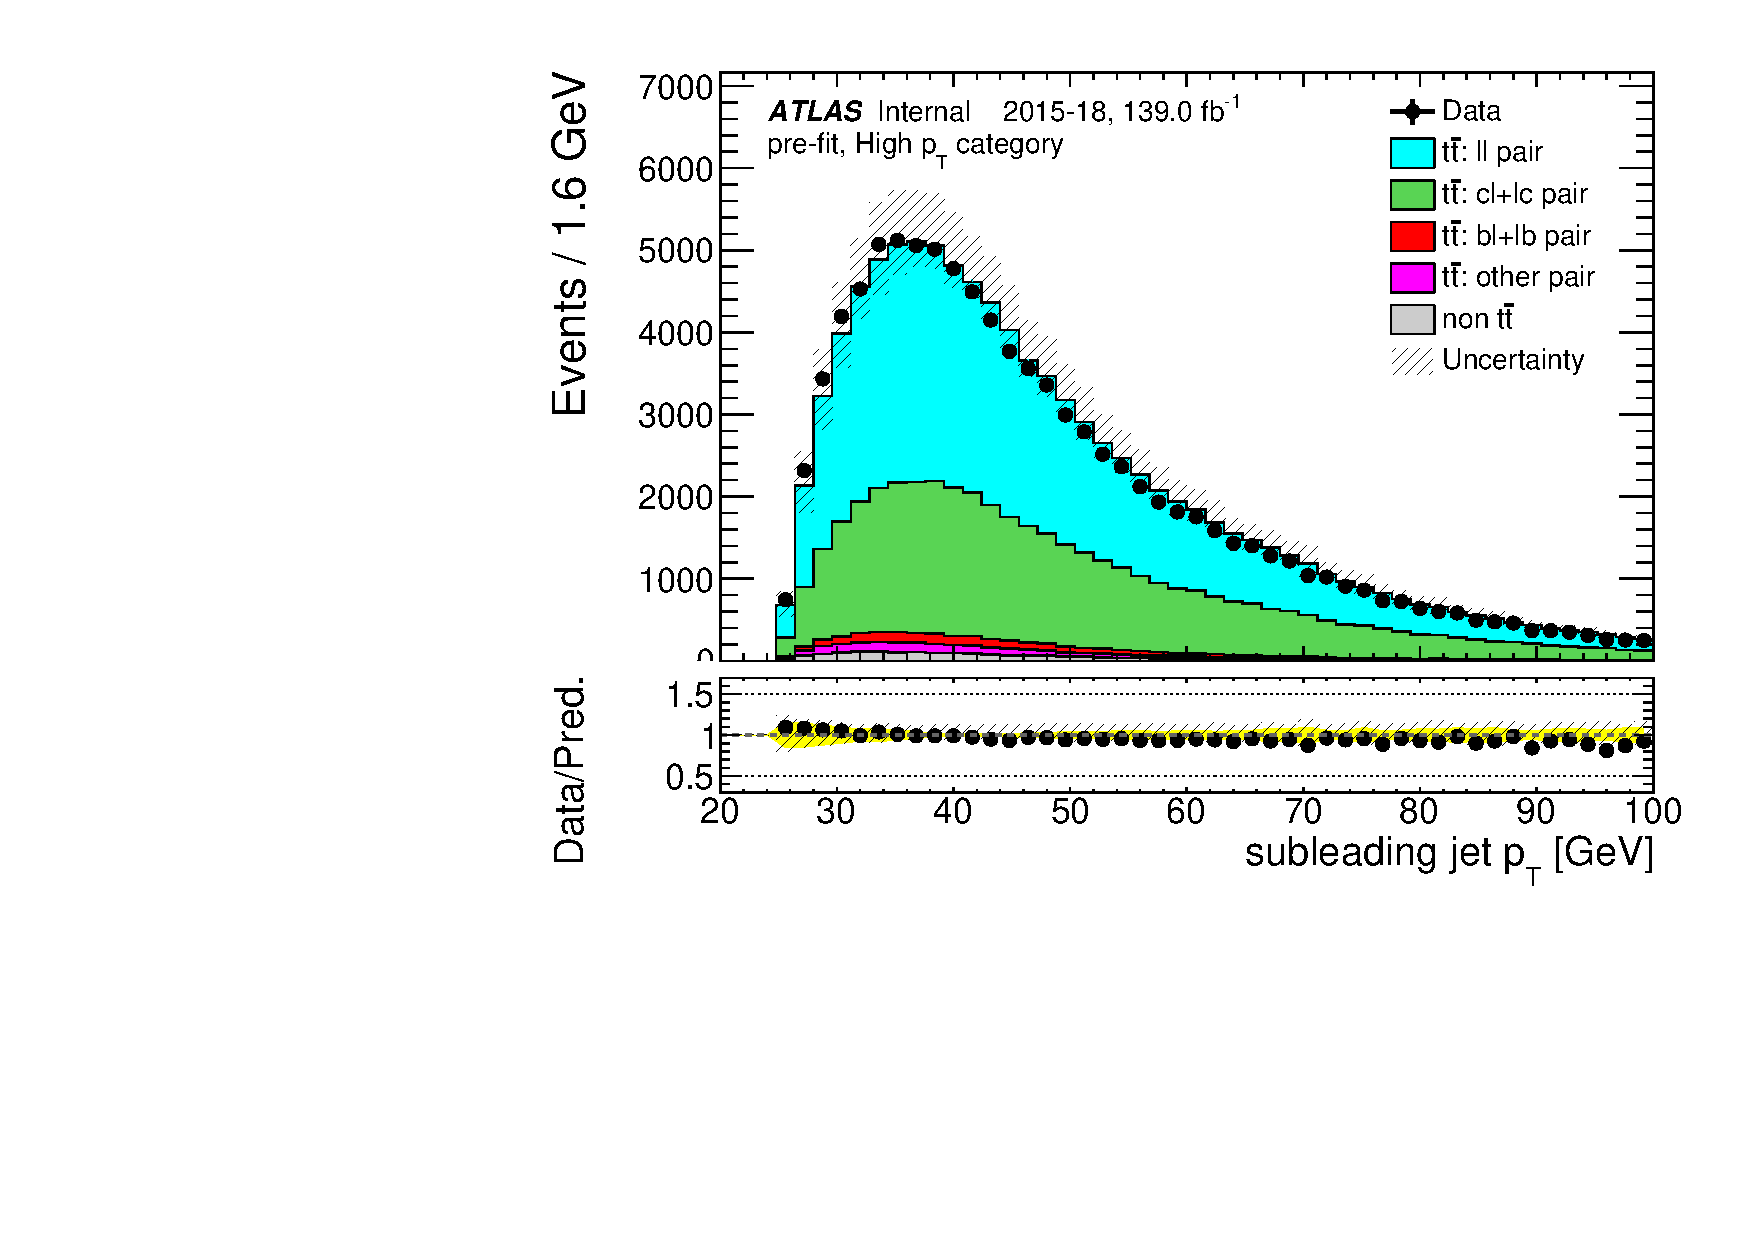
\includegraphics[width=0.45\textwidth]{figs_support/plots_hm/DataMC_h_J1_pt_all_2.pdf}
		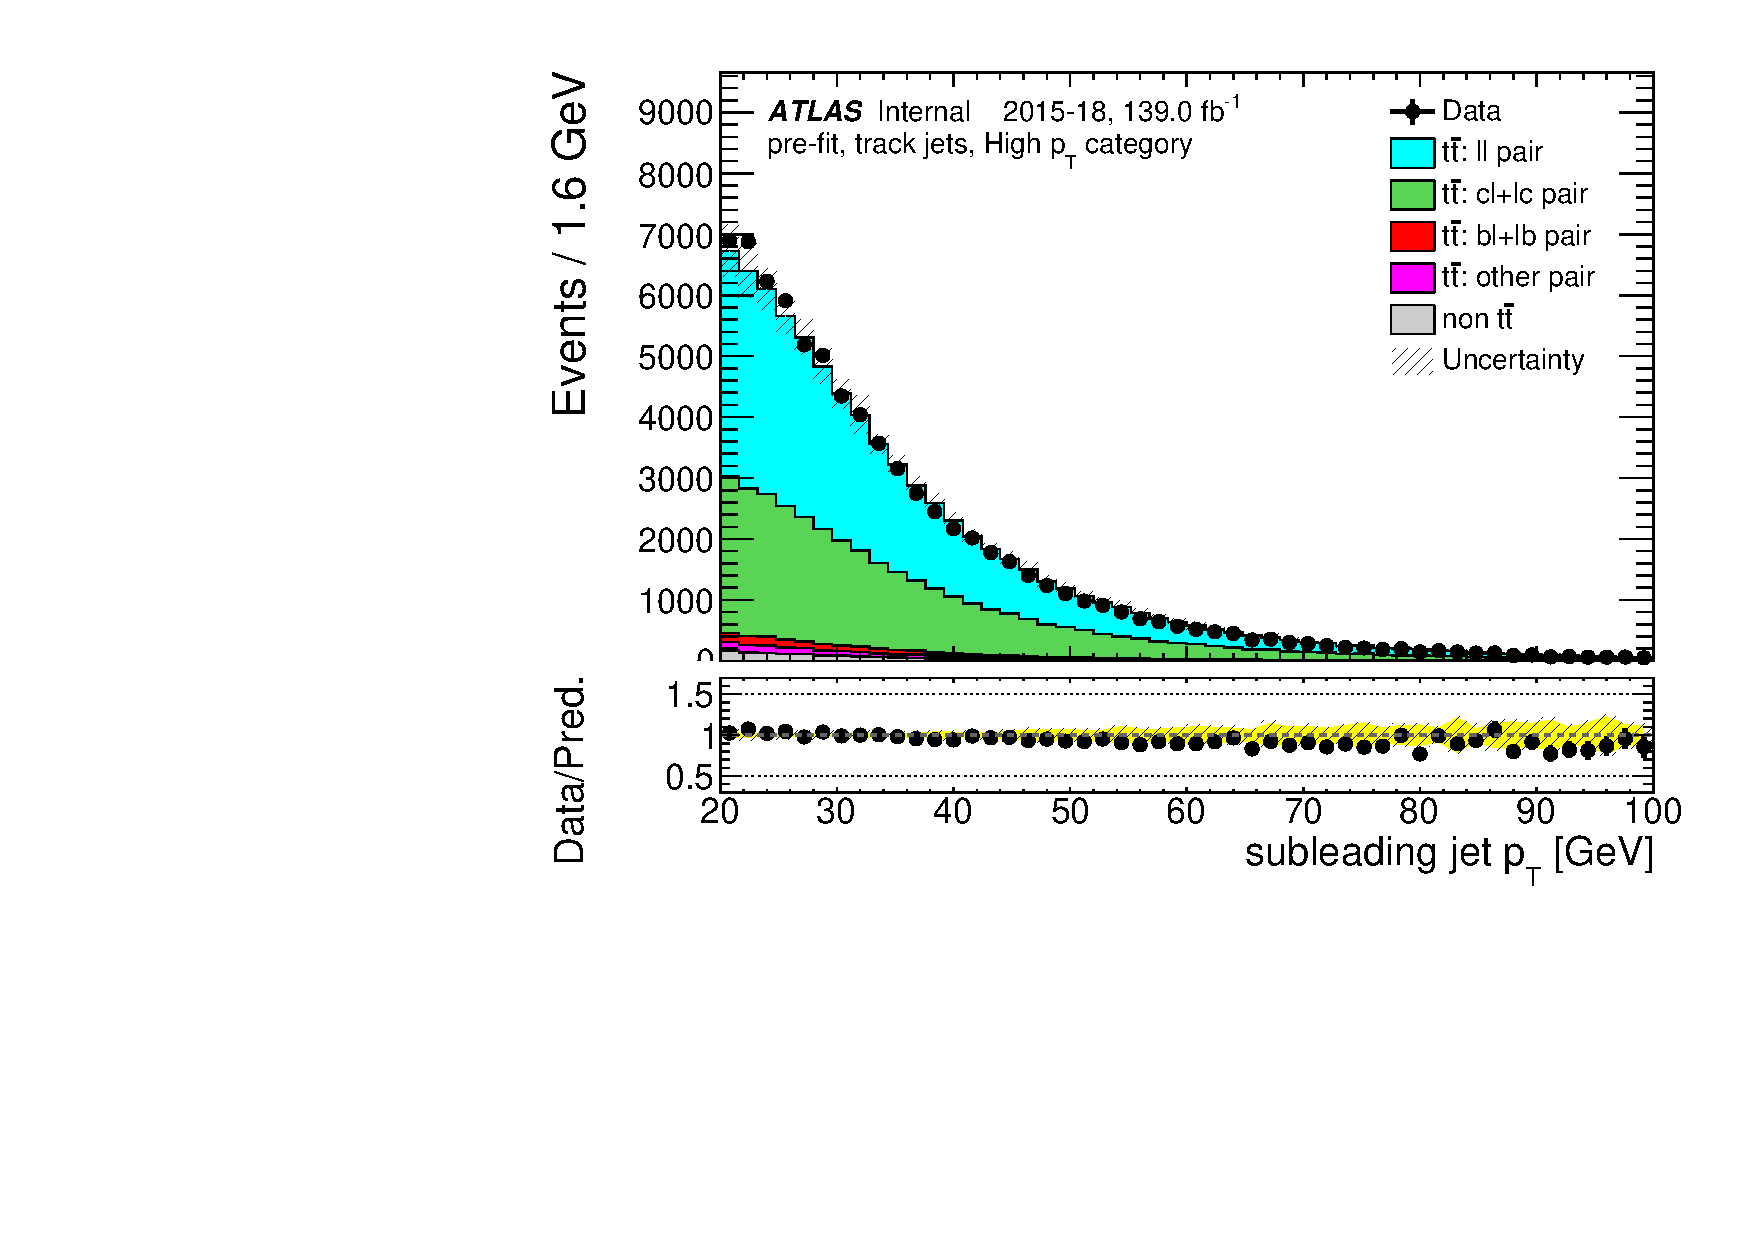
\includegraphics[width=0.45\textwidth]{figs_support/plots_hm/DataMC_h_tjet_J1_pt_all_2.pdf}\\
		\caption{Data versus simulation for various variables used in the analysis for 
		particle flow jets in the left column and for track jets in the right column.}
		\label{fig:kinematic_distributions_highpT}
\end{figure}
		

\paragraph{Optimisation of high $p_{T}$ cut}
\label{cutvalue}

In the high-$p_{T}$ selection, the value to define high-p$_{T}$ is 
chosen to be 70 GeV. A study has been done to investigate the effect 
on the $c$-jet purity and the potential statistical gain, where the $c$-jet purity is defined as:
\begin{equation}
\cjetineq\ purity = \frac{N_{true\ \cjetunder}}{N_{all}},
\end{equation}
where $N_{true\ \cjetunder}$ stands for the number of events with a 
true $c$-jet from the $W$ decay, and $N_{all}$ stands for the number of all events. 
The $c$-jet purity and the statistical gain are calculated for 4 different cut 
values as shown in Figure \ref{fig:cutvalue}, comparing with the cut value of 0. 
The value of 70 GeV is chosen because of its relatively small effect on the $c$-jet 
purity and relatively high gain in statistics. 


\begin{figure}
\begin{minipage}[b]{.45\textwidth}
\centering
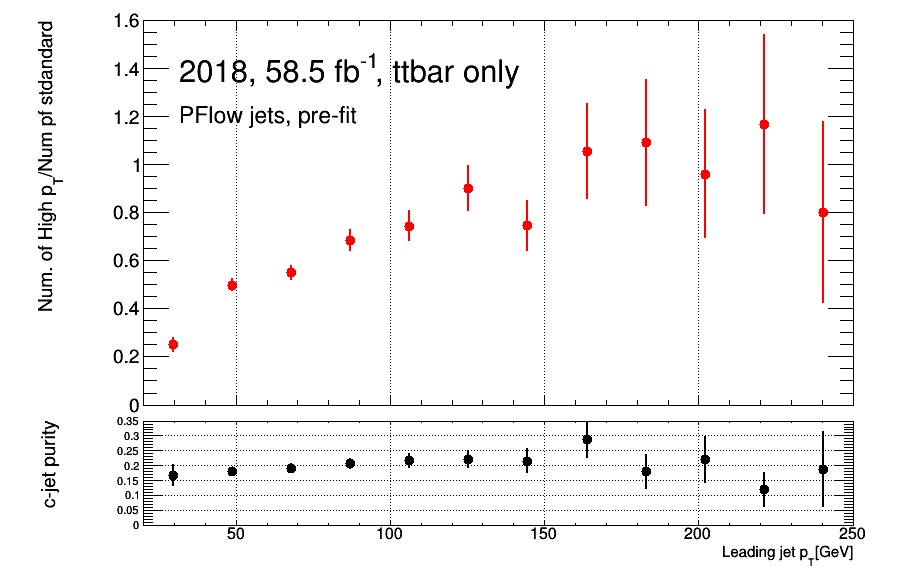
\includegraphics[width=1\textwidth]{stat_gains/statsgain_0GeV.png}
\footnotesize (a) Gain in stats and the $c$-jet purity with cut value 0 GeV.
\end{minipage}\hfill
\begin{minipage}[b]{.45\textwidth}
\centering
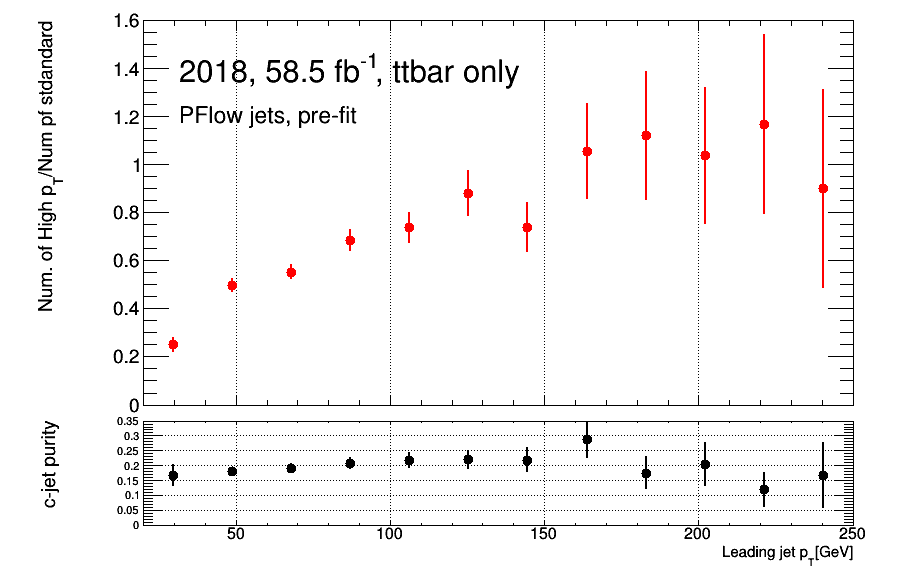
\includegraphics[width=1\textwidth]{stat_gains/statsgain_40GeV.png}
\footnotesize (b) Gain in stats and the $c$-jet purity with cut value 40 GeV.
\end{minipage}\hfill
\begin{minipage}[b]{.45\textwidth}
\centering
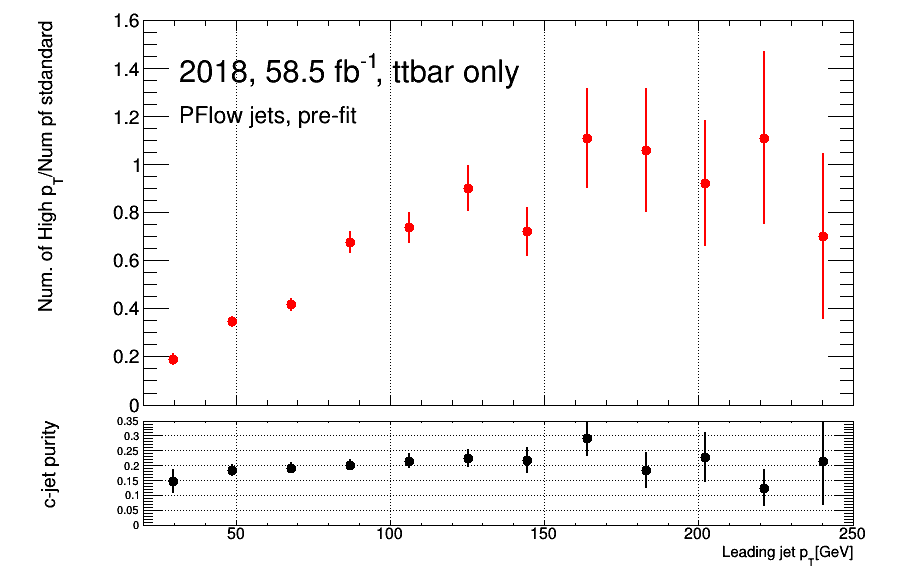
\includegraphics[width=1\textwidth]{stat_gains/statsgain_70GeV.png}
\footnotesize (c) Gain in stats and the $c$-jet purity with cut value 70 GeV.
\end{minipage}\hfill
\begin{minipage}[b]{.45\textwidth}
\centering
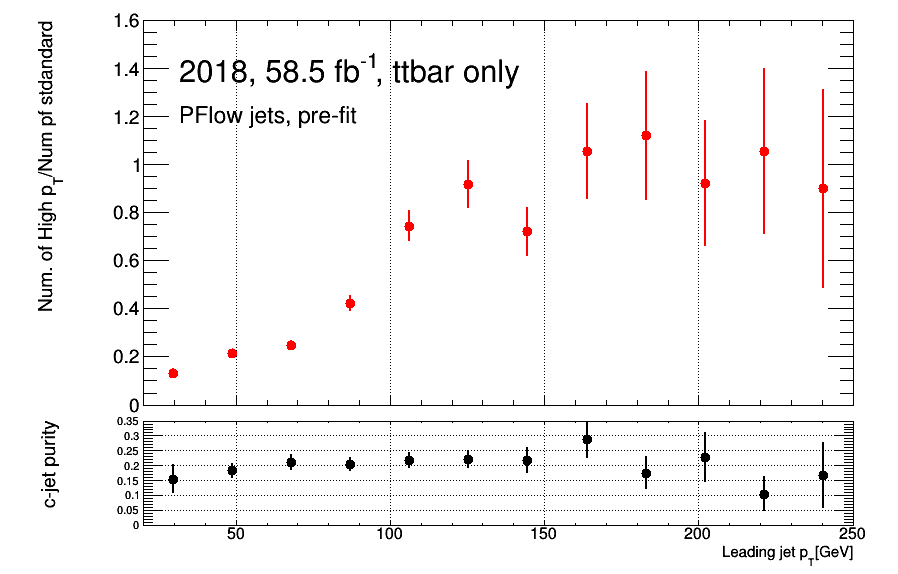
\includegraphics[width=1\textwidth]{stat_gains/statsgain_90GeV.png}
\footnotesize (c) Gain in stats and the $c$-jet purity with cut value 90 GeV.
\end{minipage}\hfill
\begin{minipage}[b]{.45\textwidth}
\centering
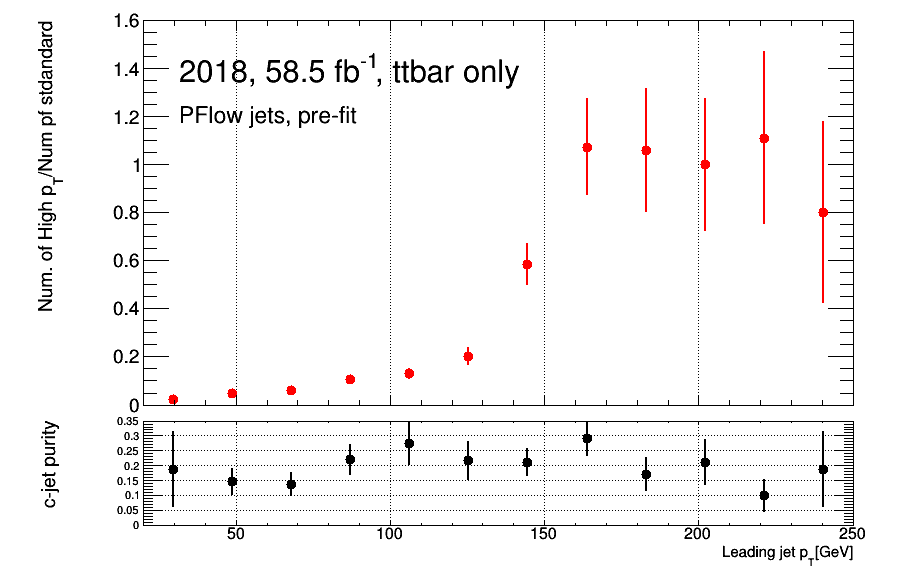
\includegraphics[width=1\textwidth]{stat_gains/statsgain_140GeV.png}
\footnotesize (d) Gain in stats and the $c$-jet purity with cut value 140 GeV.
\end{minipage}\hfill

\caption{Comparison of different cut values in terms of gain in stats and $c$-jet purity.}
\label{fig:cutvalue}
\end{figure}


\subsubsection{Combined selection}
\label{combined_selection}
As the standard selections, low \pt\ selection and high \pt\ selection are othorgonal 
to each other, all the selections are combined to provide the maximum range 
and statistics for the calibration. 
The yields of the data/MC are given in Table \ref{tab:yields_combined}, 
an example of the \pt\ distributions before any tagging or fitting and 
after the standard selection is shown in Figure \ref{fig:kinematic_distributions_combined}. More plots 
can be found in Appendix, Figure \ref{fig:jets_PFlow,fig:angles_PFlow,fig:mass_PFlow,
fig:jets_VRJets, fig:angles_VRJets, fig:mass_VRJets, fig:combined_selection}.
\begin{table}[!b]
	\centering
	\small
	\setlength\tabcolsep{5pt} 
	\begin{tabular}{|l | ll | ll |}
	\hline
	& \multicolumn{2}{c|}{Particle flow jets} & \multicolumn{2}{c|}{Track jets} \\
	\hline
	Data          &    385378.0                  &        &   302308.0              &     \\  
	Ttbar         &    383517.0 $\pm$      229.4 &        &   302690.5 $\pm$      203.9 &   \\
	Other         &     12424.0 $\pm$      123.8 &        &     8566.8 $\pm$      104.1 &   \\
	Data/MC       &    0.973 $\pm$ 0.002         &        &  0.971 $\pm$ 0.002  &           \\
	\hline
	% \multicolumn{5}{|c|}{Comparison of \ttbar\ with systematic samples}\\
	% \hline
	% TtbarAF2       &   386261.9 $\pm$ 254.5  &  0.716\% & 304858.1 $\pm$ 226.1 &  0.716\%\\
	% DATA/MC(AF2)   &   0.967 $\pm$ 0.002     &      & 0.965 $\pm$ 0.002 &      \\              
	% TtbarRadHi     &   377129.7 $\pm$   224.0  & -1.665\% &  297963.8 $\pm$   200.3  & -1.562\%\\     
	% DATA/MC(RADHI) & 0.989 $\pm$ 0.002         &      & 0.986 $\pm$ 0.002   &  \\       
	% TtbarPH        &   331961.5 $\pm$   217.0  & -13.443\%&  259942.3 $\pm$      193.4  & -14.123\%\\ 
	% DATA/MC(PH)    & 1.119 $\pm$ 0.002         &       & 1.126 $\pm$ 0.002     &\\                
	% \hline
	\end{tabular}
	\vspace{0.2cm}
	\caption{Prefit comparison of the  number of events in data and in 
	simulation considering particle flow jets and track jets for an inclusive
	selection.}
	\label{tab:yields_combined}
	\end{table}

\begin{figure}%[htb]
		\centering
		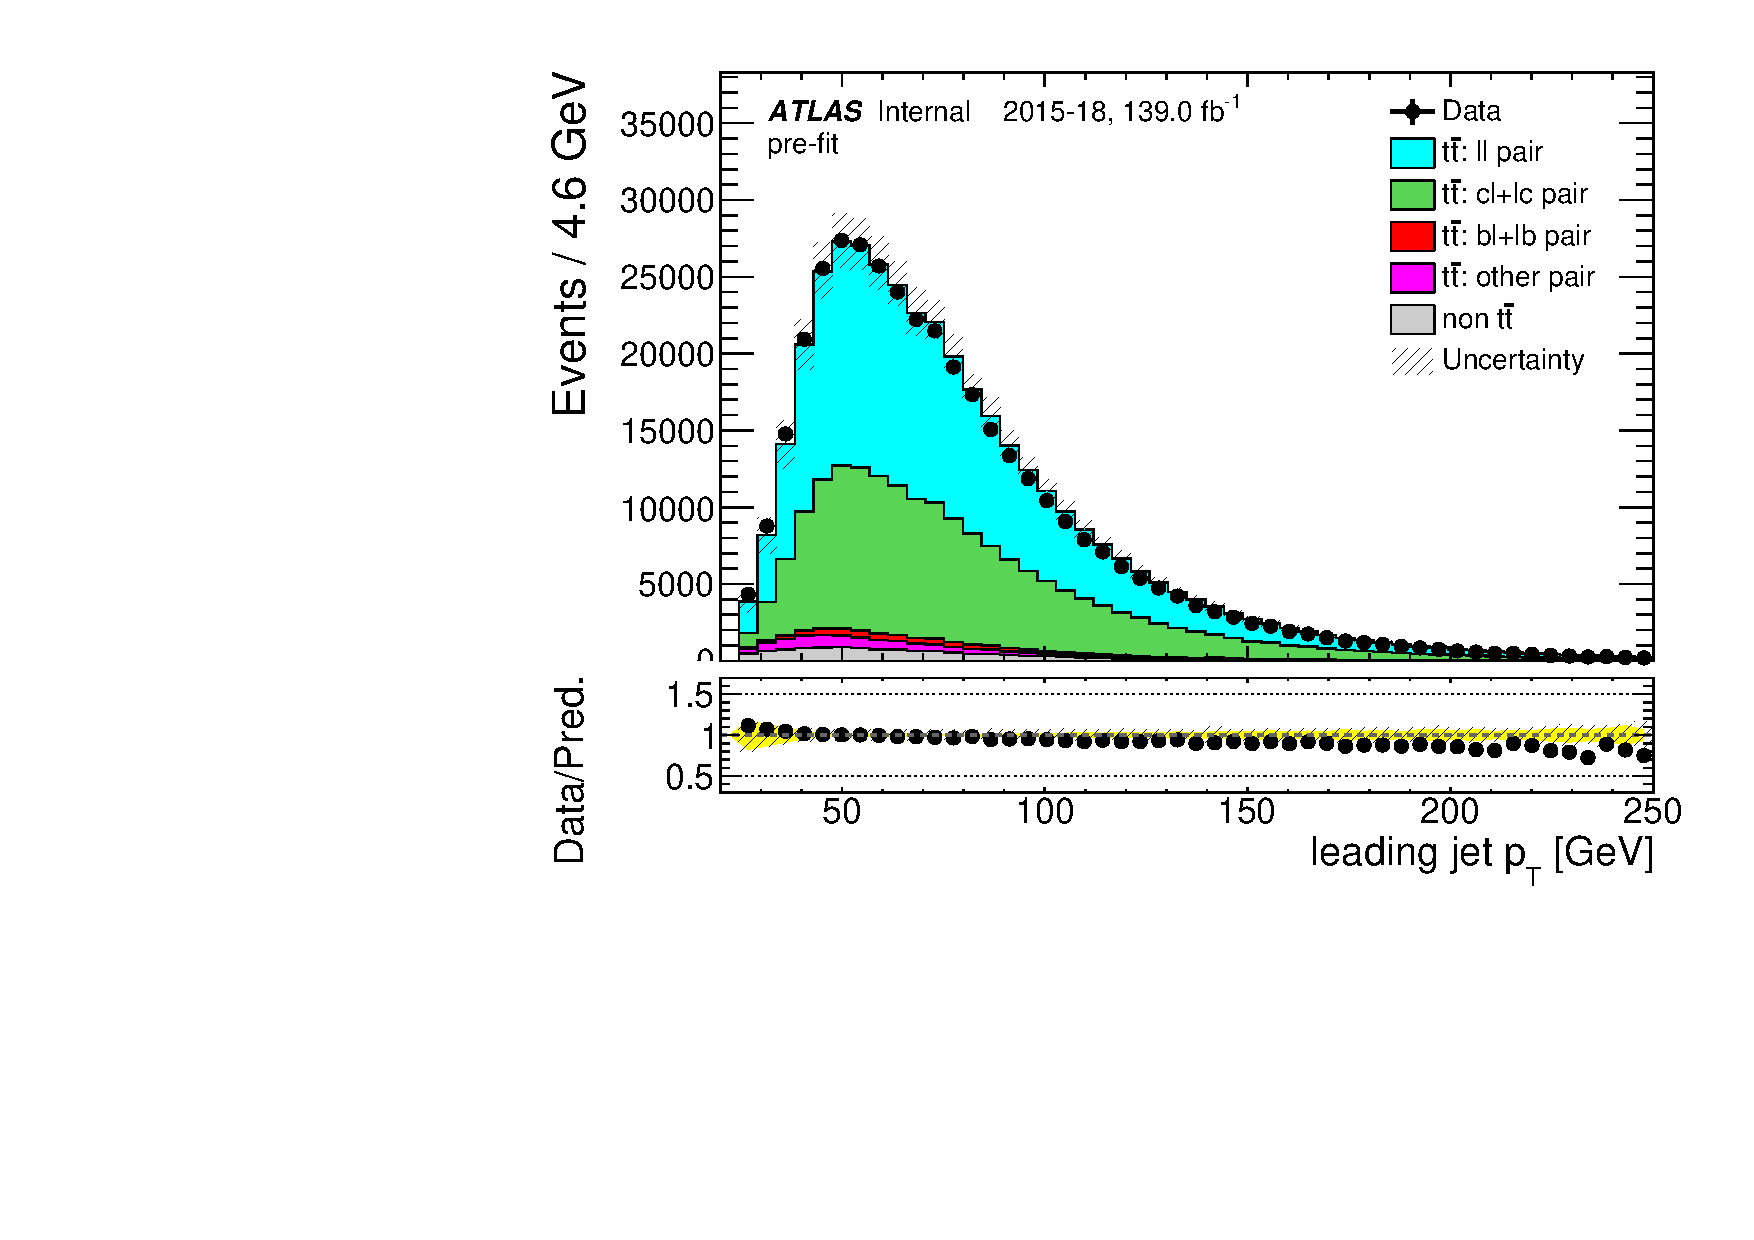
\includegraphics[width=0.45\textwidth]{figs_support/plots_def/DataMC_h_J0_pt_all.pdf}
		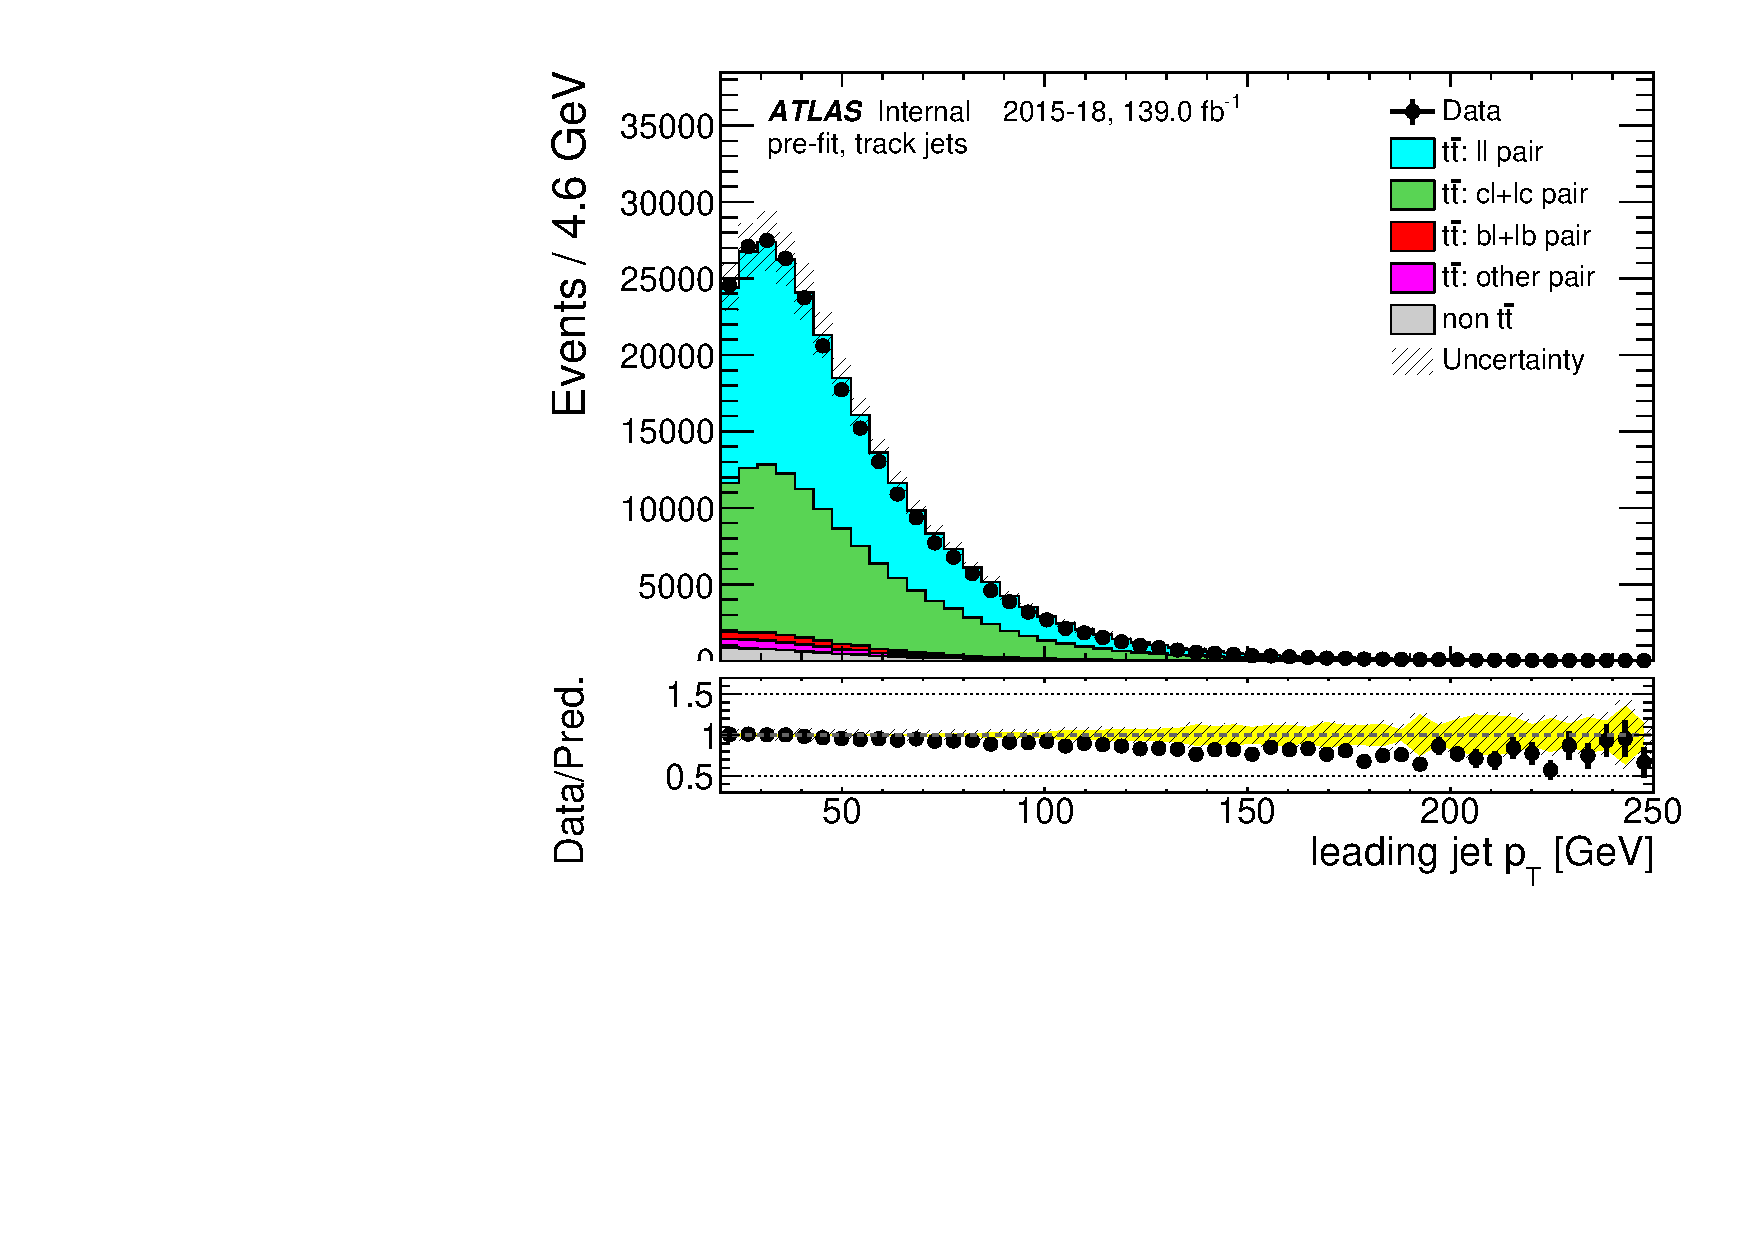
\includegraphics[width=0.45\textwidth]{figs_support/plots_def/DataMC_h_tjet_J0_pt_all.pdf}\\
		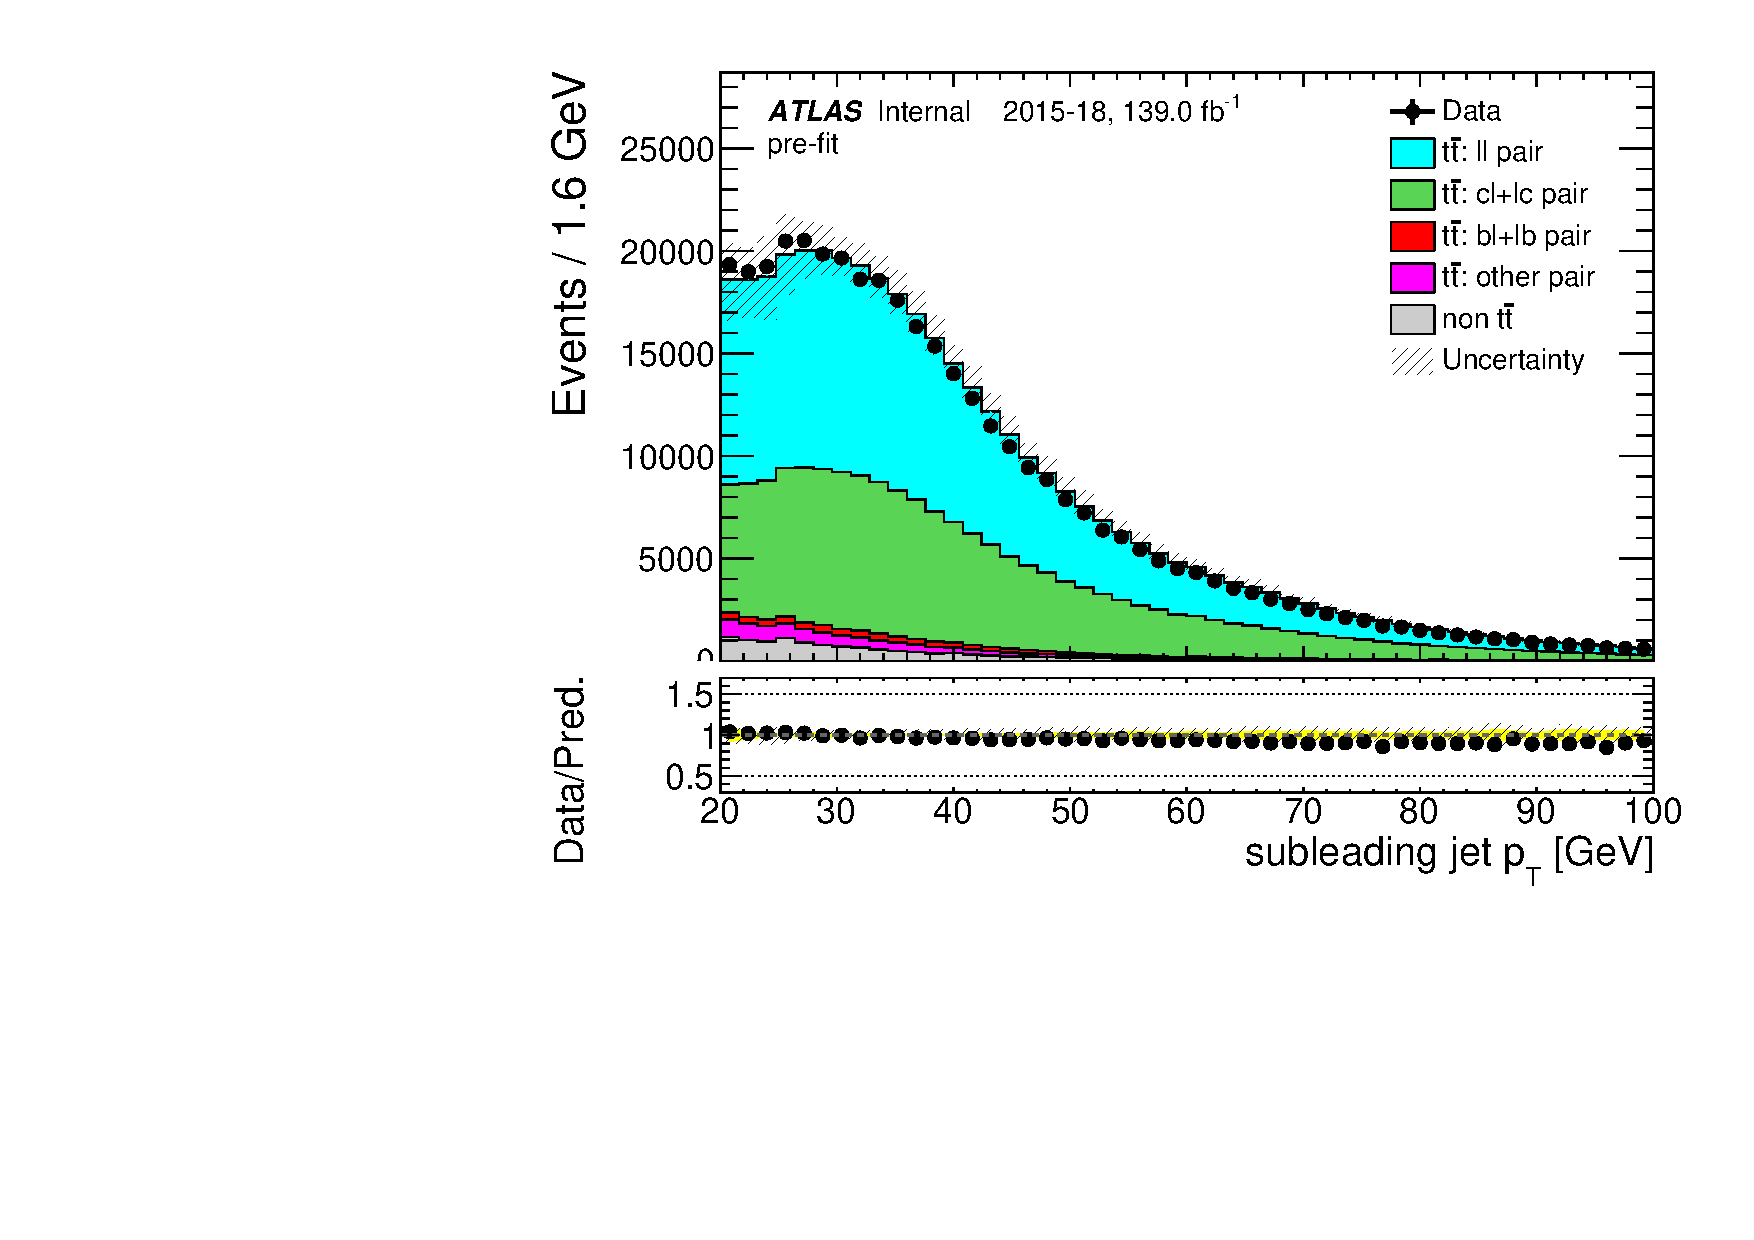
\includegraphics[width=0.45\textwidth]{figs_support/plots_def/DataMC_h_J1_pt_all.pdf}
		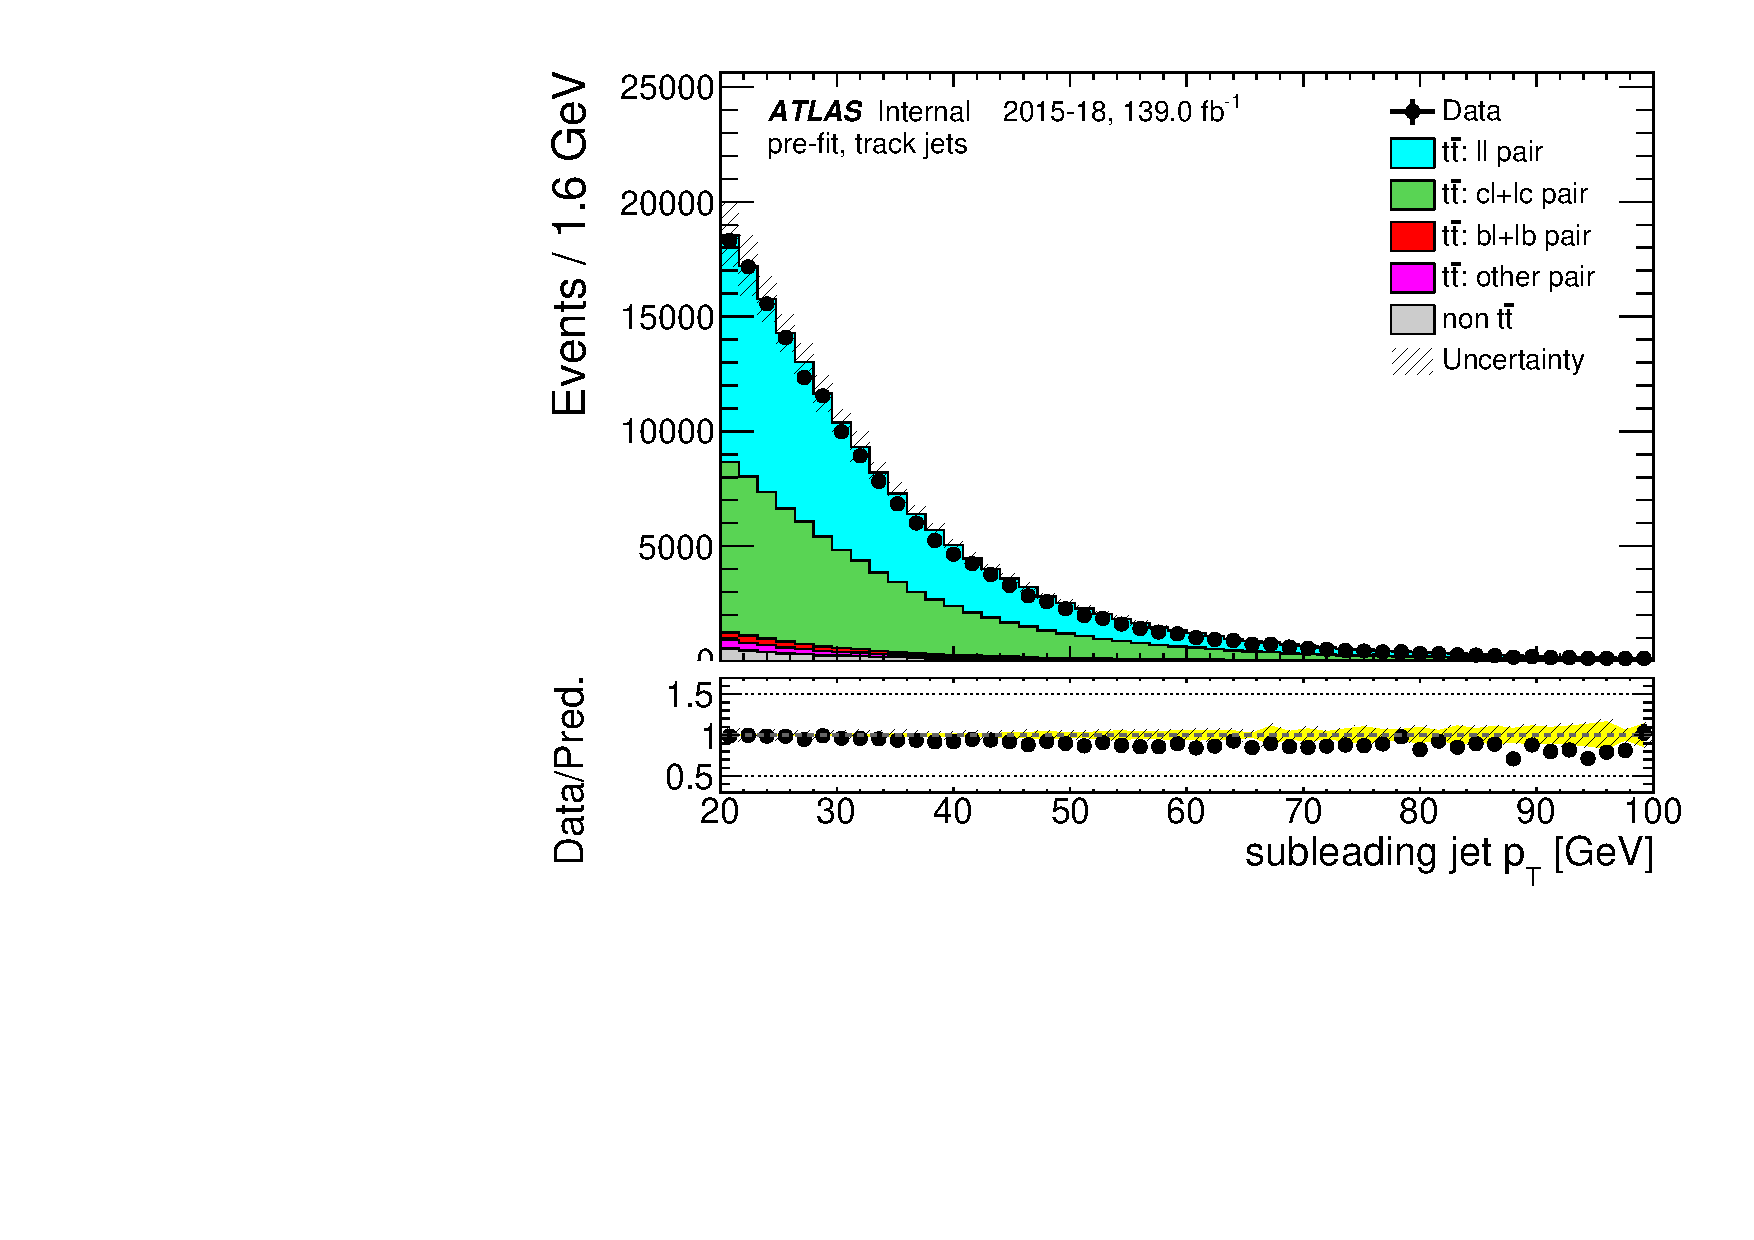
\includegraphics[width=0.45\textwidth]{figs_support/plots_def/DataMC_h_tjet_J1_pt_all.pdf}\\
		\caption{Data versus simulation for various variables used in the analysis for 
		particle flow jets in the left column and for track jets in the right column.}
		\label{fig:kinematic_distributions_combined}
\end{figure}
		

\subsection{Systematic uncertainties}
\label{systematic uncertainties}
The systematic uncertainties considered and propagated in this calibration 
can be broadly categorised into experimental systematics and modelling uncertainties. 
Supporting material for this section can be found in the appendix, Tab.\ref{tab:systematics}.
\subsubsection{Experimental uncertainties}

Experimental uncertainties are related to the detector and estimated using 
data-driven methos or MC simulations. 
The electron energy scale and resolution are corrected to 
provide better agreement between MC predictions and data, uncertainties 
due the corrections are considered. Uncertainties are taken into account the 
electron trigger, identification and reconstruction efficiencies, and for 
uncertainties associated with the isolation requirements. Scaling and smearing 
corrections are applied to the $p_T$ of simulated muons in order to minimise the differences 
in resolution between data and MC events, and the uncertainties of the corrections are considered. 
Differences in the identification efficiency and in the efficiency of the trigger selection are 
also taken into account. The jet energy scale (JES) uncertainty depends on $p_T$ and $\eta$ and 
takes into account uncertainties due to pile-up effects. Uncertainties on the jet energy resolution (JER) 
is taken into account. Uncertainties on the energy scale and resolution of 
the electrons, muons, jets and taus are propagated to the calculation of the $E_T^{miss}$, 
which also has additional dedicated uncertainties on the scale, resolution, and 
reconstruction efficiency of tracks not associated to any of the reconstructed objects,
 along with the modelling of the underlying event. Uncertainties on the $b$-tagging probabilities 
 for $b$- and light-jets are considered both for the tagging jets assigned to the $b$-quark 
 from top decay and for the jets associated to the hadronically decaying $W$ boson.
%The uncertainty on these corrections is taken into account as a shape-dependent systematic uncertainty in the final fit of the backgrounds and signal models.

\subsubsection{Modelling uncertainties} Uncertainties on the modelling of the inclusive $t\bar{t}$ 
background are estimated by replacing the nominal MC sample by alternative MC samples. The nominal 
sample is also replaced by variations of the matrix element generator, parton shower, and initial 
and final state radiation. In all cases, MC-to-MC SFs are taken into account. The uncertainty in 
the choice of NLO matrix element generator is derived by comparing two alternative predictions, 
{\tt POWHEG} and {\tt aMC@NLO\_MG5}, each of which is showered with {\tt HERWIG++}. An uncertainty 
due to the choice of parton shower and hadronisation model is derived by comparing the prediction 
from {\tt POWHEG} interfaced either to {\tt PYTHIA8} or {\tt HERWIG++}. Finally, the uncertainty on 
modelling of initial and final state radiation is assessed with two alternative {\tt POWHEG+PYTHIA8} 
samples. The samples include one with an increase in radiation which has the re-normalisation and 
factorisation scales decreased by a factor of two and the \textit{hdamp} parameter doubled, while 
the sample with a decrease in radiation has the scales increased by a factor of two. The comparison of 
the nominal \ttbar\ and the systematics is shown in Table \ref{tab:modelling_syst}.

\begin{table}[!b]
	\centering
	\small
	\setlength\tabcolsep{5pt} 
	\begin{tabular}{|l | ll | ll |}
	\hline
	% & \multicolumn{2}{c|}{Particle flow jets} & \multicolumn{2}{c|}{Track jets} \\
	% \hline
	% Data          &    385378.0                  &        &   302308.0              &     \\  
	% Ttbar         &    383517.0 $\pm$      229.4 &        &   302690.5 $\pm$      203.9 &   \\
	% Other         &     12424.0 $\pm$      123.8 &        &     8566.8 $\pm$      104.1 &   \\
	% Data/MC       &    0.973 $\pm$ 0.002         &        &  0.971 $\pm$ 0.002  &           \\
	% \hline
	\multicolumn{5}{|c|}{Comparison of \ttbar\ with systematic samples}\\
	\hline
	TtbarAF2       &   386261.9 $\pm$ 254.5  &  0.716\% & 304858.1 $\pm$ 226.1 &  0.716\%\\
	DATA/MC(AF2)   &   0.967 $\pm$ 0.002     &      & 0.965 $\pm$ 0.002 &      \\              
	TtbarRadHi     &   377129.7 $\pm$   224.0  & -1.665\% &  297963.8 $\pm$   200.3  & -1.562\%\\     
	DATA/MC(RADHI) & 0.989 $\pm$ 0.002         &      & 0.986 $\pm$ 0.002   &  \\       
	TtbarPH        &   331961.5 $\pm$   217.0  & -13.443\%&  259942.3 $\pm$      193.4  & -14.123\%\\ 
	DATA/MC(PH)    & 1.119 $\pm$ 0.002         &       & 1.126 $\pm$ 0.002     &\\                
	\hline
	\end{tabular}
	\vspace{0.2cm}
	\caption{Comparison of the  number of events in data and in 
	simulation considering particle flow jets and track jets for an inclusive
	selection.}
	\label{tab:modelling_syst}
	\end{table}


\subsubsection{Under-estimation of $t\bar{t}$ + Heavy flavour background }
The $b$-jets are rarely found in the two $W$ decay jets. There are two main sources of 
the $b$-jets, first is a $W$ boson decaying to pair of $b$ and $c$ quark. The other 
source is when the $t\bar{t}$ plus a gluon process is selected, and the gluon is split 
into a pair a $b$ quarks. If we require no $c$-jet in either top-decay jets or $W$-jets, 
the only main source of the $b$-jets in the $W$-jets is the $t\bar{t}$ + heavy flavour 
process. It's shown in for the both PFlow and VR-Track jets collections, this process is 
underestimated by the MC by about 30\%, as shown in Table \ref{tab:3byields1, tab:3byields2} 
and Figure \ref{fig:3bplots}. For this reason, events in the simulation
in which the top-jets and at least one of the $W$-jets are \bjets, are
scaled by $1.25 \pm 0.25$, where the value is measured in reference\cite{TOPQ-2017-12}.
Hence a 1.25 $\pm$ 0.25 scale factor is applied to all events with 3 truth $b$ jets, 
and all results shown in this chapter have this scale factor implemented. 
The full difference between the simulation before applying this scale factor and 
after is taken as a systematic error. All the plots in this chapter have the 
uncertainty due to the scale factor implemented. 




\begin{table}[]
    \centering
    \begin{tabular}{c|c}
        Data & 1589.0 \\
         $t\bar{t}$ & 1102.7 $\pm$ 12.5 \\
         Other & 82.7 $\pm$ 5.5 \\
         Data/MC & 1.341 $\pm$ 0.037 \\
    \end{tabular}
	\caption{Yields of the 2018 data/MC, combining the standard and the 
	high $p_T$ selection with at least 1 PFlow $W$ jet with DL1r > 8 to 
	reject most of the light and $c$ jets.}
    \label{tab:3byields1}
\end{table}

\begin{table}[]
    \centering
    \begin{tabular}{c|c}
        Data & 1336.0 \\
         $t\bar{t}$ & 943.5 $\pm$ 11.6 \\
         Other & 69.1 $\pm$ 4.5 \\
         Data/MC & 1.319 $\pm$ 0.040 \\
    \end{tabular}
	\caption{Yields of the 2018 data/MC, combining the standard 
	and te high $p_T$ selection with at least 1 VR-Track $W$ jet with 
	DL1r > 8 to reject most of the light and $c$ jets.}
    \label{tab:3byields2}
\end{table}

\begin{figure}
    \centering
    \begin{minipage}[b]{.45\textwidth}
\centering
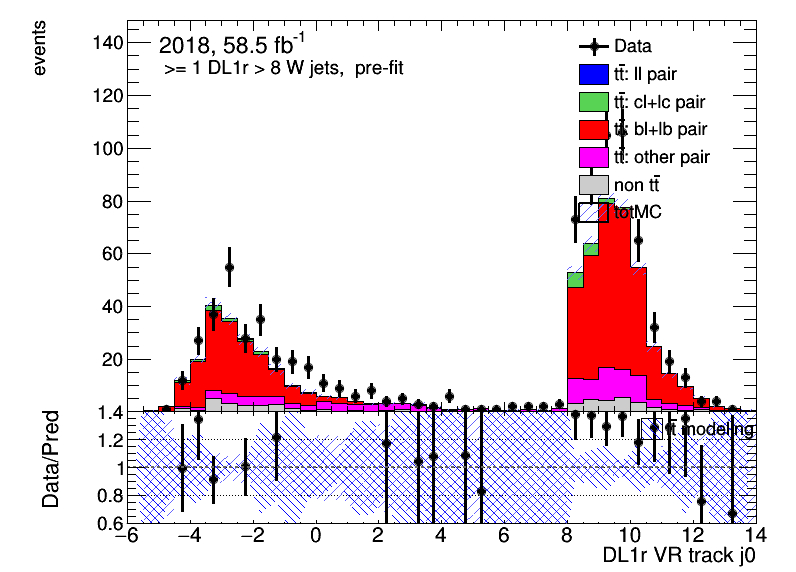
\includegraphics[width=1\textwidth]{3bplots/3bplots.png}
\end{minipage}
	\caption{The DL1r score distribution of the leading VR-Track jet, 
	requiring at least 1 VR-Track jets have DL1r > 8 to reject most of 
	the light and the $c$ jets, with $t\bar{t}$ modelling and stats uncertainties. }
    \label{fig:3bplots}
\end{figure}


\subsection{Results}
\label{result}


\subsubsection{Overview}
Four rounds of calibrations have been carried out, containing different 
jet collections, Monte Carlo samples, analysis framework 
and $b$-jet identification algorithm. In the latest round, 
the calibration includes the EMPFlow jet and VR-Track jet collection, 
and MV2c10, DL1 and DL1r taggers. Each calibration is carried out 
with all supported jet collections and taggers, with the full data 
set collected from 2015 to 2018 in the ATLAS detector. The low-$p_T$ 
selection and the standard selection are carried out for all four 
calibrations, while the high-$p_T$ selection is only implemented 
in the latest calibration. 

\subsubsection{Kinematic distributions}
The kinematic distributions of the MC and the data of the latest calibration 
(October 2020) are shwon in Figure \ref{fig:taggers_PFlow} for the PFlow jets and 
Figure \ref{fig:taggers_VRJets} for the VR-Track jets, 
combining the standard selection and the highest $p_T$ selection. 
%%%%%%%TODO: edit this%%%%%%%%
In these figure, the data events are compared against the simulation.
The majority of the events come from \ttbar\ production. There is only
a very small fraction of events, which is denoted as ``non \ttbar''
on the figure, which comes from other processes like $W$ or $Z$ production
in association with jets or single-top production. The simulated \ttbar\
events are split according to the origin of $W$-jets. The notation
``\ttbar, ll'' denotes that both $W$-jets are light flavour jets.
Similarly, ``\ttbar, cl'' (``\ttbar, bl'') 
indicates that one of the $W$-jets is a \cjet\ (\bjet)
whereas the other is a light flavour jet. $W$-jets with origin
other than what is discussed above fall into the 
category denoted by ``\ttbar, other''. This category includes
events in which at least one of the $W$-jets comes from a
hadronically decaying $\tau$-lepton. 
\begin{figure}[H]
	\begin{minipage}[b]{.45\textwidth}
	\centering
	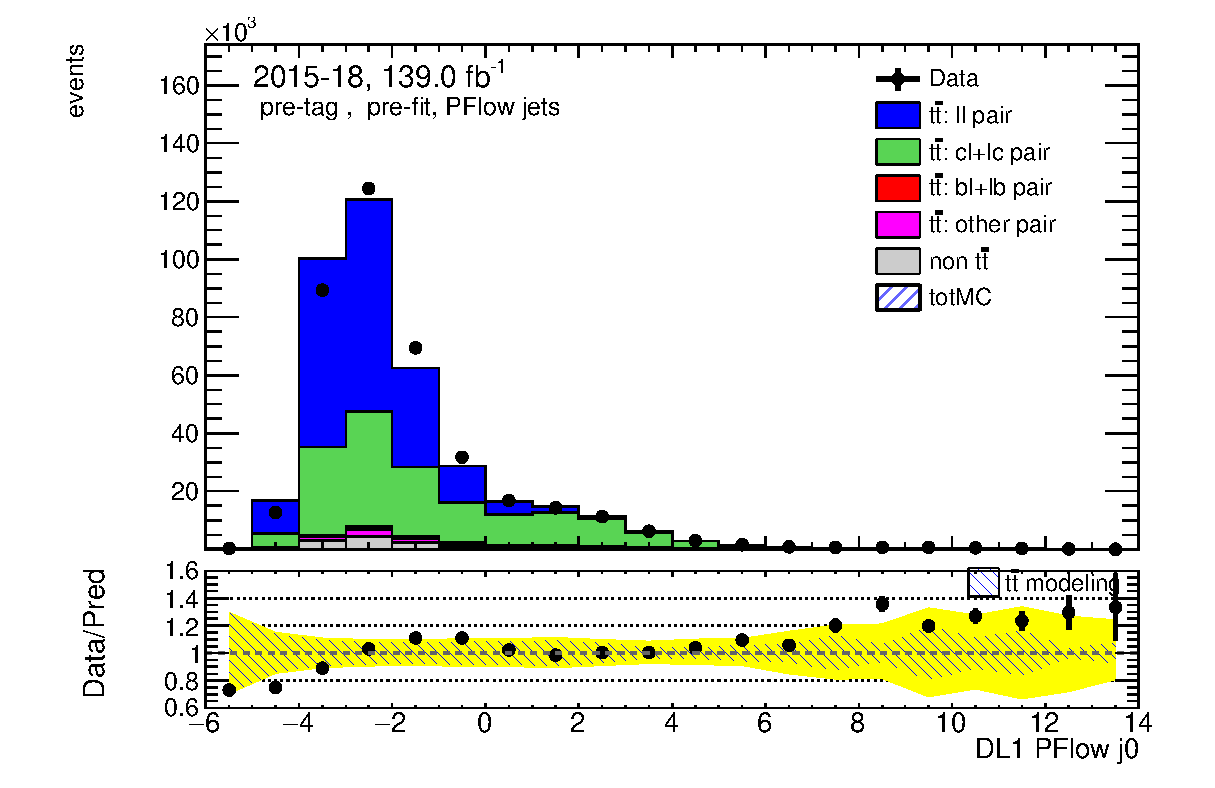
\includegraphics[width=1\textwidth]{Oct_distributions/pretagNoRwDL1rwithhighpTPFlow_scaledall/DataMC__J0_DL1.eps}
	\end{minipage}\hfill
	\begin{minipage}[b]{.45\textwidth}
	\centering
	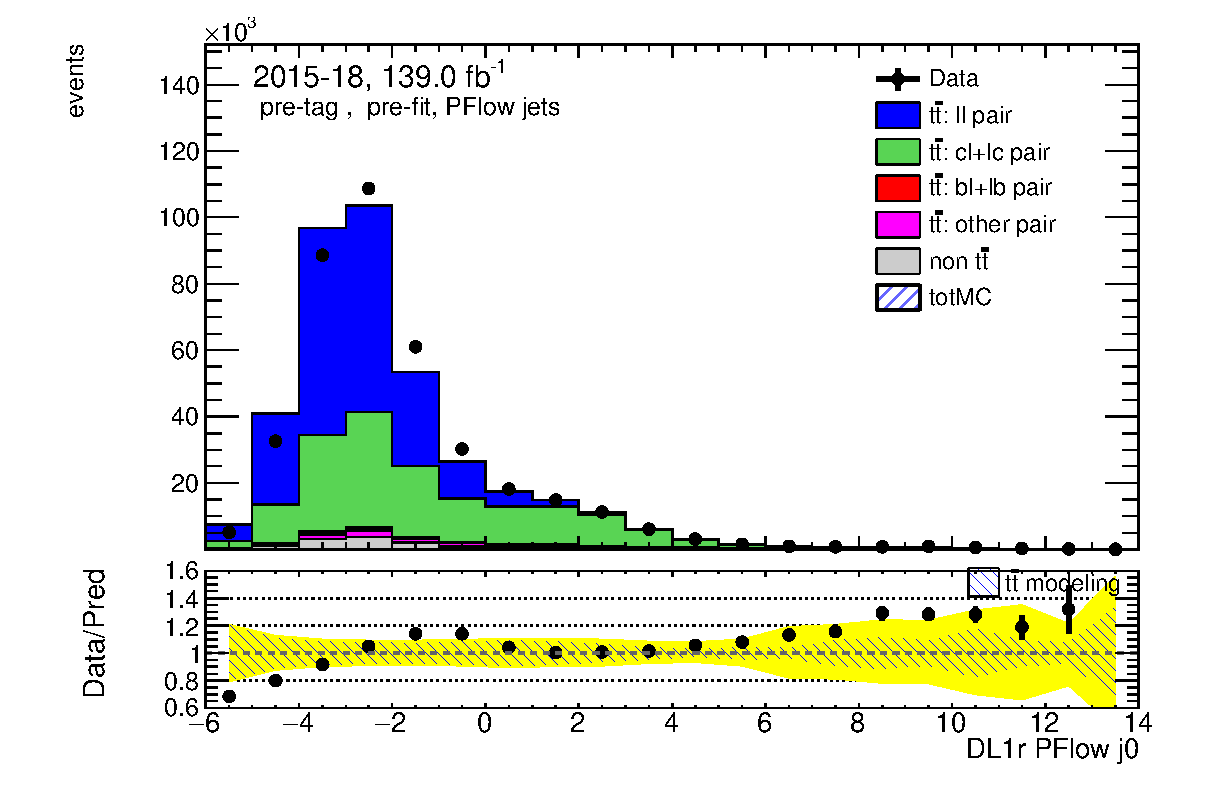
\includegraphics[width=1\textwidth]{Oct_distributions/pretagNoRwDL1rwithhighpTPFlow_scaledall/DataMC__J0_DL1r.eps}
	\end{minipage}\hfill
	\begin{minipage}[b]{.45\textwidth}
	\centering
	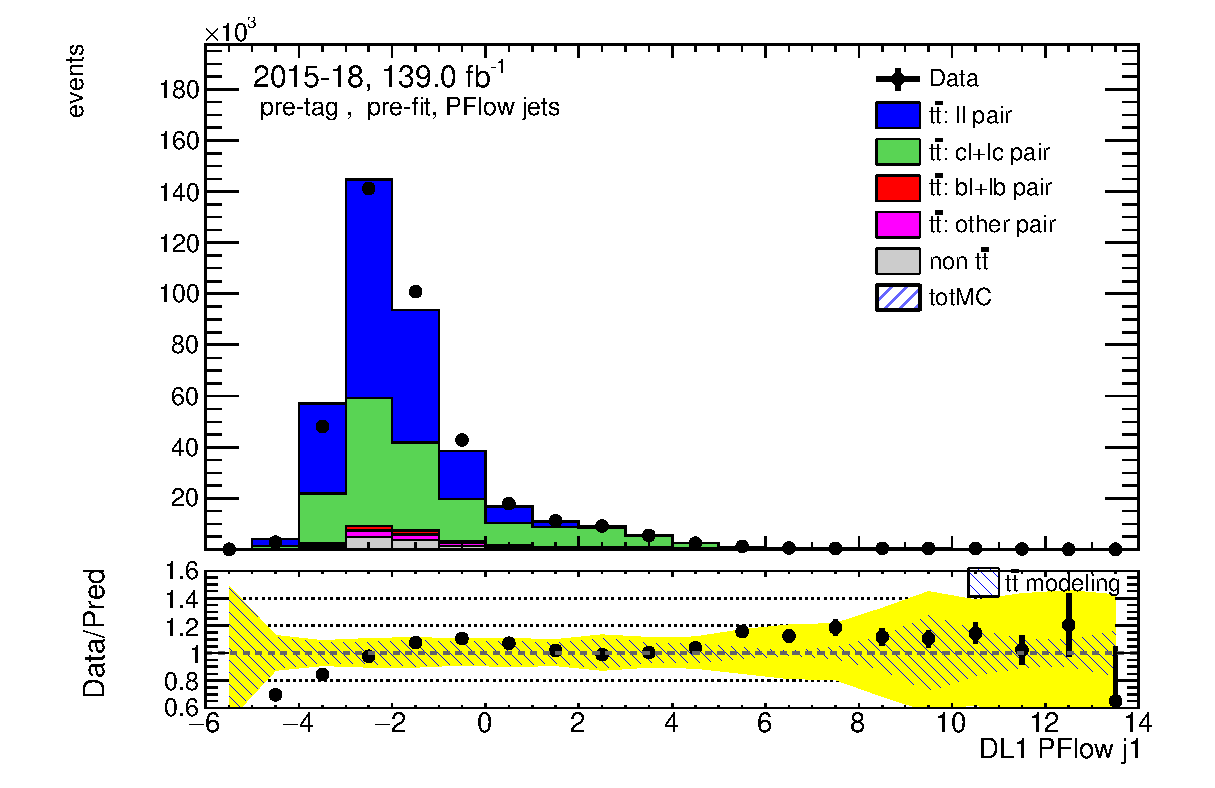
\includegraphics[width=1\textwidth]{Oct_distributions/pretagNoRwDL1rwithhighpTPFlow_scaledall/DataMC__J1_DL1.eps}
	\end{minipage}\hfill
	\begin{minipage}[b]{.45\textwidth}
	\centering
	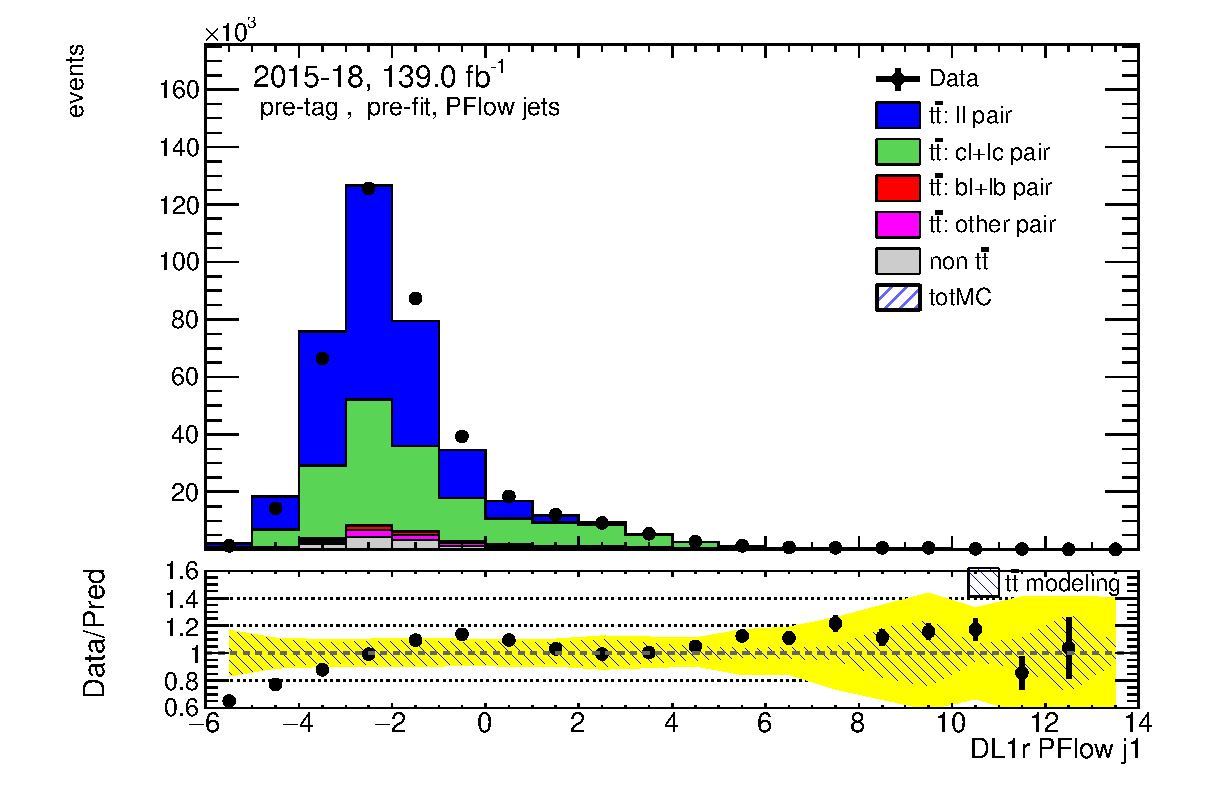
\includegraphics[width=1\textwidth]{Oct_distributions/pretagNoRwDL1rwithhighpTPFlow_scaledall/DataMC__J1_DL1r.eps}
	\end{minipage}\hfill
	\begin{minipage}[b]{.45\textwidth}
	\centering
	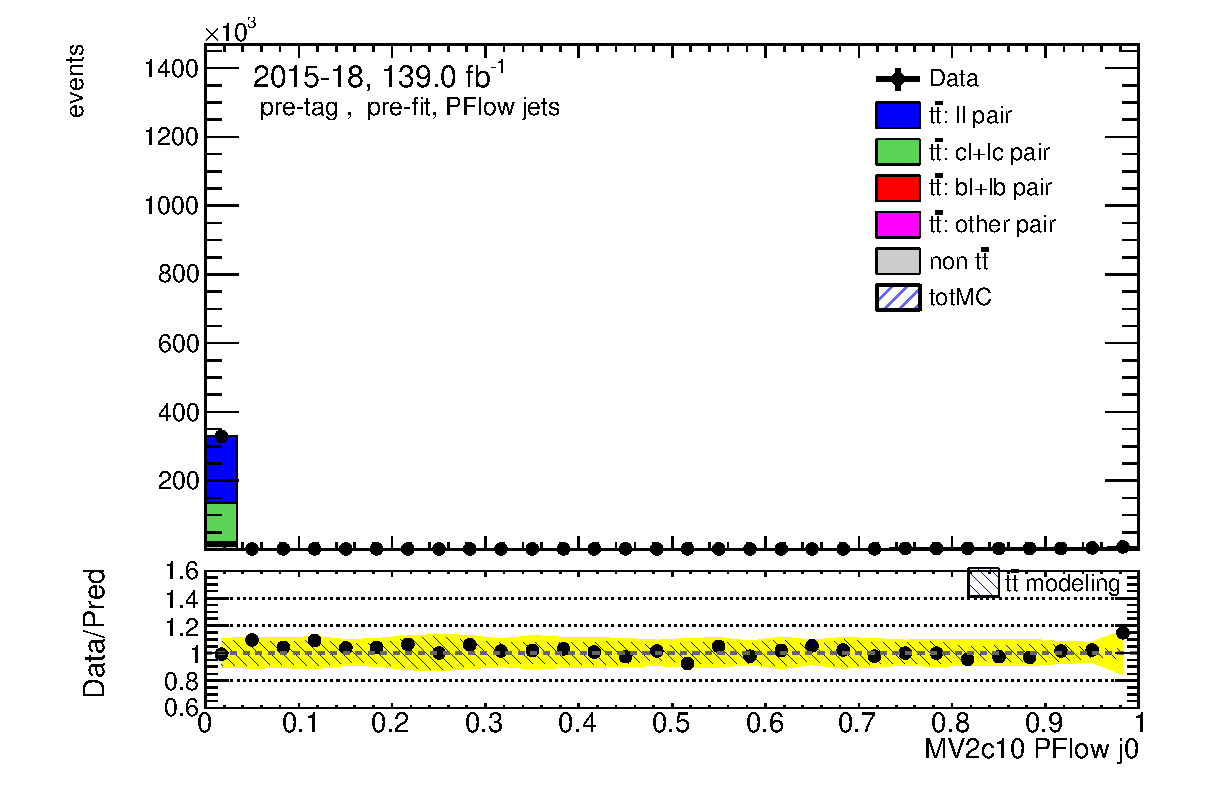
\includegraphics[width=1\textwidth]{Oct_distributions/pretagNoRwDL1rwithhighpTPFlow_scaledall/DataMC_J0_MV2c10.eps}
	\end{minipage}\hfill
	\begin{minipage}[b]{.45\textwidth}
	\centering
	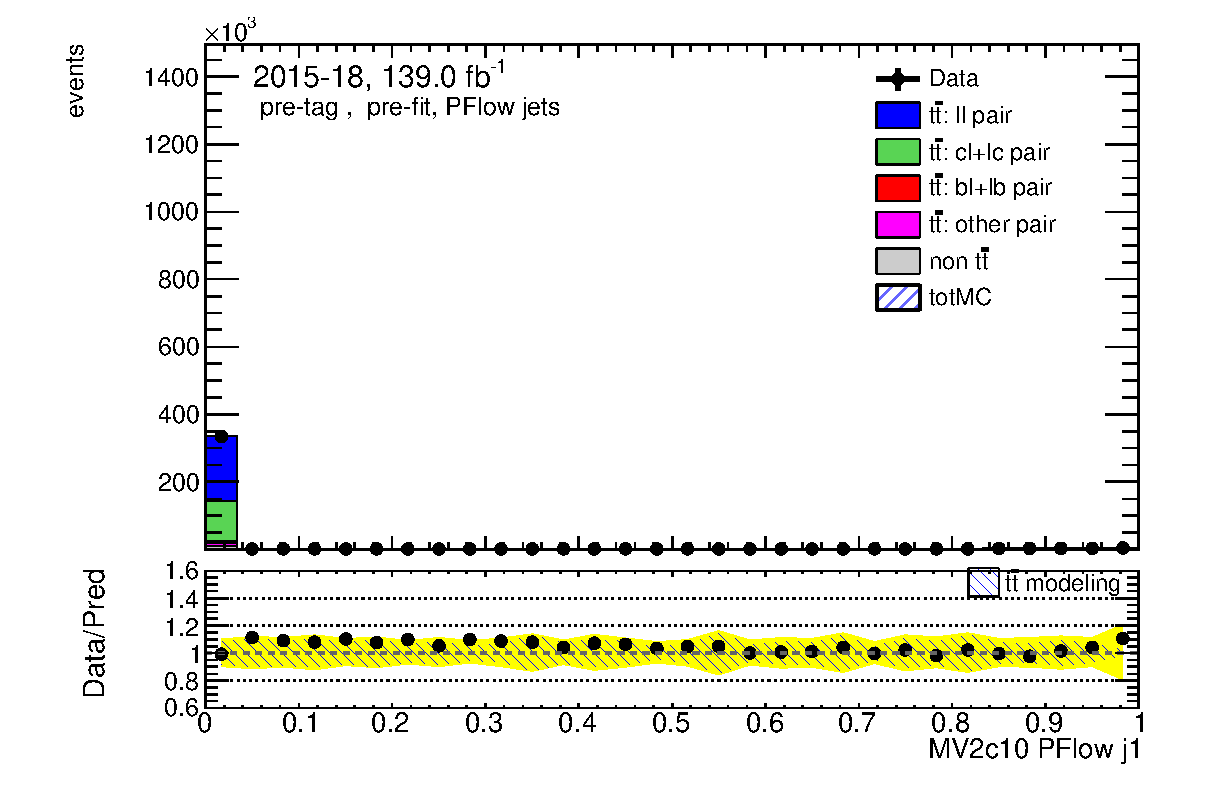
\includegraphics[width=1\textwidth]{Oct_distributions/pretagNoRwDL1rwithhighpTPFlow_scaledall/DataMC_J1_MV2c10.eps}
	\end{minipage}
	\caption{Distributions of the DL1, DL1r and MV2c10 
	taggers output of the combination 
	of the standard selection and the high-$p_T$ selection, 
	before fitting or tagging with full uncertainties.} \label{fig:taggers_PFlow}
\end{figure}

\begin{figure}[h]
	\begin{minipage}[b]{.45\textwidth}
	\centering
	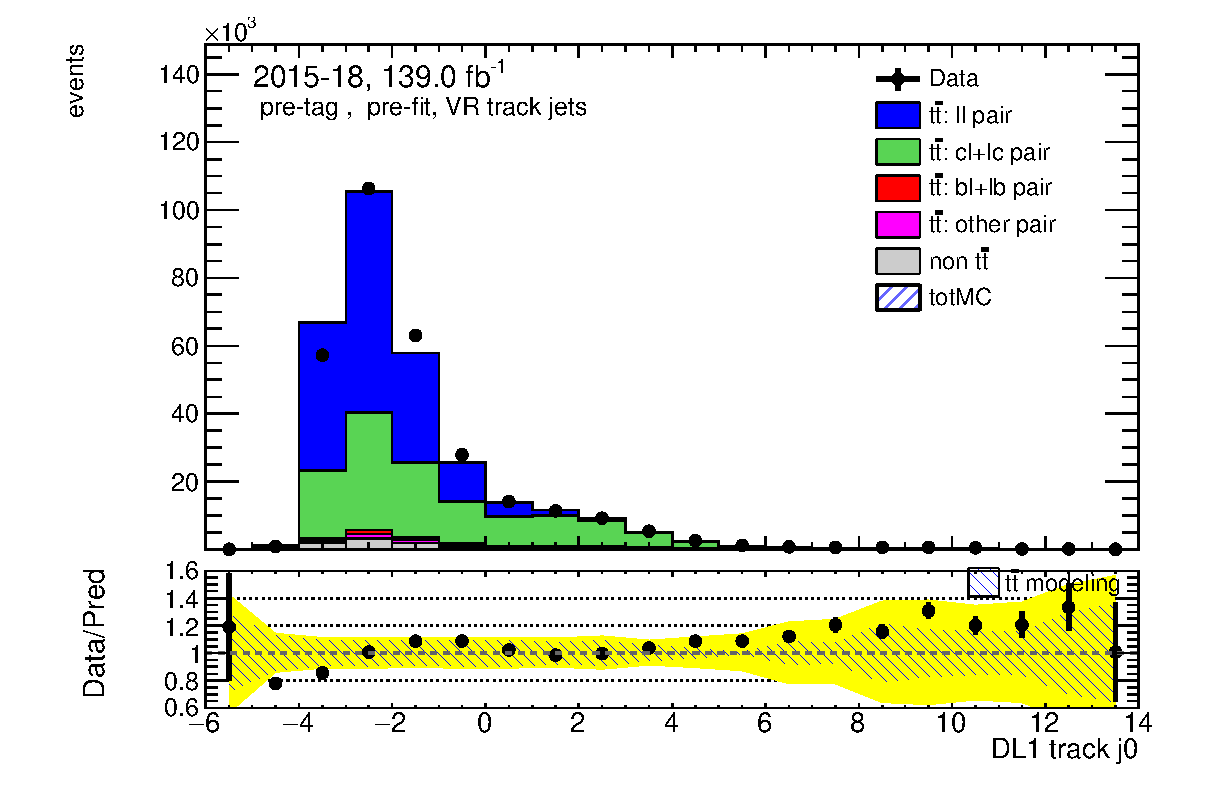
\includegraphics[width=1\textwidth]{Oct_distributions/pretagNoRwDL1rwithhighpTVRJets_scaledall/DataMC__J0_DL1.eps}
	\end{minipage}\hfill
	\begin{minipage}[b]{.45\textwidth}
	\centering
	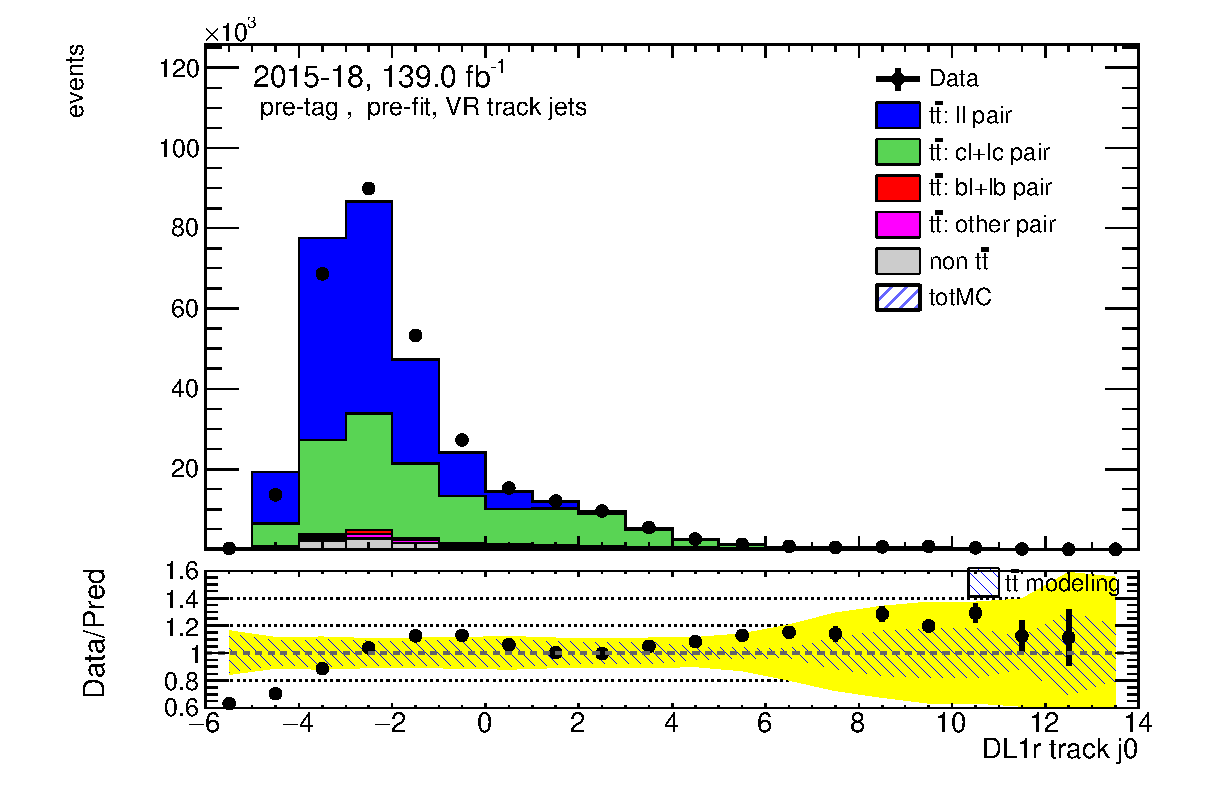
\includegraphics[width=1\textwidth]{Oct_distributions/pretagNoRwDL1rwithhighpTVRJets_scaledall/DataMC__J0_DL1r.eps}
	\end{minipage}\hfill
	\begin{minipage}[b]{.45\textwidth}
	\centering
	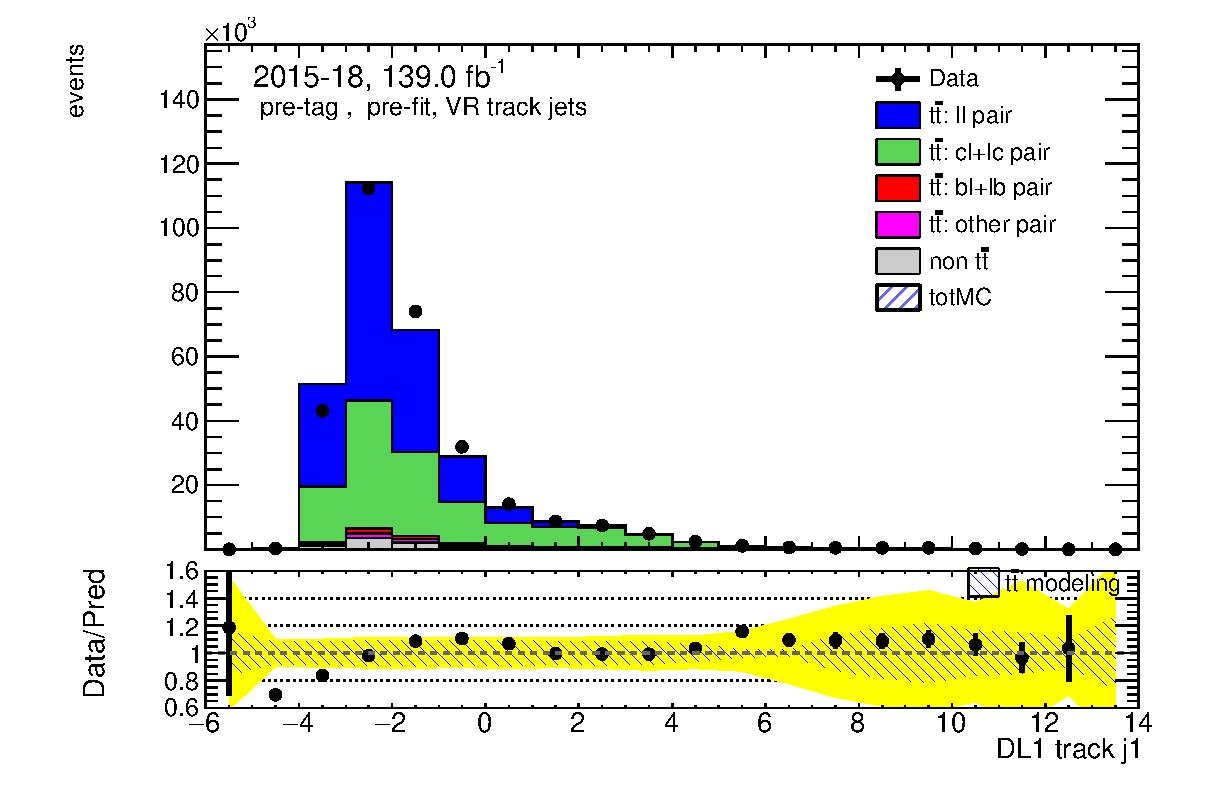
\includegraphics[width=1\textwidth]{Oct_distributions/pretagNoRwDL1rwithhighpTVRJets_scaledall/DataMC__J1_DL1.eps}
	\end{minipage}\hfill
	\begin{minipage}[b]{.45\textwidth}
	\centering
	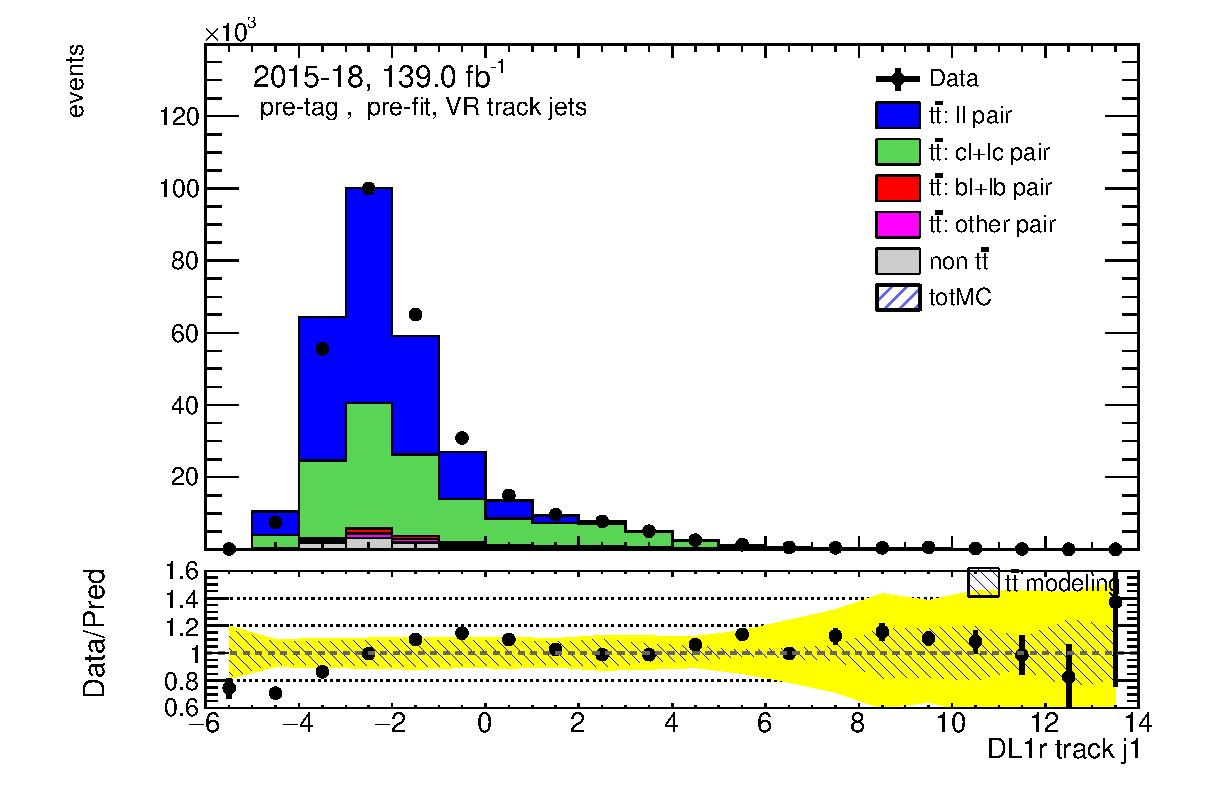
\includegraphics[width=1\textwidth]{Oct_distributions/pretagNoRwDL1rwithhighpTVRJets_scaledall/DataMC__J1_DL1r.eps}
	\end{minipage}\hfill
	\begin{minipage}[b]{.45\textwidth}
	\centering
	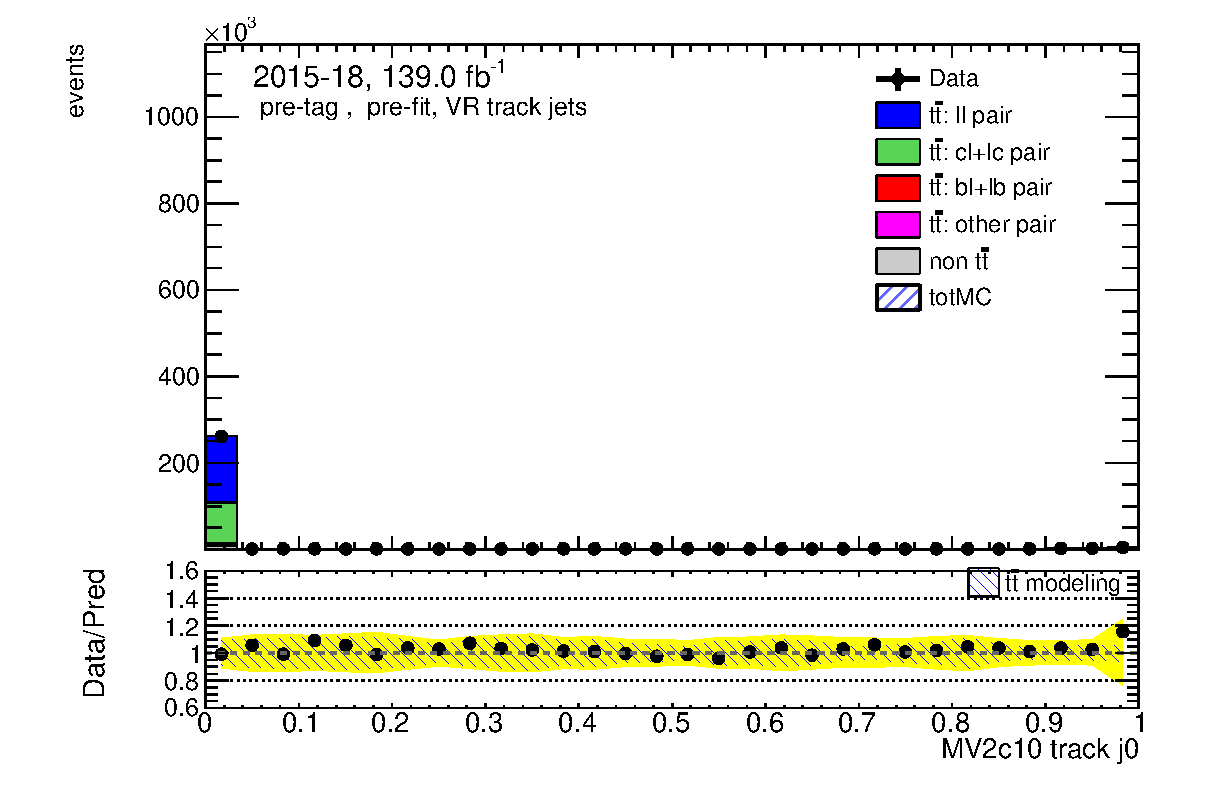
\includegraphics[width=1\textwidth]{Oct_distributions/pretagNoRwDL1rwithhighpTVRJets_scaledall/DataMC_J0_MV2c10.eps}
	\end{minipage}\hfill
	\begin{minipage}[b]{.45\textwidth}
	\centering
	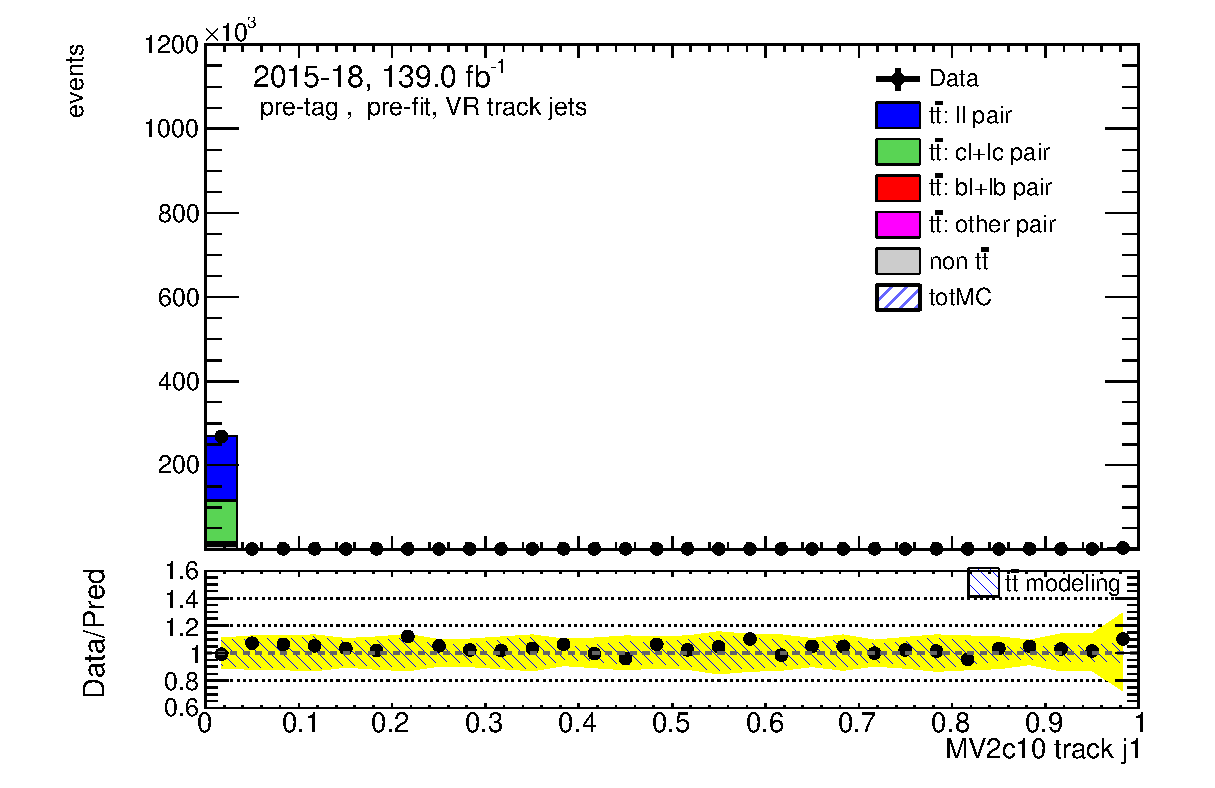
\includegraphics[width=1\textwidth]{Oct_distributions/pretagNoRwDL1rwithhighpTVRJets_scaledall/DataMC_J1_MV2c10.eps}
	\end{minipage}
	\caption{Distributions of the DL1, DL1r and MV2c10 taggers output of 
	the combination of the standard selection and the high-$p_T$ selection, 
	before fitting or tagging with full uncertainties.} \label{fig:taggers_VRJets}
	\end{figure}	

\subsubsection{Efficiencies and Scale Factors}

%The Monte Carlo simulation demonstrates good agreement in different kinematic variables with data. 
The Dl1 and DL1r $c$-jet efficiencies and scale factors with systematics 
uncertainties are calculated with 4 different fixed cut working points: 
60\%, 70\%, 77\%, and 85\%, for the p4060 derivation, in December 2020. 
The results are shown in Figure \ref{fig:Dec_eff_PFlow}, \ref{fig:Dec_eff_VRJets}, 
\ref{fig:Dec_SF_PFlow}, \ref{fig:Dec_SF_VRJets}, for the charm jets mistagging efficiency 
and scale factors for the PFlow jet collections and the VR Track jets collections. 
These results combine the standard selection and the high $p_T$ selection, 
and a 1.25 $\pm$ 0.25 scale factor is applied on events with 3 true $b$ jets. 
The $c$-jets efficiencies and the scale factors are similar between the DL1 and DL1r as expected. 


%%% Efficiencies plots %%%
\begin{figure}[H]
\begin{minipage}[b]{.45\textwidth}
\centering
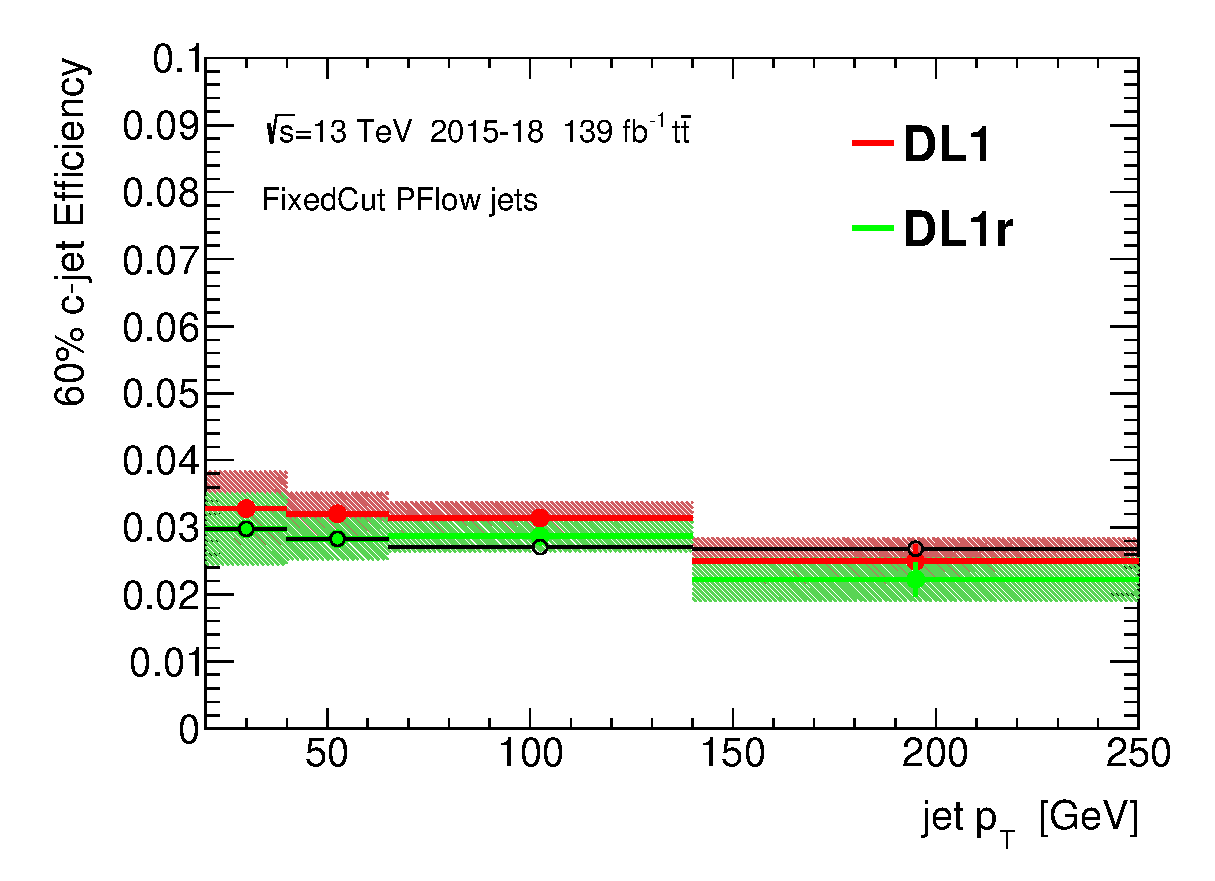
\includegraphics[width=1\textwidth]{SFplots_december/DL1allPFlowDec_DL1rallPFlowDec/eff60.eps}
\end{minipage}\hfill
\begin{minipage}[b]{.45\textwidth}
\centering
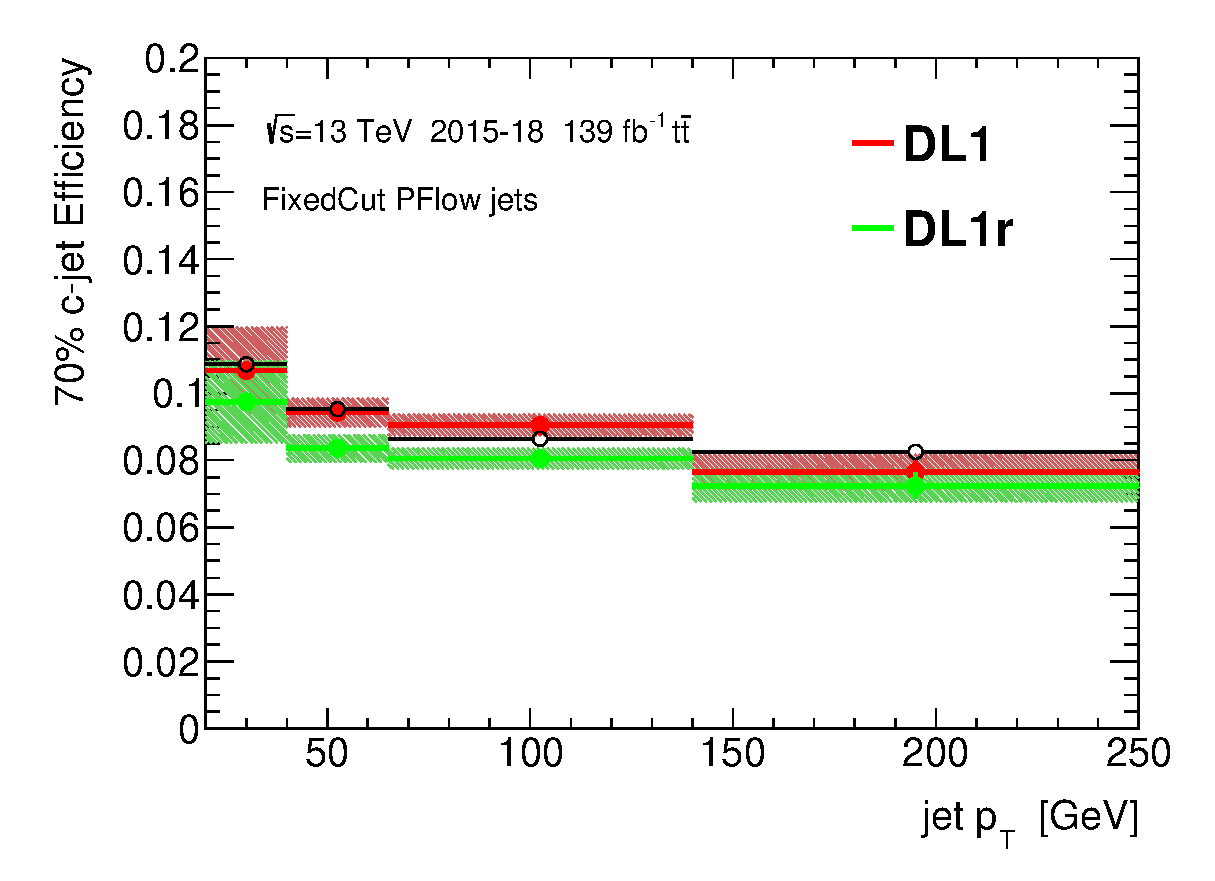
\includegraphics[width=1\textwidth]{SFplots_december/DL1allPFlowDec_DL1rallPFlowDec/eff70.eps}
\end{minipage}\hfill
\begin{minipage}[b]{.45\textwidth}
\centering
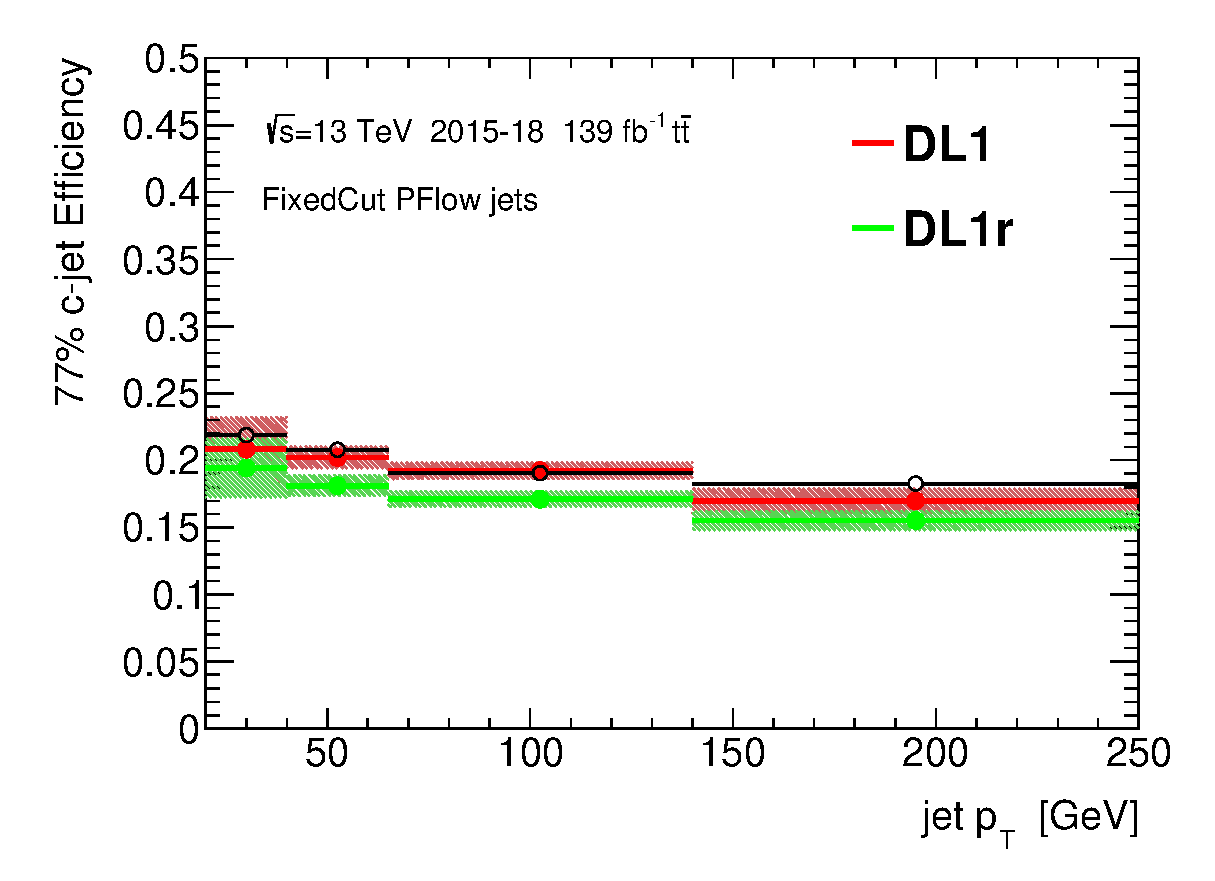
\includegraphics[width=1\textwidth]{SFplots_december/DL1allPFlowDec_DL1rallPFlowDec/eff77.eps}
\end{minipage}\hfill
\begin{minipage}[b]{.45\textwidth}
\centering
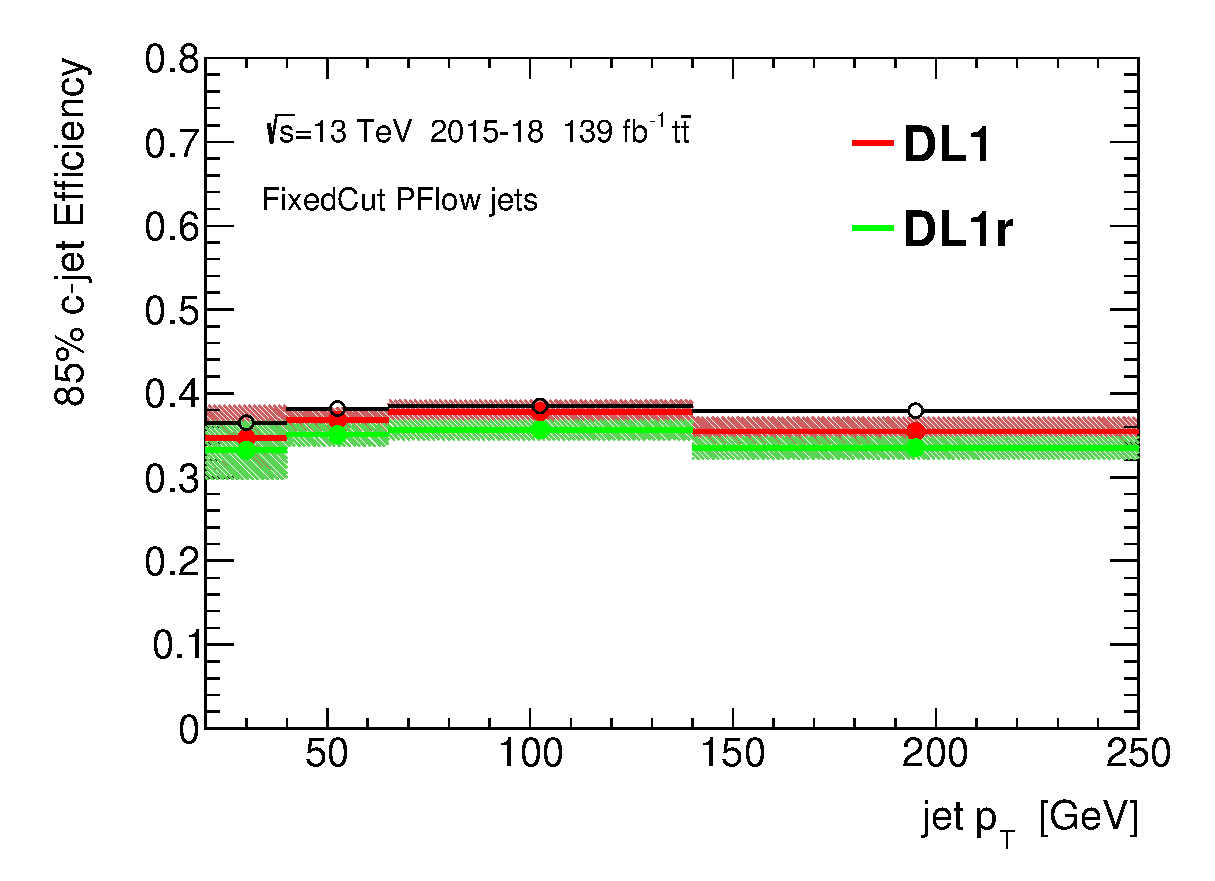
\includegraphics[width=1\textwidth]{SFplots_december/DL1allPFlowDec_DL1rallPFlowDec/eff85.eps}
\end{minipage}
\caption{Charm-jet efficiencies of PFlow jets collection of derivation 
p4060 in December 2020, given for 4 different working points.} \label{fig:Dec_eff_PFlow}
\end{figure}

\begin{figure}[H]
\begin{minipage}[b]{.45\textwidth}
\centering
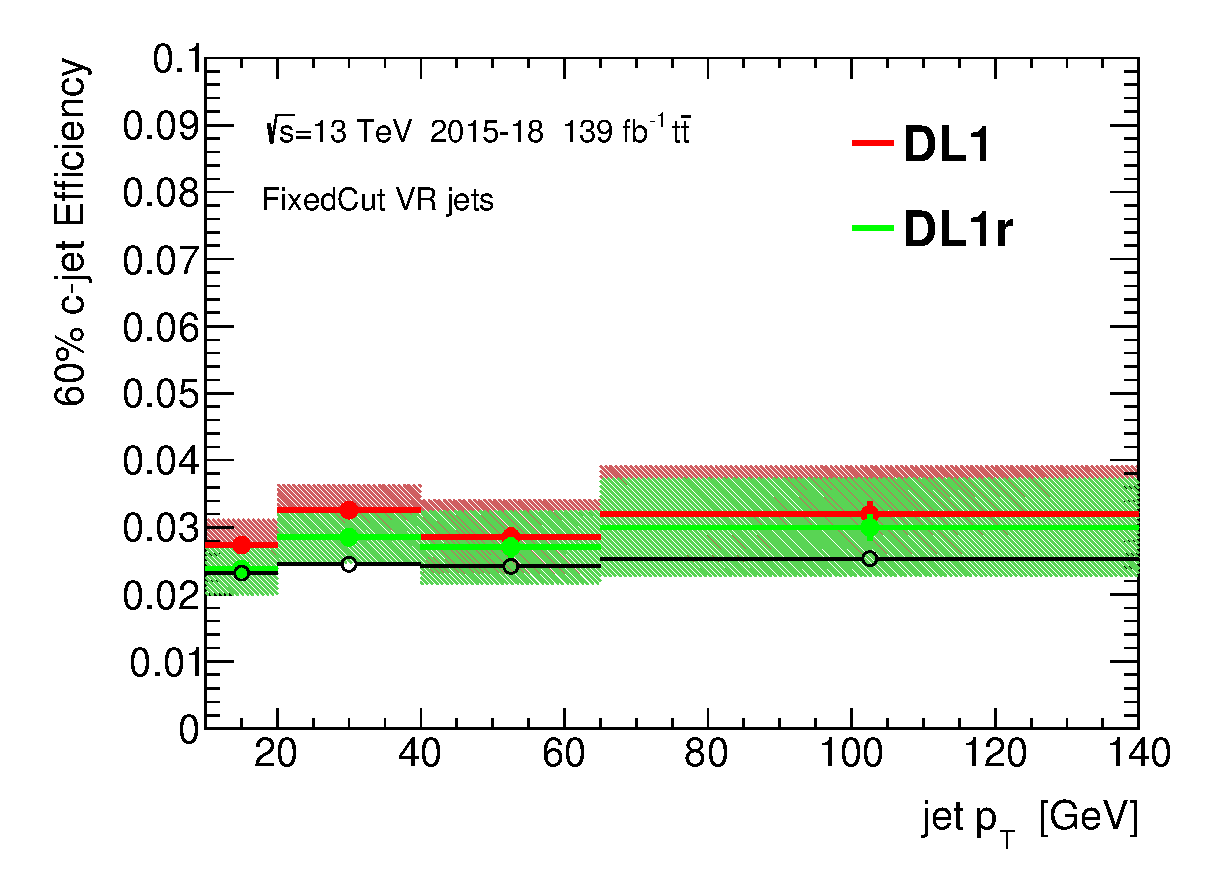
\includegraphics[width=1\textwidth]{SFplots_december/DL1allVRJetsDec_DL1rallVRJetsDec/eff60.eps}
\end{minipage}\hfill
\begin{minipage}[b]{.45\textwidth}
\centering
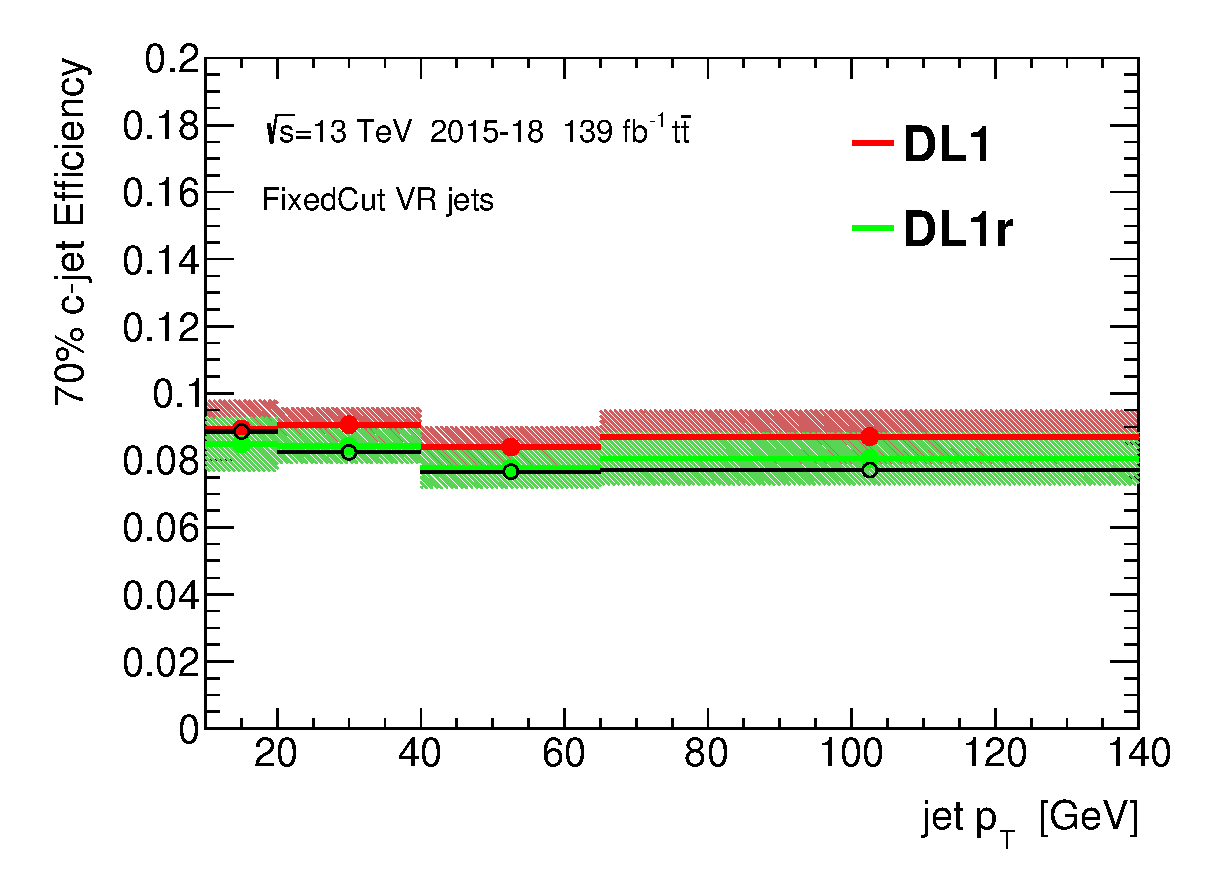
\includegraphics[width=1\textwidth]{SFplots_december/DL1allVRJetsDec_DL1rallVRJetsDec/eff70.eps}
\end{minipage}\hfill
\begin{minipage}[b]{.45\textwidth}
\centering
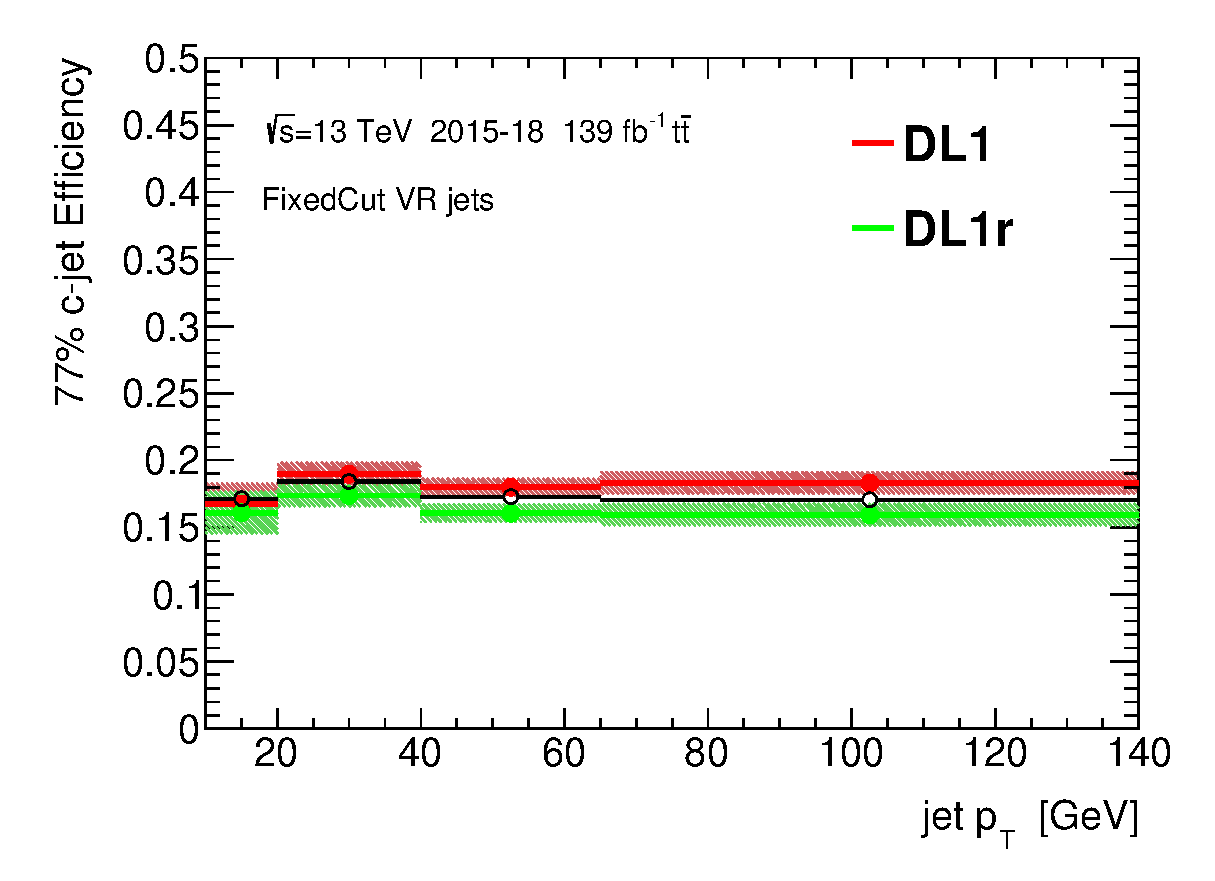
\includegraphics[width=1\textwidth]{SFplots_december/DL1allVRJetsDec_DL1rallVRJetsDec/eff77.eps}
\end{minipage}\hfill
\begin{minipage}[b]{.45\textwidth}
\centering
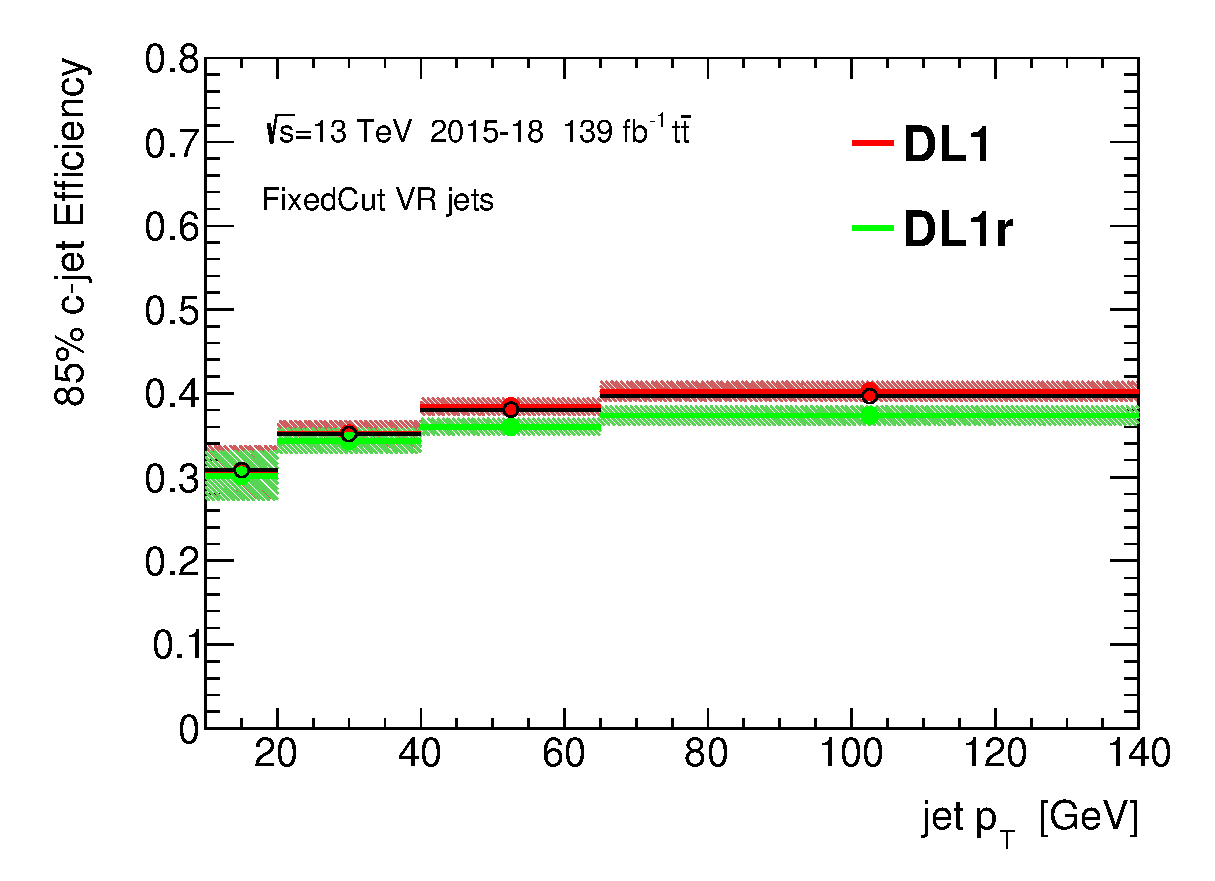
\includegraphics[width=1\textwidth]{SFplots_december/DL1allVRJetsDec_DL1rallVRJetsDec/eff85.eps}
\end{minipage}
\caption{Charm-jet efficiencies of VR-Track jets collection of derivation 
p4060 in December 2020, given for 4 different working points.} \label{fig:Dec_eff_VRJets}
\end{figure}

% SF plots

\begin{figure}[H]
\begin{minipage}[b]{.45\textwidth}
\centering
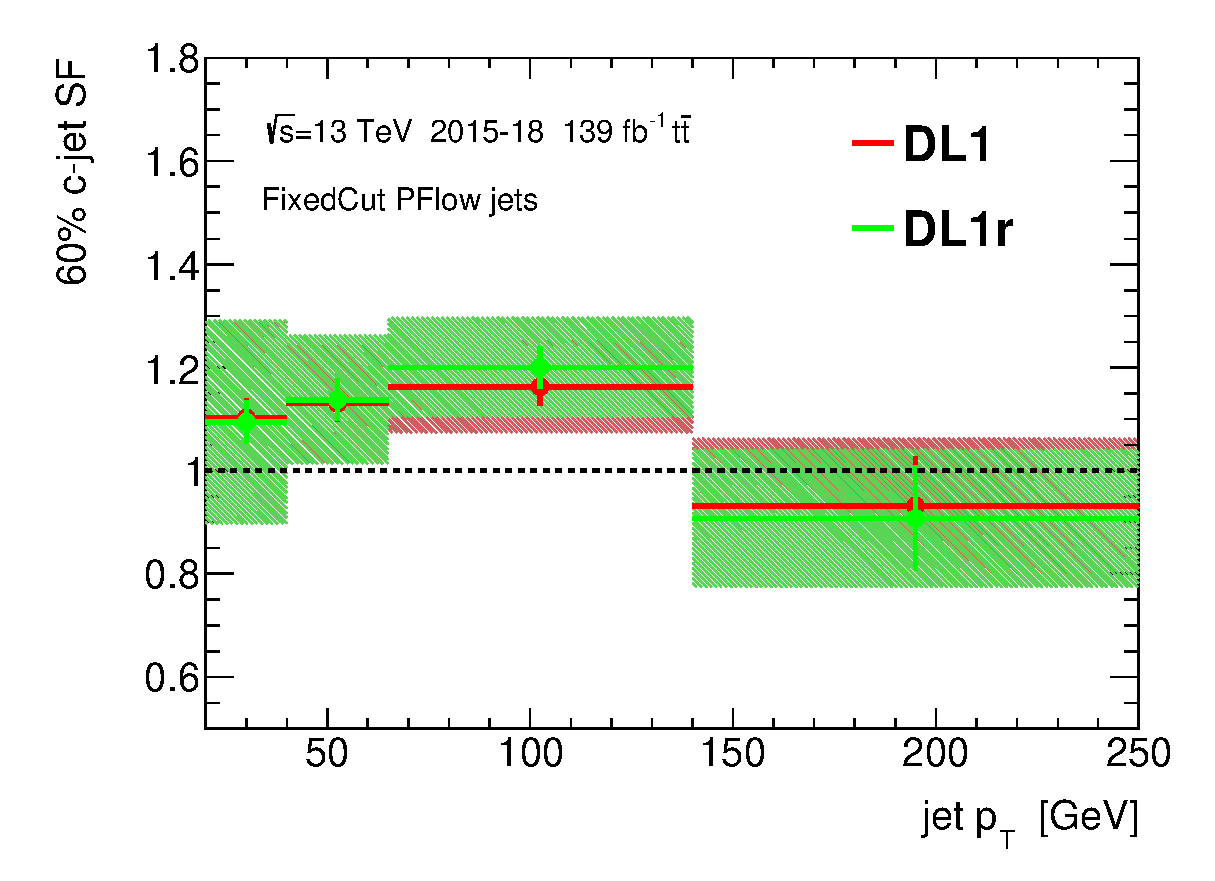
\includegraphics[width=1\textwidth]{SFplots_december/DL1allPFlowDec_DL1rallPFlowDec/SF60.eps}
\end{minipage}\hfill
\begin{minipage}[b]{.45\textwidth}
\centering
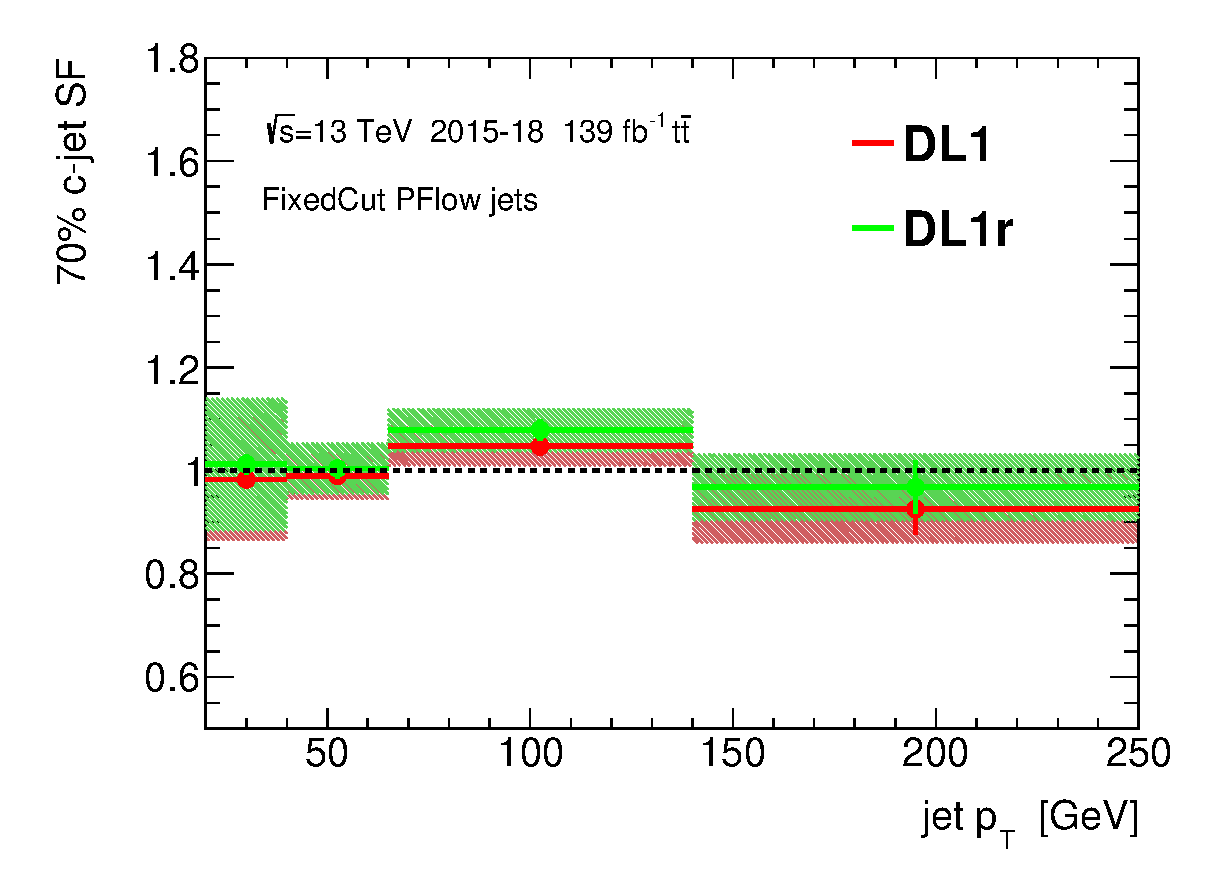
\includegraphics[width=1\textwidth]{SFplots_december/DL1allPFlowDec_DL1rallPFlowDec/SF70.eps}
\end{minipage}\hfill
\begin{minipage}[b]{.45\textwidth}
\centering
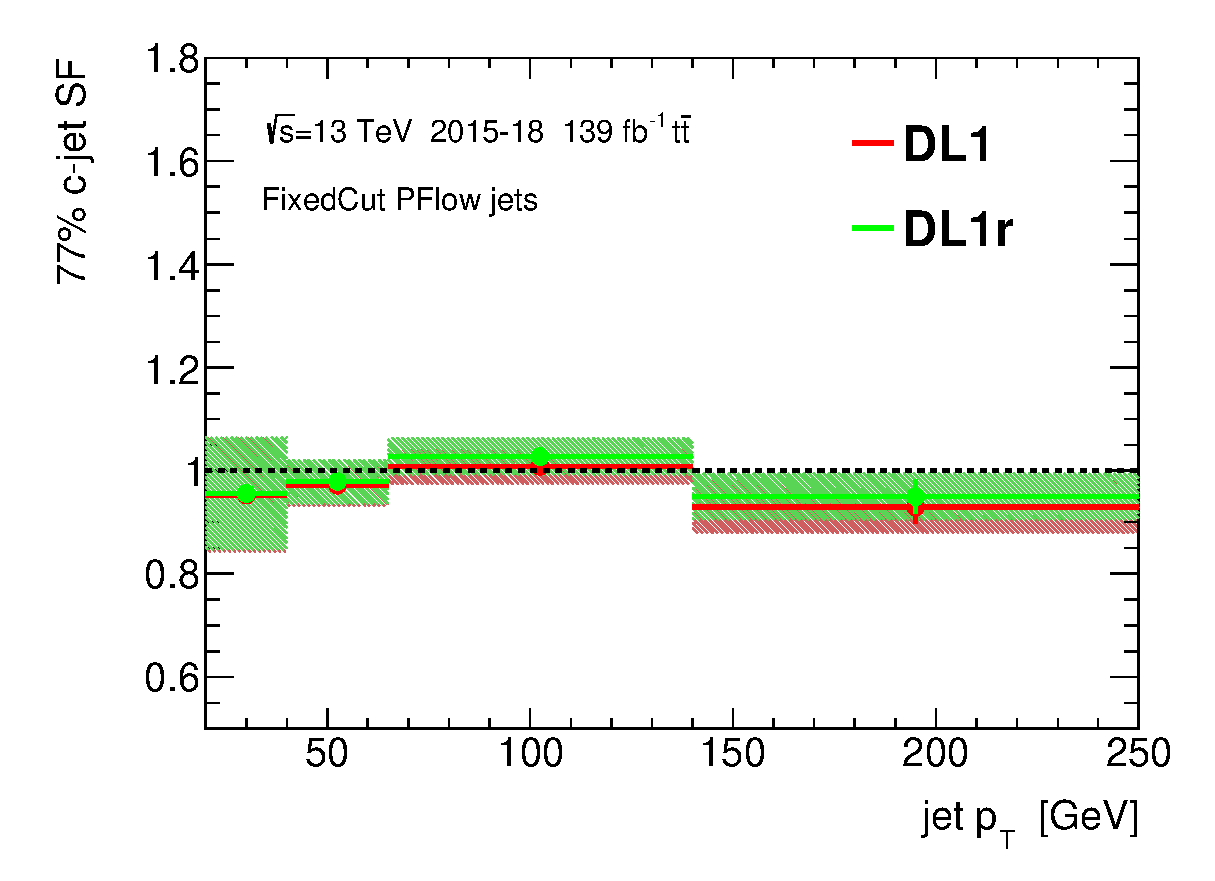
\includegraphics[width=1\textwidth]{SFplots_december/DL1allPFlowDec_DL1rallPFlowDec/SF77.eps}
\end{minipage}\hfill
\begin{minipage}[b]{.45\textwidth}
\centering
\includegraphics[width=1\textwidth]{SFplots_december/DL1allPFlowDec_DL1rallPFlowDec/SF85.eps}
\end{minipage}
\caption{Charm-jet scale factors of PFlow jets collection of derivation 
p4060 in December 2020, given for 4 different working points.} \label{fig:Dec_SF_PFlow}
\end{figure}

\begin{figure}[H]
\begin{minipage}[b]{.45\textwidth}
\centering
\includegraphics[width=1\textwidth]{SFplots_december/DL1allVRJetsDec_DL1rallVRJetsDec/SF60.eps}
\end{minipage}\hfill
\begin{minipage}[b]{.45\textwidth}
\centering
\includegraphics[width=1\textwidth]{SFplots_december/DL1allVRJetsDec_DL1rallVRJetsDec/SF70.eps}
\end{minipage}\hfill
\begin{minipage}[b]{.45\textwidth}
\centering
\includegraphics[width=1\textwidth]{SFplots_december/DL1allVRJetsDec_DL1rallVRJetsDec/SF77.eps}
\end{minipage}\hfill
\begin{minipage}[b]{.45\textwidth}
\centering
\includegraphics[width=1\textwidth]{SFplots_december/DL1allVRJetsDec_DL1rallVRJetsDec/SF85.eps}
\end{minipage}
\caption{Charm-jet scale factors of VR-Track jets collection of derivation 
p4060 in December 2020, given for 4 different working points.} \label{fig:Dec_SF_VRJets}
\end{figure}


% maybe not neccessary to include the pseudocontinuous plots 

\iffalse
\begin{figure}[H]
\begin{minipage}[b]{.45\textwidth}
\centering
\includegraphics[width=1\textwidth]{SFplots_december/DL1allPFlowDec_DL1rallPFlowDec/SF60.eps}
\end{minipage}\hfill
\begin{minipage}[b]{.45\textwidth}
\centering
\includegraphics[width=1\textwidth]{SFplots_december/DL1allPFlowDec_DL1rallPFlowDec/SF70.eps}
\end{minipage}\hfill
\begin{minipage}[b]{.45\textwidth}
\centering
\includegraphics[width=1\textwidth]{SFplots_december/DL1allPFlowDec_DL1rallPFlowDec/SF77.eps}
\end{minipage}\hfill
\begin{minipage}[b]{.45\textwidth}
\centering
\includegraphics[width=1\textwidth]{SFplots_december/DL1allPFlowDec_DL1rallPFlowDec/SF85.eps}
\end{minipage}
\caption{Scale factors of calibration of derivation p3970 in March 2020, given for  4 different working points.} \label{fig:March}
\end{figure}



\begin{figure}[H]
\begin{minipage}[b]{.45\textwidth}
\centering
\includegraphics[width=1\textwidth]{March_highpT/eff60.eps}
\end{minipage}\hfill
\begin{minipage}[b]{.45\textwidth}
\centering
\includegraphics[width=1\textwidth]{March_highpT/eff70.eps}
\end{minipage}\hfill
\begin{minipage}[b]{.45\textwidth}
\centering
\includegraphics[width=1\textwidth]{March_highpT/eff77.eps}
\end{minipage}\hfill
\begin{minipage}[b]{.45\textwidth}
\centering
\includegraphics[width=1\textwidth]{March_highpT/eff85.eps}
\end{minipage}
\caption{Charm-jet efficiencies of calibration of derivation p3970 in March 2020, combining the standard 
and the high-$p_{T}$ selection, given for  4 different working points.} \label{fig:March_highpT_eff}
\end{figure}


\begin{figure}[H]
\begin{minipage}[b]{.45\textwidth}
\centering
\includegraphics[width=1\textwidth]{March_highpT/SF60.eps}
\end{minipage}\hfill
\begin{minipage}[b]{.45\textwidth}
\centering
\includegraphics[width=1\textwidth]{March_highpT/SF70.eps}
\end{minipage}\hfill
\begin{minipage}[b]{.45\textwidth}
\centering
\includegraphics[width=1\textwidth]{March_highpT/SF77.eps}
\end{minipage}\hfill
\begin{minipage}[b]{.45\textwidth}
\centering
\includegraphics[width=1\textwidth]{March_highpT/SF85.eps}
\end{minipage}
\caption{Scale factors of calibration of derivation p3970 in March 2020, combining the standard and the high-$p_{T}$ selection, given for  4 different working points.} \label{fig:March_highpT}
\end{figure}



In terms of statistical gain, taking the 60\% working point scale factor with 2018 data as an example, the error is reduced as expected. In the last bin of the $p_{T}$ distribution of scale factors, the error is reduced by 55\%, which suggests the success of high-$p_{T}$ selection method. The percentage reduction of error of each bin is given in Tab.\ref{tab:limit}:


 \begin{table}[h]
 \begin{centering}
 \begin{tabular}{|p{2.5em}||p{2.5em}|p{2.5em}|p{5em}||p{2.5em}|p{2.5em}|p{5em}||p{5em}|}
          \hline
          & \multicolumn{3}{|c||}{high-$p_{T}$ + standard selection} & \multicolumn{3}{|c||}{standard selection only} & \\  \hline\hline
          Bins& Bin Value &Bin error&Percentage error&Bin Value &Bin error&Percentage error & Error reduction\\ \hline
          Bin 1 & 1.25 & 0.12 & 10\% &1.20 & 0.13 & 11\% & 11\% \\ \hline
          Bin 2 & 1.34 & 0.10 & 8\% & 1.24 & 0.11 & 9\% & 18\% \\ \hline
          Bin 3 & 1.22 & 0.10 & 8\% & 1.04 & 0.11 & 10\% & 28\% \\ \hline
          Bin 4 & 0.98 & 0.24 & 24\% & 0.72 & 0.27 & 37\% & 55\% \\ \hline
          
 
 \end{tabular} 
 \caption{Bins values and the corresponding errors of the scale factor at 60\% working point, with 2018 data.}
 \end{centering}
 \label{tab:limit}
 \end{table}

\fi

\newpage
\printbibliography
% \begin{thebibliography}{99}

% \bibitem{Interpreting Higgs result}, Dean Carmi, et al., \textit{Interpreting LHC Higgs Results from Natural New Physics Perspective}, \href{https://arxiv.org/abs/1202.3144}{arXiv:1202.3144}[hep-ph]. 
% \bibitem{cjet} ATLAS Collaboration, \textit{Measurement of $c$-jet tagging efficiency in $t\bar{t}$ events using a likelihood approach}, Feb 2017, \small{CDS: }\href{https://cds.cern.ch/record/2243764?ln=en}{ATL-COM-PHYS-2017-073}.\normalsize
% \bibitem{PDG}M. Tanabashiet al.(Particle Data Group), \textit{Review of Particle Physics}, Phys. Rev. D98, 030001 (2018), \href{https://link.aps.org/doi/10.1103/PhysRevD.98.030001}{doi:10.1103/PhysRevD.98.030001}.
% \bibitem{tagging} ATLAS collaboration, \textit{B Tagging in ATLAS and CMS}, Sep 2017, \small{arXiv:}\href{https://arxiv.org/abs/1709.01290}{1709.01290}\normalsize



% \bibitem{CKM1}G. Abbiendi et al., \textit{A Measurement of the rate of charm production in $W$ decays}, 1022 Phys. Lett. B490 (2000) 71, \small{arXiv: }\href{https://arxiv.org/abs/hep-ex/0009020}{hep-ex/0009020}.\normalsize
% \bibitem{CKM2}K. A. Olive 1023 et al., \textit{Review of Particle Physics}, \href{https://iopscience.iop.org/article/10.1088/1674-1137/38/9/090001}{Chin. Phys. C38 (2014) 090001}.\normalsize
% \bibitem{ttbar+HF SF}ATLAS collaboration, \textit{Measurement of the Higgs boson decaying to $b$-quarks produced in association with a top-quark pair in $pp$ collisions at $\sqrt{s}$=13 TeV with the ATLAS detector}, \href{http://cdsweb.cern.ch/record/2743685/files/ATLAS-CONF-2020-058.pdf}{ATLAS-CONF-2020-058}.
% \bibitem{ATL-PHYS-PUB-2017-0132016}Optimisation of the ATLAS b-tagging performance for the 2016 LHC Run, (2016),url: https://cds.cern.ch/record/2160731.


% \end{thebibliography}
 
\newpage

\appendix
\subsection{Appendix}
\newpage
\newpage
\section{Addition plots for the standard selection}
\begin{figure}[h]
\begin{minipage}[b]{.45\textwidth}
\centering
\includegraphics[width=1\textwidth]{Distribution_March/DataMC_J0_DL1.png}
\end{minipage}\hfill
\begin{minipage}[b]{.45\textwidth}
\centering
\includegraphics[width=1\textwidth]{Distribution_March/DataMC_J0_DL1r.png}
\end{minipage}\hfill
\begin{minipage}[b]{.45\textwidth}
\centering
\includegraphics[width=1\textwidth]{Distribution_March/DataMC_J0_eta.png}
\end{minipage}\hfill
\begin{minipage}[b]{.45\textwidth}
\centering
\includegraphics[width=1\textwidth]{Distribution_March/DataMC_J0_pt.png}
\end{minipage}\hfill
\begin{minipage}[b]{.45\textwidth}
\centering
\includegraphics[width=1\textwidth]{Distribution_March/DataMC_Mbb.png}
\end{minipage}\hfill
% \begin{minipage}[b]{.45\textwidth}
% \centering
% \includegraphics[width=1\textwidth]{Distribution_March/DataMC_MET.png}
% \end{minipage}\hfill
\begin{minipage}[b]{.45\textwidth}
\centering
\includegraphics[width=1\textwidth]{Distribution_March/DataMC_mjj.png}
\end{minipage}
% \begin{minipage}[b]{.45\textwidth}
% \centering
% \includegraphics[width=1\textwidth]{Distribution_March/DataMC_dRJJ.png}
% \end{minipage}\hfill
\caption{Standard selection: various kinematic distributions of the standard 
selection before fitting or tagging with systematics. The top two plots are 
the distributions of the DL1 and Dl1r score distributions of the leading jet.} \label{fig:standard_selection}
\end{figure}

\begin{figure}[H]
\begin{minipage}[b]{.45\textwidth}
\centering
\includegraphics[width=1\textwidth]{Distribution_March/DataMC_J1_DL1.png}
\end{minipage}\hfill
\begin{minipage}[b]{.45\textwidth}
\centering
\includegraphics[width=1\textwidth]{Distribution_March/DataMC_J1_DL1r.png}
\end{minipage}\hfill
\begin{minipage}[b]{.45\textwidth}
\centering
\includegraphics[width=1\textwidth]{Distribution_March/DataMC_J1_eta.png}
\end{minipage}\hfill
\begin{minipage}[b]{.45\textwidth}
\centering
\includegraphics[width=1\textwidth]{Distribution_March/DataMC_J1_pt.png}
\end{minipage}
\caption{Selection for low-$p_T$ extension: kinematic distributions of the 
sub-leading $W$ decay jet before fitting or tagging with systematics. 
The top two plots are distributions of the DL1 and Dl1r score of the 
sub-leading jet.} \label{fig:lowpT_selection}
\end{figure}


\begin{figure}[H]
\begin{minipage}[b]{.45\textwidth}
\centering
\includegraphics[width=1\textwidth]{Distribution_March_highpT/DataMC_J0_DL1.png}
\end{minipage}\hfill
\begin{minipage}[b]{.45\textwidth}
\centering
\includegraphics[width=1\textwidth]{Distribution_March_highpT/DataMC_J0_DL1r.png}
\end{minipage}\hfill
\begin{minipage}[b]{.45\textwidth}
\centering
\includegraphics[width=1\textwidth]{Distribution_March_highpT/DataMC_J0_eta.png}
\end{minipage}\hfill
\begin{minipage}[b]{.45\textwidth}
\centering
\includegraphics[width=1\textwidth]{Distribution_March_highpT/DataMC_J0_pt.png}
\end{minipage}\hfill
\begin{minipage}[b]{.45\textwidth}
\centering
\includegraphics[width=1\textwidth]{Distribution_March_highpT/DataMC_Mbb.png}
\end{minipage}\hfill
\begin{minipage}[b]{.45\textwidth}
\centering
\includegraphics[width=1\textwidth]{Distribution_March_highpT/DataMC_mjj.png}
\end{minipage}
\caption{Various kinematic distributions of the combination of the 
standard selection and the high-$p_T$ selection, before fitting or 
tagging with stat-only uncertainties.} \label{fig:highpT_selection}
\end{figure}



\begin{figure}
\includegraphics[width=1\textwidth]{Dec_eff.png}
\caption{Calibration of derivation p3970 in December 2019, given for  4 different working points.}\label{fig:Dec_eff}
\end{figure}

\begin{figure}
\includegraphics[width=1\textwidth]{Dec.png}
\caption{Calibration result of derivation p3970 in December 2019, given for  4 different working points.}\label{fig:Dec}
\end{figure}





	
	\begin{figure}
	\begin{minipage}[b]{.45\textwidth}
	\centering
	\includegraphics[width=1\textwidth]{Oct_distributions/pretagNoRwDL1rwithhighpTPFlow_scaledall/DataMC_J0_eta.eps}
	\end{minipage}\hfill
	\begin{minipage}[b]{.45\textwidth}
	\centering
	\includegraphics[width=1\textwidth]{Oct_distributions/pretagNoRwDL1rwithhighpTPFlow_scaledall/DataMC_J1_eta.eps}
	\end{minipage}\hfill
	\begin{minipage}[b]{.45\textwidth}
	\centering
	\includegraphics[width=1\textwidth]{Oct_distributions/pretagNoRwDL1rwithhighpTPFlow_scaledall/DataMC_LLR.eps}
	\end{minipage}\hfill
	\begin{minipage}[b]{.45\textwidth}
	\centering
	\includegraphics[width=1\textwidth]{Oct_distributions/pretagNoRwDL1rwithhighpTPFlow_scaledall/DataMC_MET.eps}
	\end{minipage}
	\caption{Distributions of the leading and sub-leading jets from W decay, KLFitter output and the 
	transverse missing transverse energy of the combination of the standard selection and the 
	high-$p_T$ selection, before fitting or tagging with full uncertainties.} \label{fig:jets_PFlow}
	\end{figure}
	
	
	
	
	\begin{figure}
	\begin{minipage}[b]{.45\textwidth}
	\centering
	\includegraphics[width=1\textwidth]{Oct_distributions/pretagNoRwDL1rwithhighpTPFlow_scaledall/DataMC_dRbb.eps}
	\end{minipage}\hfill
	\begin{minipage}[b]{.45\textwidth}
	\centering
	\includegraphics[width=1\textwidth]{Oct_distributions/pretagNoRwDL1rwithhighpTPFlow_scaledall/DataMC_dRqq.eps}
	\end{minipage}\hfill
	\begin{minipage}[b]{.45\textwidth}
	\centering
	\includegraphics[width=1\textwidth]{Oct_distributions/pretagNoRwDL1rwithhighpTPFlow_scaledall/DataMC_dRbhadq1.eps}
	\end{minipage}\hfill
	\begin{minipage}[b]{.45\textwidth}
	\centering
	\includegraphics[width=1\textwidth]{Oct_distributions/pretagNoRwDL1rwithhighpTPFlow_scaledall/DataMC_dRblepq1.eps} 
	\end{minipage}\hfill
	\begin{minipage}[b]{.45\textwidth}
	\centering
	\includegraphics[width=1\textwidth]{Oct_distributions/pretagNoRwDL1rwithhighpTPFlow_scaledall/DataMC_dRWhadbhad.eps} 
	\end{minipage}\hfill
	\begin{minipage}[b]{.45\textwidth}
	\centering
	\includegraphics[width=1\textwidth]{Oct_distributions/pretagNoRwDL1rwithhighpTPFlow_scaledall/DataMC_dRWhadblep.eps} 
	\end{minipage}
	\caption{Distributions of angle related variables of the combination of the standard 
	selection and the high-$p_T$ selection, before fitting or 
	tagging with full uncertainties.} \label{fig:angles_PFlow}
	\end{figure}
	
	
	\begin{figure}
	\begin{minipage}[b]{.45\textwidth}
	\centering
	\includegraphics[width=1\textwidth]{Oct_distributions/pretagNoRwDL1rwithhighpTPFlow_scaledall/DataMC_Mbb.eps}
	\end{minipage}\hfill
	\begin{minipage}[b]{.45\textwidth}
	\centering
	\includegraphics[width=1\textwidth]{Oct_distributions/pretagNoRwDL1rwithhighpTPFlow_scaledall/DataMC_mjj.eps}
	\end{minipage}
	\begin{minipage}[b]{.45\textwidth}
	\centering
	\includegraphics[width=1\textwidth]{Oct_distributions/pretagNoRwDL1rwithhighpTPFlow_scaledall/DataMC_mjjj.eps}
	\end{minipage}\hfill
	\begin{minipage}[b]{.45\textwidth}
	\centering
	\includegraphics[width=1\textwidth]{Oct_distributions/pretagNoRwDL1rwithhighpTPFlow_scaledall/DataMC_Htjj.eps}
	\end{minipage}
	\caption{Distributions of mass related variables of the combination 
	of the standard selection and the 
	high-$p_T$ selection, before fitting or 
	tagging with stat-only uncertainties.} \label{fig:mass_PFlow}
	\end{figure}
	
	
	
	
	\begin{figure}
	\begin{minipage}[b]{.45\textwidth}
	\centering
	\includegraphics[width=1\textwidth]{Oct_distributions/pretagNoRwDL1rwithhighpTVRJets_scaledall/DataMC_J0_eta.eps}
	\end{minipage}\hfill
	\begin{minipage}[b]{.45\textwidth}
	\centering
	\includegraphics[width=1\textwidth]{Oct_distributions/pretagNoRwDL1rwithhighpTVRJets_scaledall/DataMC_J1_eta.eps}
	\end{minipage}\hfill
	\begin{minipage}[b]{.45\textwidth}
	\centering
	\includegraphics[width=1\textwidth]{Oct_distributions/pretagNoRwDL1rwithhighpTVRJets_scaledall/DataMC_LLR.eps}
	\end{minipage}\hfill
	\begin{minipage}[b]{.45\textwidth}
	\centering
	\includegraphics[width=1\textwidth]{Oct_distributions/pretagNoRwDL1rwithhighpTVRJets_scaledall/DataMC_MET.eps}
	\end{minipage}
	
	\caption{Distributions of the leading and sub-leading jets 
	from W decay, KLFitter output and the transverse missing transverse 
	energy of the combination of the standard selection and the 
	high-$p_T$ selection, before fitting or tagging with 
	full uncertainties.} \label{fig:jets_VRJets}
	\end{figure}
	
	
	
	
	\begin{figure}
	\begin{minipage}[b]{.45\textwidth}
	\centering
	\includegraphics[width=1\textwidth]{Oct_distributions/pretagNoRwDL1rwithhighpTVRJets_scaledall/DataMC_dRbb.eps}
	\end{minipage}\hfill
	\begin{minipage}[b]{.45\textwidth}
	\centering
	\includegraphics[width=1\textwidth]{Oct_distributions/pretagNoRwDL1rwithhighpTVRJets_scaledall/DataMC_dRqq.eps}
	\end{minipage}\hfill
	\begin{minipage}[b]{.45\textwidth}
	\centering
	\includegraphics[width=1\textwidth]{Oct_distributions/pretagNoRwDL1rwithhighpTVRJets_scaledall/DataMC_dRbhadq1.eps}
	\end{minipage}\hfill
	\begin{minipage}[b]{.45\textwidth}
	\centering
	\includegraphics[width=1\textwidth]{Oct_distributions/pretagNoRwDL1rwithhighpTVRJets_scaledall/DataMC_dRblepq1.eps} 
	\end{minipage}\hfill
	\begin{minipage}[b]{.45\textwidth}
	\centering
	\includegraphics[width=1\textwidth]{Oct_distributions/pretagNoRwDL1rwithhighpTVRJets_scaledall/DataMC_dRWhadbhad.eps} 
	\end{minipage}\hfill
	\begin{minipage}[b]{.45\textwidth}
	\centering
	\includegraphics[width=1\textwidth]{Oct_distributions/pretagNoRwDL1rwithhighpTVRJets_scaledall/DataMC_dRWhadblep.eps} 
	\end{minipage}
	\caption{Distributions of angle related variables of the combination 
	of the standard selection and the high-$p_T$ 
	selection, before fitting or tagging with full uncertainties.} \label{fig:angles_VRJets}
	\end{figure}
	
	
	\begin{figure}
	\begin{minipage}[b]{.45\textwidth}
	\centering
	\includegraphics[width=1\textwidth]{Oct_distributions/pretagNoRwDL1rwithhighpTVRJets_scaledall/DataMC_Mbb.eps}
	\end{minipage}\hfill
	\begin{minipage}[b]{.45\textwidth}
	\centering
	\includegraphics[width=1\textwidth]{Oct_distributions/pretagNoRwDL1rwithhighpTVRJets_scaledall/DataMC_mjj.eps}
	\end{minipage}
	\begin{minipage}[b]{.45\textwidth}
	\centering
	\includegraphics[width=1\textwidth]{Oct_distributions/pretagNoRwDL1rwithhighpTVRJets_scaledall/DataMC_mjjj.eps}
	\end{minipage}\hfill
	\begin{minipage}[b]{.45\textwidth}
	\centering
	\includegraphics[width=1\textwidth]{Oct_distributions/pretagNoRwDL1rwithhighpTVRJets_scaledall/DataMC_Htjj.eps}
	\end{minipage}
	\caption{Distributions of mass related variables of the combination 
	of the standard selection and the high-$p_T$ selection, 
	before fitting or tagging with stat-only uncertainties.} \label{fig:mass_VRJets}
	\end{figure}
	









\begin{table}[h]
\begin{centering}
\begin{tabular}{p{25em}}

          \hline
          \textbf{Systematic uncertainty}
          \\
          \hline
          \hline
        EG\_RESOLUTION\_ALL
        \\
		\hline
		MUON\_ID
		\\
		MUON\_MS
		\\
		\hline
		MET\_SoftTrk\_ResoPara
		\\
		MET\_SoftTrk\_ResoPerp
		\\
		MET\_SoftTrk\_ScaleDown
		\\
		MET\_SoftTrk\_ScaleUp
		\\
		\hline
		JET\_Pileup\_OffsetNPV
		\\
		JET\_Pileup\_RhoTopology
		\\
		\hline
		JET\_EffectiveNP\_Modelling1
		\\ 
		JET\_EffectiveNP\_Modelling2
		\\ 
		JET\_EffectiveNP\_Modelling3
		\\ 
		JET\_EffectiveNP\_Modelling4
		\\ 
		JET\_EffectiveNP\_Statistical4
		\\ 
		JET\_EffectiveNP\_Detector1
		\\ 
		\hline 
		JET\_JER\_EffectiveNP\_1
		\\ 
		JET\_JER\_EffectiveNP\_2
		\\ 
		JET\_JER\_EffectiveNP\_3
		\\ 
		JET\_JER\_EffectiveNP\_4
		\\ 
		\hline 
		JET\_BJES\_Response
		\\ 
		\hline 
		JET\_Flavor\_Composition
		\\ 
		JET\_Flavor\_Response
        \\ 
        \hline

 \end{tabular} 
 
 \end{centering}
 \caption{List of experimental systematics.}\label{tab:systematics}
 \end{table}




\end{document}
